\documentclass[11pt, oneside]{article}   	% use "amsart" instead of "article" for AMSLaTeX format
\usepackage{geometry}                		% See geometry.pdf to learn the layout options. There are lots.
\geometry{letterpaper}                   	% ... or a4paper or a5paper or ... 
%\geometry{landscape}                		% Activate for rotated page geometry
\usepackage[parfill]{parskip}    	% Activate to begin paragraphs with an empty line rather than an indent
\usepackage{graphicx}				% Use pdf, png, jpg, or eps§ with pdflatex; use eps in DVI mode
								% TeX will automatically convert eps --> pdf in pdflatex		
\usepackage{amssymb}
\usepackage{amsmath}
\usepackage{cite}
\usepackage{hyperref}
\usepackage{float}

%SetFonts


\title{Harnessing Transformers for Fraud Detection: Tackling Imbalanced Data and Outperforming Baselines}
\author{Fengyuan Shen, Jinhu Sun}
\date{December 6, 2024}		% Activate to display a given date or no date

\begin{document}
\maketitle
\begin{abstract}
This project investigates the application of a Transformer-based model for financial fraud detection, focusing on strategies to address severe class imbalance and capture complex transaction patterns. We employ SMOTE to rebalance the training data and experiment with Focal Loss to emphasize hard-to-classify cases. Our results demonstrate that the Transformer, when appropriately tuned, can surpass traditional baselines such as Logistic Regression, Random Forest, Long Short-Term Memory Network (LSTM), and Multi-Layer Perceptron (MLP) in detecting fraudulent transactions. By leveraging attention mechanisms and carefully selecting model parameters, we achieve improvements in minority-class recall without excessively compromising performance on the majority class. This work highlights the potential of advanced deep learning architectures for fraud detection and provides insights into how targeted adjustments to model training can yield substantial performance gains.
\end{abstract}


\section{Introduction}

Financial fraud poses significant risks to individuals, businesses, and the global economy, making effective detection methods essential. However, identifying fraud in credit card transactions remains challenging due to two key factors: (1) the extreme imbalance in class distribution, with fraudulent transactions constituting a tiny fraction of all activity, and (2) the complexity of transaction patterns that may not be linearly separable.

Traditional machine learning models, such as Logistic Regression and Random Forest, offer interpretability and ease of training but often struggle to capture the nuanced relationships between features in highly imbalanced datasets. Deep learning models, including LSTMs, can process sequential data and potentially uncover temporal dependencies, but their computational overhead and reliance on strictly ordered sequences may limit their scalability.

In this work, we propose employing a Transformer-based model to exploit self-attention mechanisms, enabling the capture of both local and global patterns without strict sequential processing. We address class imbalance by applying SMOTE to the training set, thus allowing our model to better focus on minority-class examples. Additionally, we incorporate Focal Loss to further highlight hard-to-classify fraud instances, ultimately improving the model’s recall on the minority class.

Our empirical results show that, while baseline models can perform surprisingly well once the data is balanced, the Transformer model, when paired with appropriate training strategies, can surpass these baselines. By carefully tuning hyperparameters—especially the Focal Loss parameter \(\gamma\)—the Transformer achieves a more favorable balance between fraud detection and false alarms. This investigation contributes to the growing body of literature on advanced deep learning methods for fraud detection, offering practical insights into managing data imbalance and tailoring loss functions to better serve real-world security needs.


\section{Related Work}

Financial fraud detection has traditionally relied on models such as Logistic Regression and Random Forest due to their simplicity and interpretability \cite{ali2022financial}. However, these conventional approaches often struggle with highly imbalanced datasets and fail to fully capture temporal or sequential patterns, resulting in suboptimal detection of rare fraudulent events.

Over the past decade, deep learning methods have gained traction, particularly those designed to handle sequential information. LSTM networks, for instance, have shown promise in modeling temporal dependencies within transaction data \cite{alghofaili2020financial}. Yet, LSTMs can be computationally expensive and may have difficulty scaling to longer sequences. Transformers \cite{NIPS2017_3f5ee243, vaswani2017attention} offer an alternative by leveraging self-attention mechanisms to efficiently capture both local and global context in parallel, thereby reducing training time and improving scalability. Although the Transformer architecture has proven successful in various domains, its application in fraud detection remains relatively underexplored \cite{wang2023financial}.

Addressing data imbalance is another critical aspect of effective fraud detection. Techniques such as SMOTE \cite{chawla2002smote} have been widely used to oversample the minority class, ensuring that models are not biased toward the majority. More recently, specialized loss functions like Focal Loss \cite{lin2017focal} have been introduced to down-weight easy examples and focus on harder instances, improving the sensitivity of models to rare events. These approaches have seen increasing adoption in tasks beyond computer vision and have demonstrated the potential to enhance model performance in highly imbalanced problems, including fraud detection.

In summary, while prior work has advanced the state of fraud detection through ensemble methods, deep learning architectures, and class balancing techniques, the integration of Transformers with strategies like SMOTE and Focal Loss represents a promising direction that has yet to be fully realized. The present study builds on these developments, aiming to combine cutting-edge architectural choices with robust handling of class imbalance to improve the detection of fraudulent transactions.

\section{Dataset and Preprocessing}

\subsection{Dataset Overview}

In this project, we utilize the \textbf{Credit Card Fraud Detection} dataset from Kaggle~\cite{kagglecreditcardfraud}. This dataset contains transactions made by European cardholders during September 2013, spanning two days. It comprises a total of 284,807 transactions, of which only 492 are fraudulent, accounting for a mere 0.172\% of all transactions. This extreme class imbalance poses a significant challenge for fraud detection models.

Due to confidentiality issues, the dataset only provides numerical input variables resulting from a Principal Component Analysis (PCA) transformation. Features \textbf{V1} through \textbf{V28} are the principal components obtained via PCA. The only features that have not been transformed are \textbf{Time} and \textbf{Amount}. The feature \textbf{Time} contains the seconds elapsed between each transaction and the first transaction in the dataset, while \textbf{Amount} represents the transaction amount. The target variable \textbf{Class} takes the value 1 in the case of fraud and 0 otherwise.

\subsection{Exploratory Data Analysis}

An initial exploratory data analysis (EDA) was conducted to understand the dataset's characteristics. Statistical summaries of the data revealed that there are no missing values. The distribution of the \textbf{Class} variable is highly skewed, with the fraudulent transactions making up only a tiny fraction of the dataset.

We analyzed the statistical properties of the features using summary statistics such as mean, standard deviation, minimum, maximum, and quartiles. For instance, the mean transaction amount is \$88.35, with a standard deviation of \$250.12, indicating a wide range of transaction amounts. Figure~\ref{fig:class_distribution_before} illustrates the class distribution before applying any balancing techniques.

\begin{figure}[H]
    \centering
    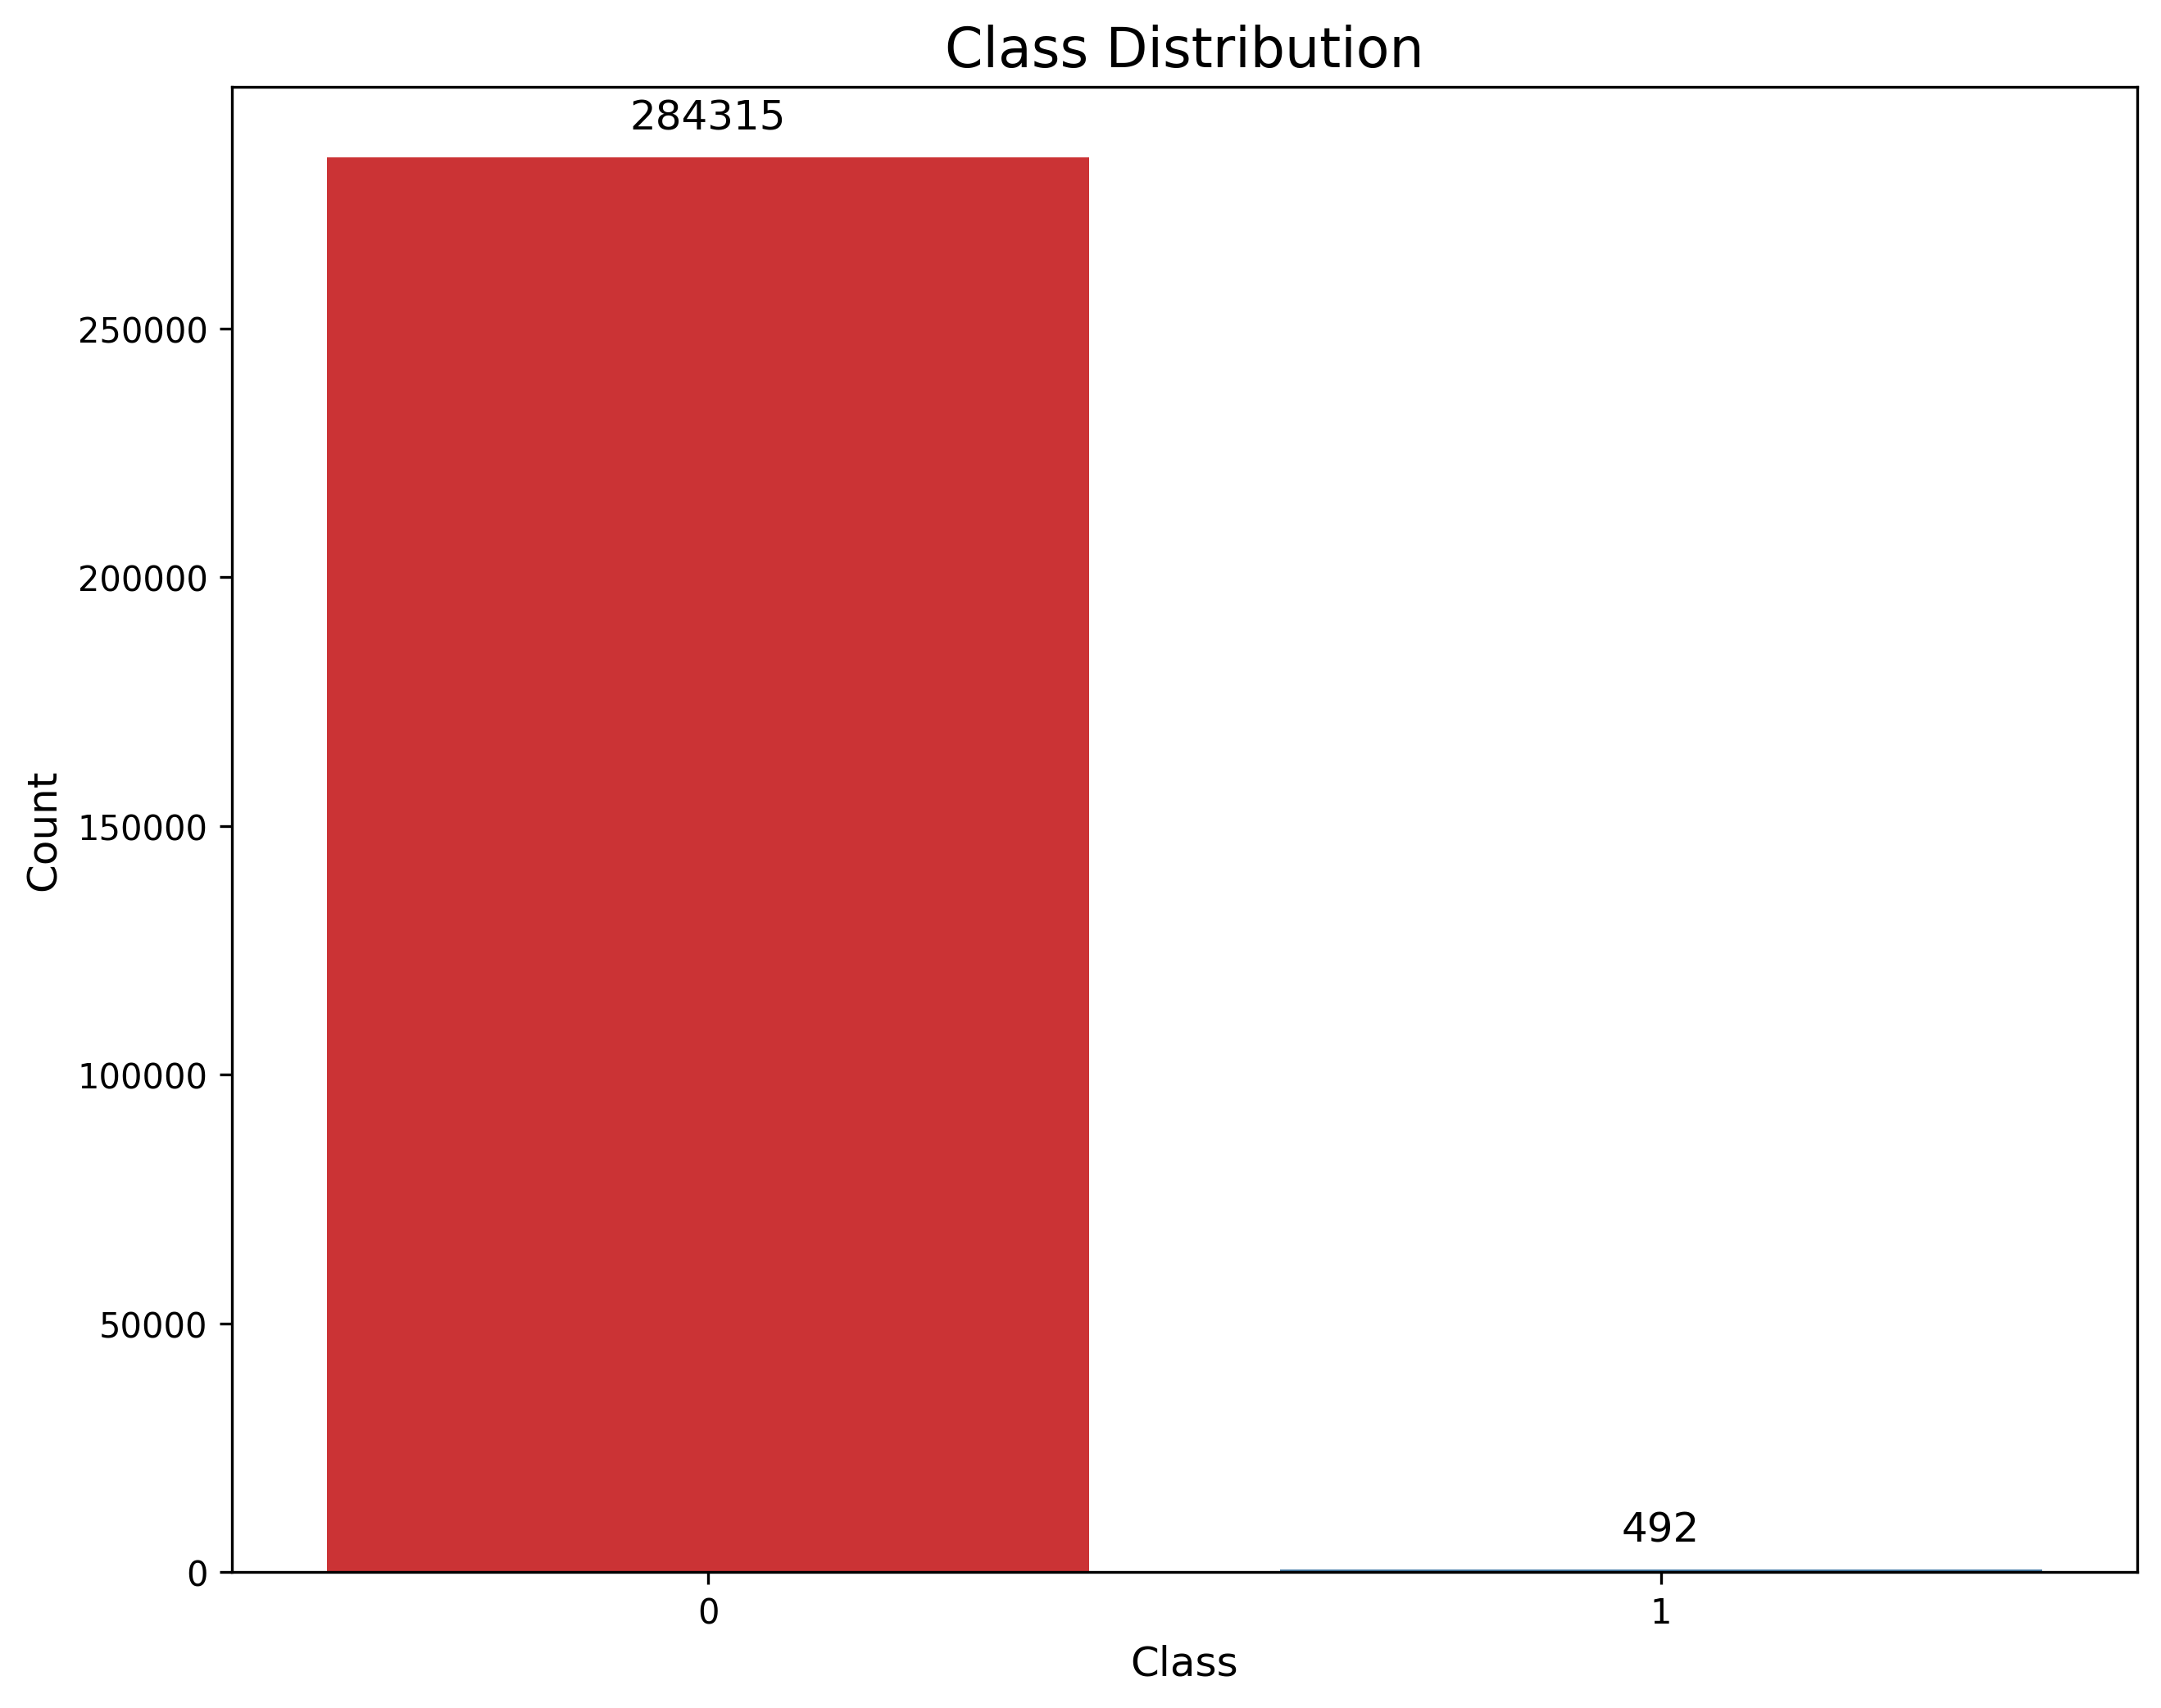
\includegraphics[width=0.8\textwidth]{images/class_distribution_before.png}
    \caption{Class Distribution Before SMOTE}
    \label{fig:class_distribution_before}
\end{figure}

\subsection{Data Splitting}

To simulate a real-world scenario and prevent data leakage, we sorted the data based on the \textbf{Time} feature and then split it into training and testing sets using a 70:30 ratio. This ensures that all transactions in the training set occur before those in the testing set, preserving the temporal order of transactions. By maintaining the chronological sequence, we mimic the real-time prediction of fraud in a production environment.

\subsection{Data Normalization}

Feature scaling is essential for many machine learning algorithms to ensure that all features contribute equally to the model's learning process. In our dataset, the \textbf{Time} and \textbf{Amount} features have different scales compared to the PCA-transformed features (\textbf{V1} to \textbf{V28}). To bring these features to a comparable scale, we standardized the \textbf{Time} and \textbf{Amount} features using the \textit{StandardScaler}. 

Standardization transforms each feature to have a mean of zero and a standard deviation of one. Crucially, this standardization was performed only after splitting the dataset into training and test sets. We first determined the scaling parameters using only the training data. Likewise, the test set was standardized independently. By treating the training and test sets independently, no information about the test distribution influences the training process. Otherwise, the model would indirectly gain insight into the test data’s distribution during training, inflating performance estimates in an unrealistic manner.

\subsection{Handling Imbalanced Data with SMOTE}

To address the severe class imbalance in the training data, we applied the SMOTE Technique. SMOTE generates synthetic samples for the minority class by interpolating between existing minority samples. We set the sampling strategy to achieve a 1:1 ratio between the majority and minority classes in the training set.

After applying SMOTE, the class distribution in the training set becomes balanced, as shown in Figure~\ref{fig:class_distribution_after}, while the test set remains unchanged to reflect real-world conditions.

\begin{figure}[H]
    \centering
    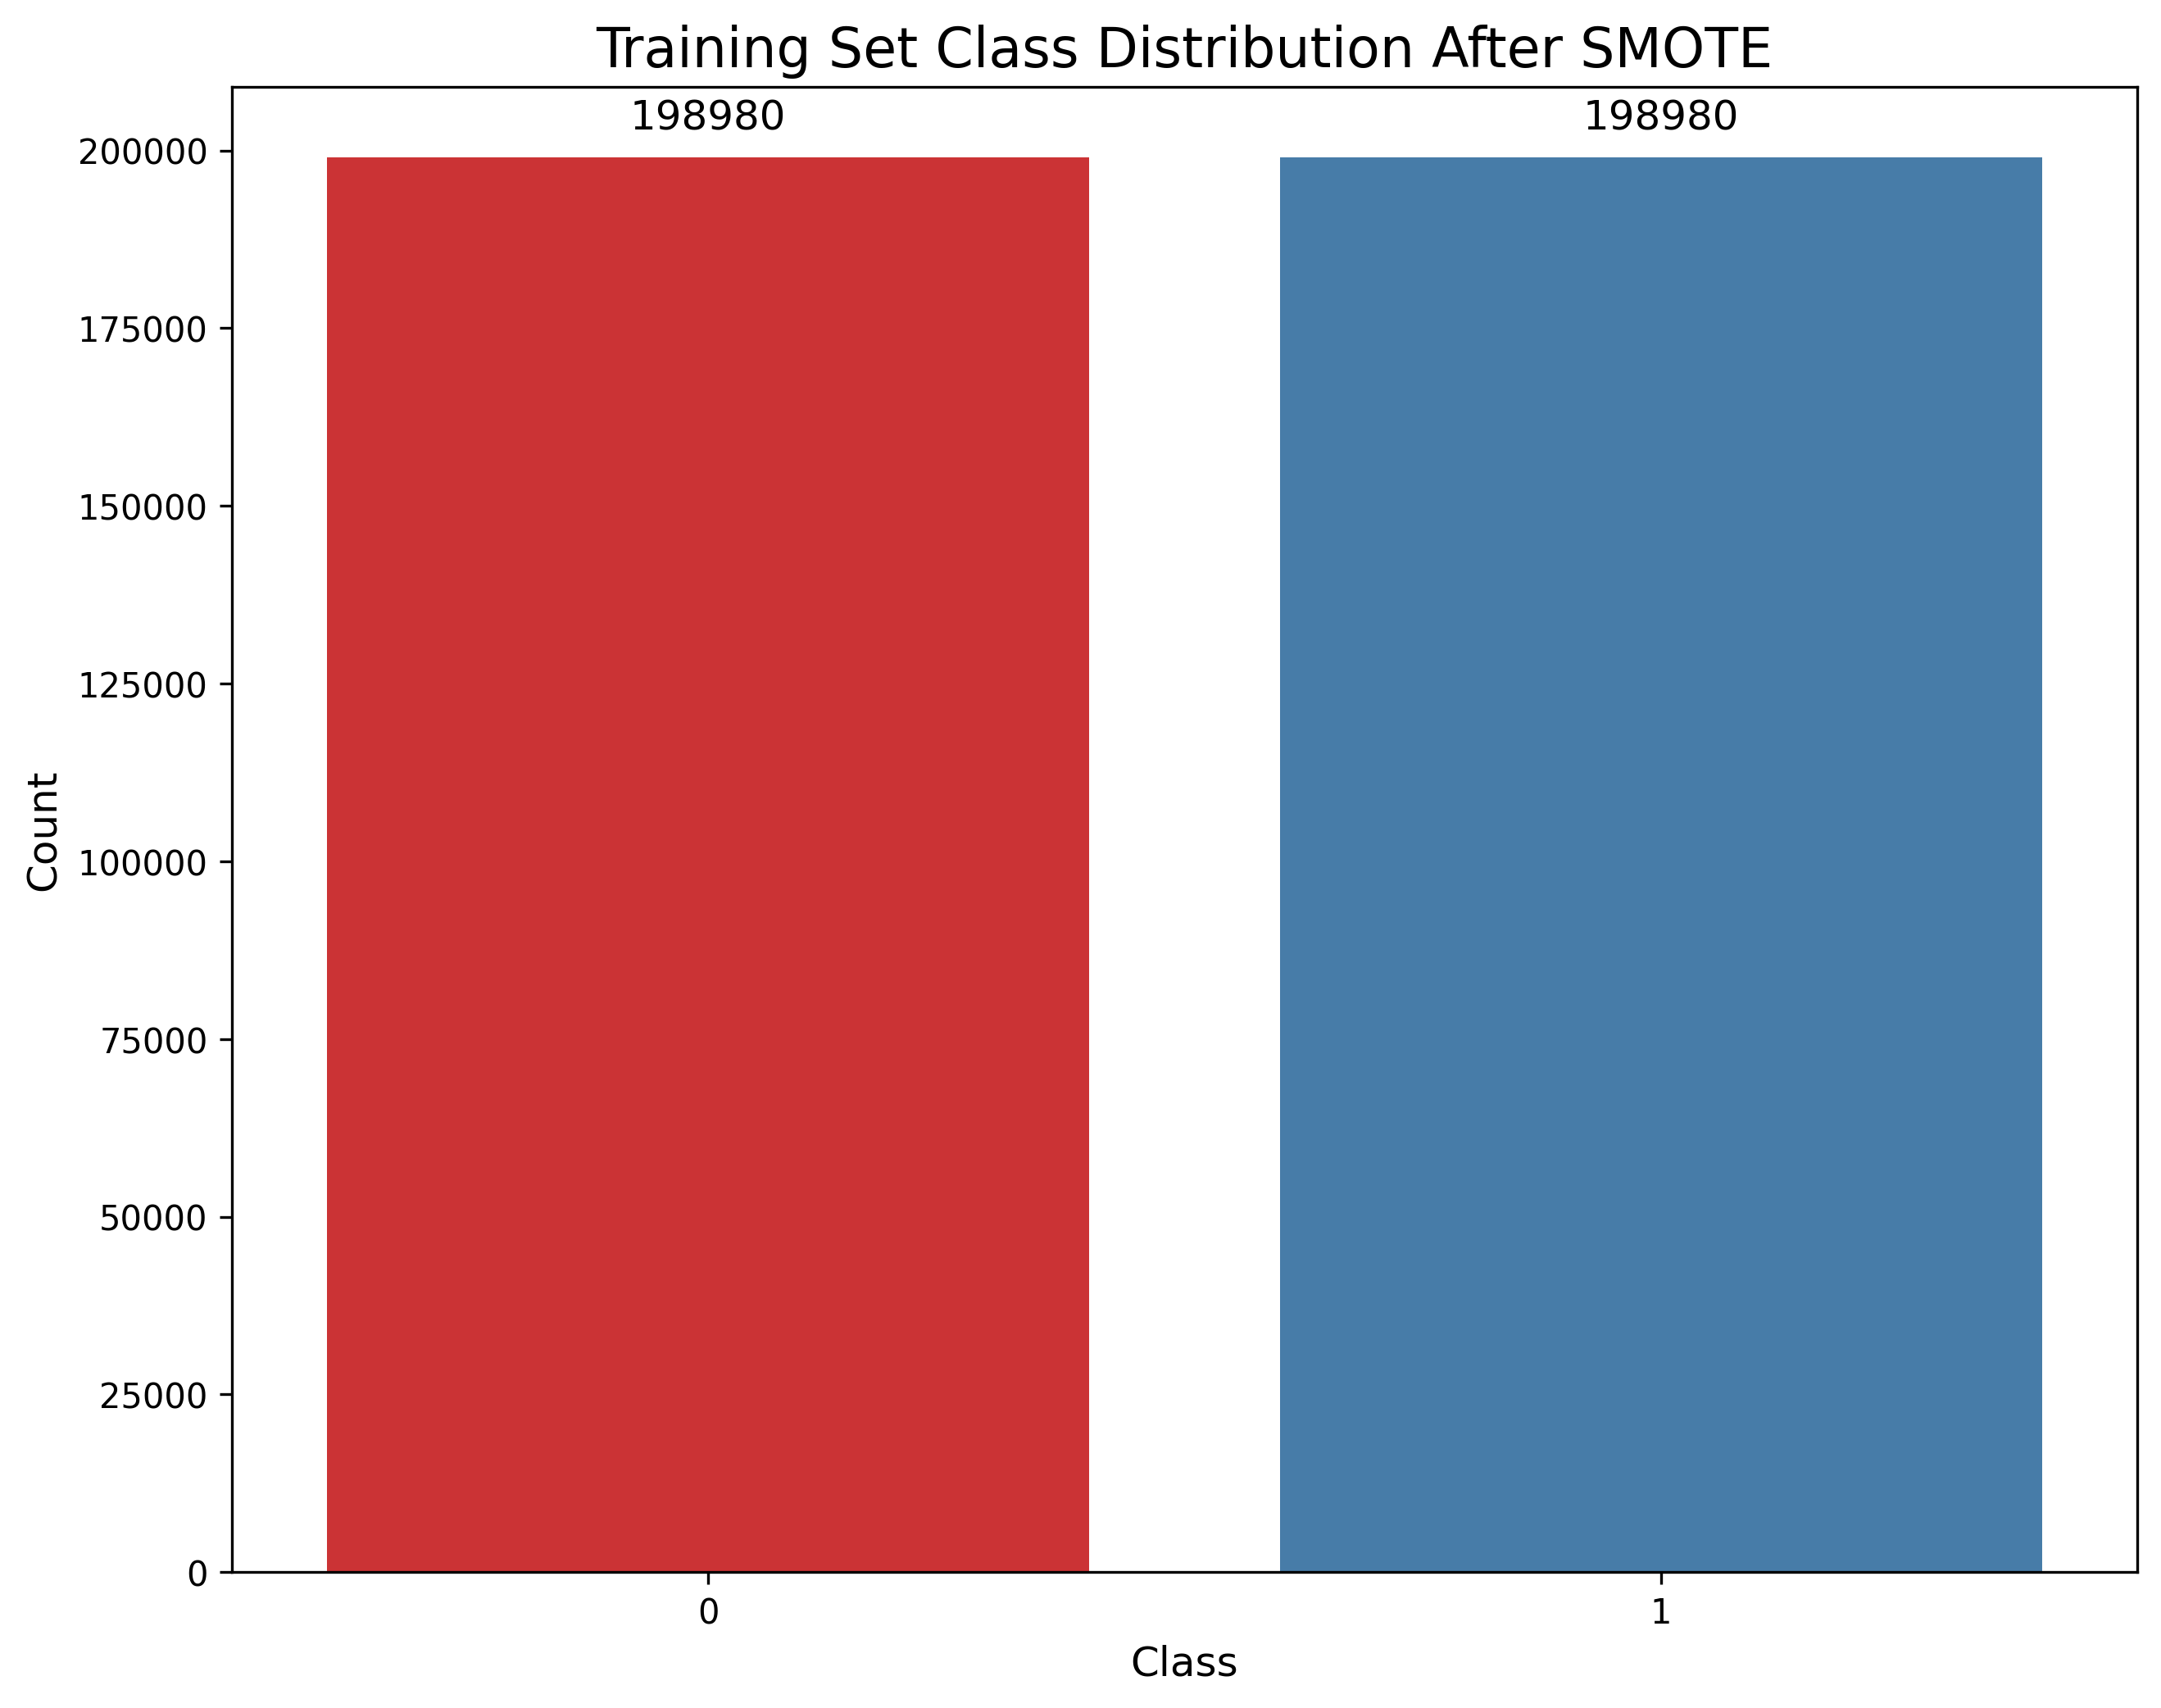
\includegraphics[width=0.8\textwidth]{images/class_distribution_after.png}
    \caption{Class Distribution After SMOTE}
    \label{fig:class_distribution_after}
\end{figure}

\subsection{Correlation Analysis}

We generated correlation heatmaps to investigate the relationships between features and the target variable both prior to and subsequent to applying SMOTE. In highly imbalanced datasets, the correlation coefficients can be misleading due to the scarcity of the minority class samples and the distorted data distribution. However, after applying SMOTE, as demonstrated in Figures~\ref{fig:correlation_before} and~\ref{fig:correlation_after}, the correlation between the \textbf{Class} variable and other features becomes more conspicuous.

SMOTE functions by generating synthetic samples of the minority class, thereby increasing its proportion and diversity within the dataset. This augmentation leads to a more balanced data distribution, allowing the relationships between features and the target variable to be more comprehensively represented in the correlation calculations. As a result, the enhanced correlations potentially assist the model in discerning distinctive patterns, which could otherwise be obscured in the presence of severe class imbalance.

\begin{figure}[H]
    \centering
    \begin{minipage}{0.49\textwidth}
        \centering
        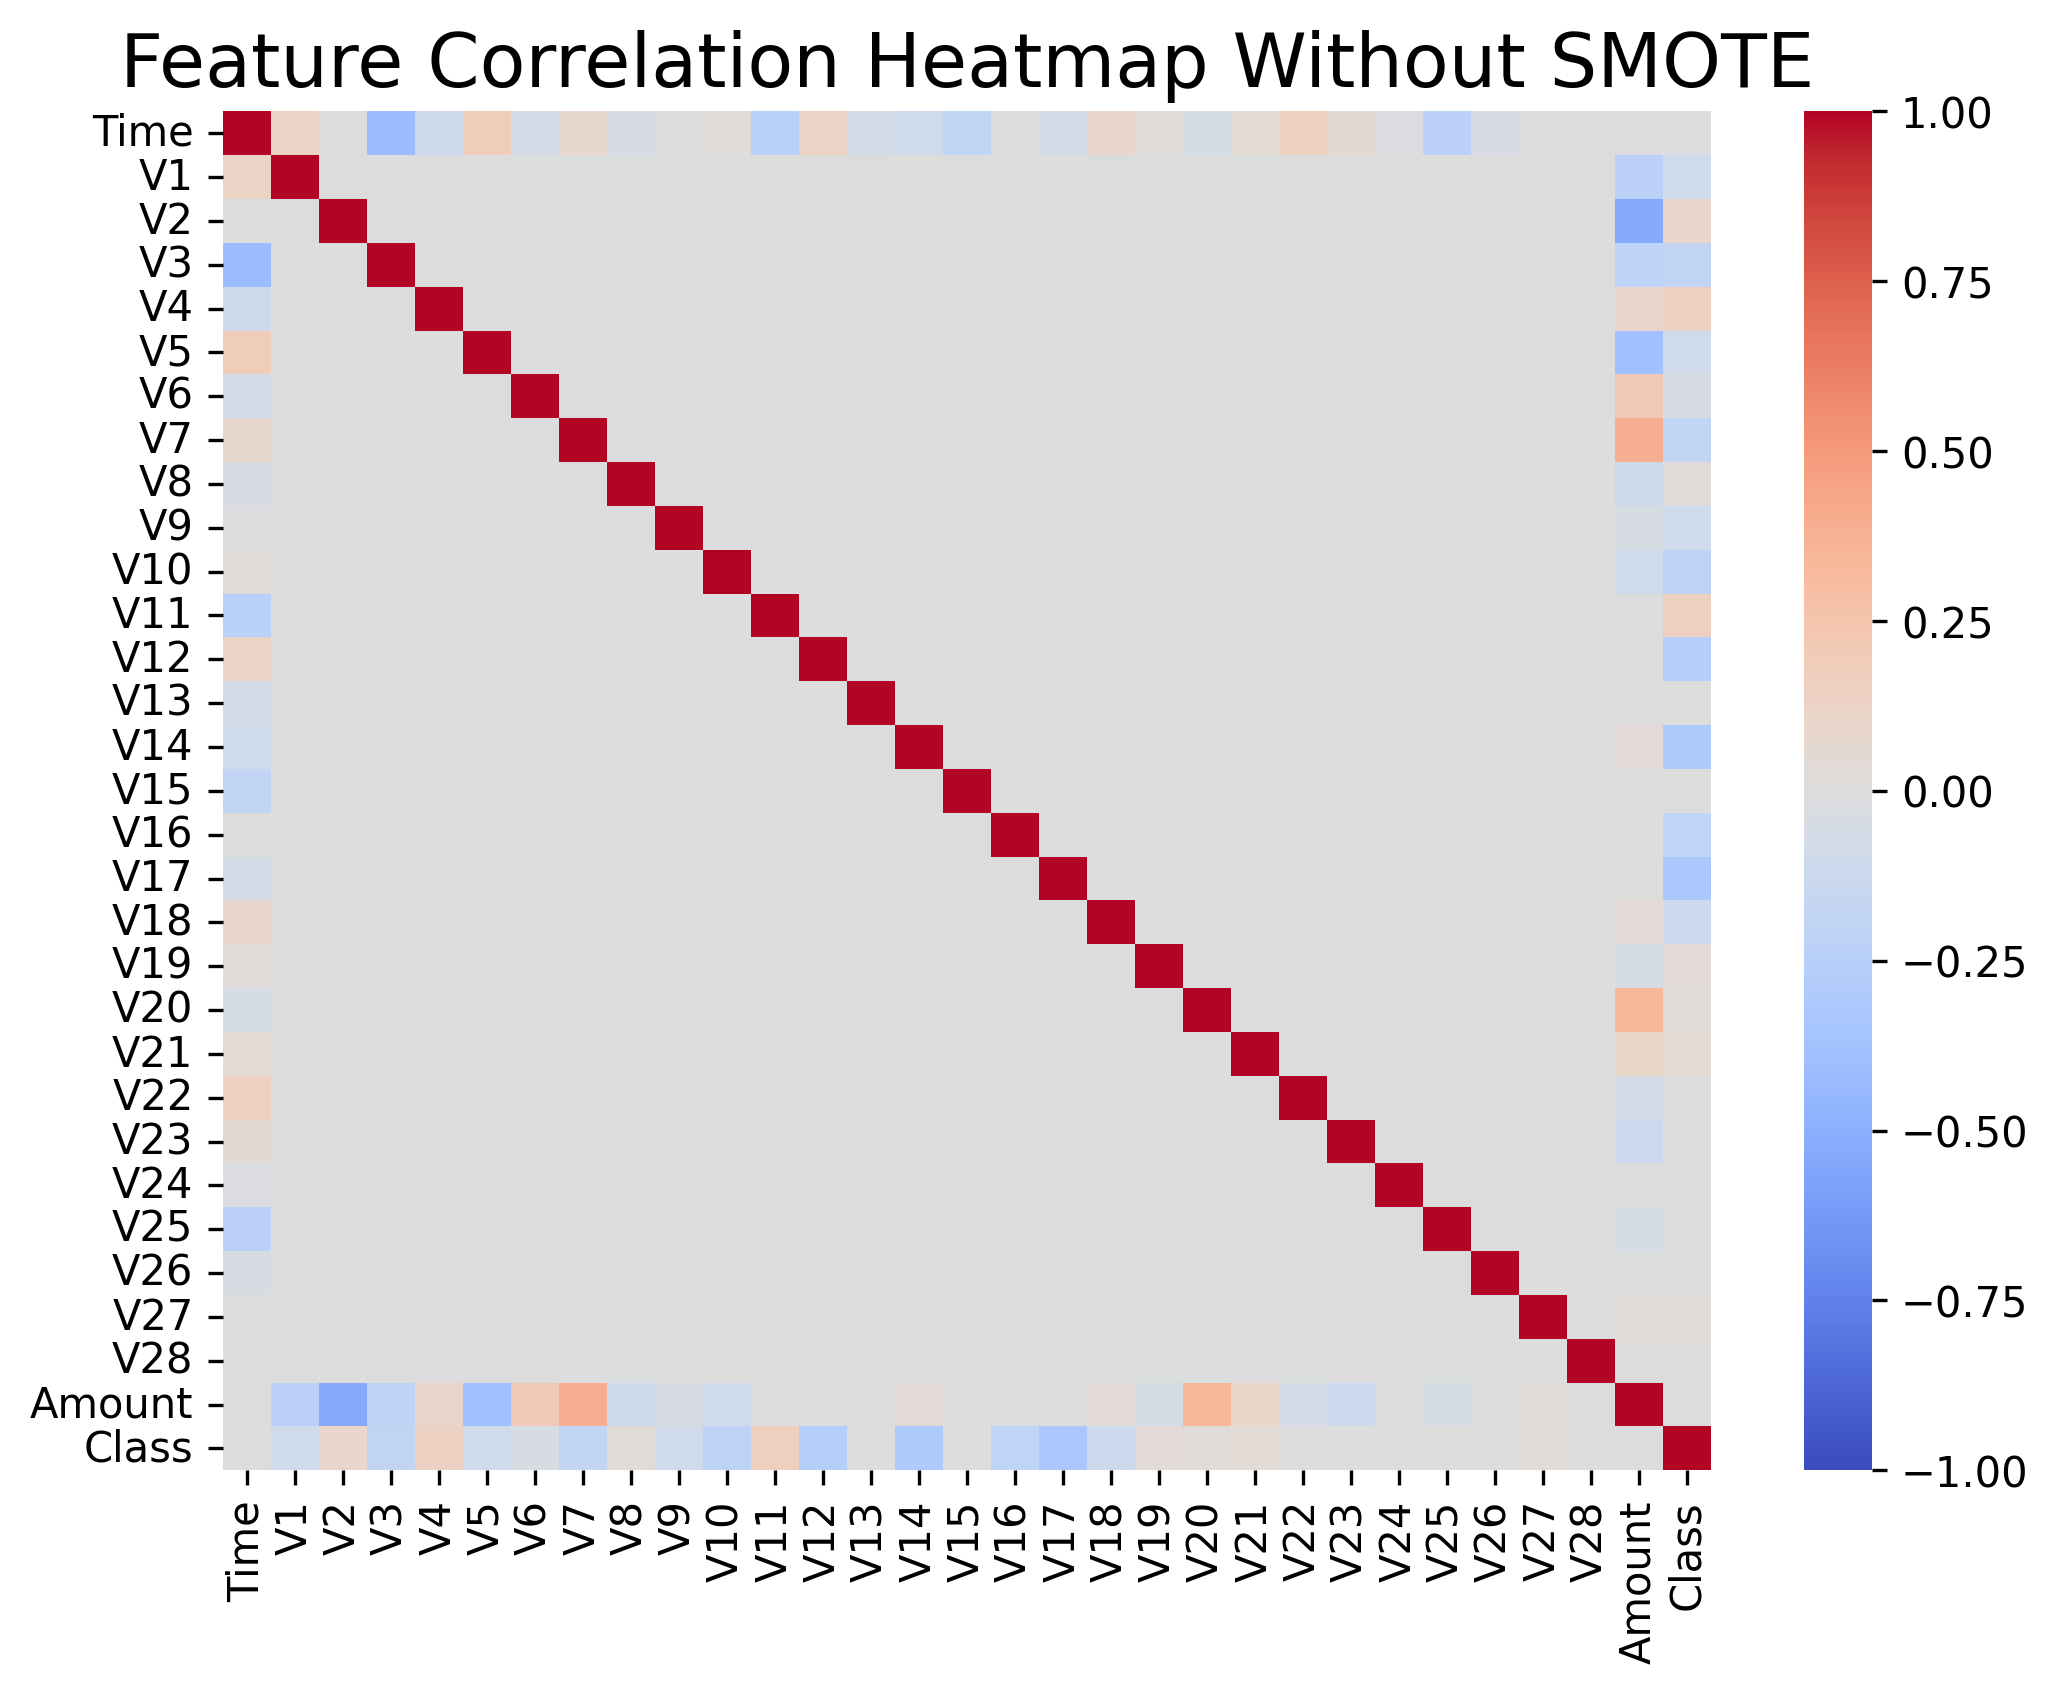
\includegraphics[width=1.0\textwidth]{images/correlation_before_smote.png}
        \caption{Correlation Heatmap Before SMOTE}
        \label{fig:correlation_before}
    \end{minipage}\hfill
    \begin{minipage}{0.49\textwidth}
        \centering
        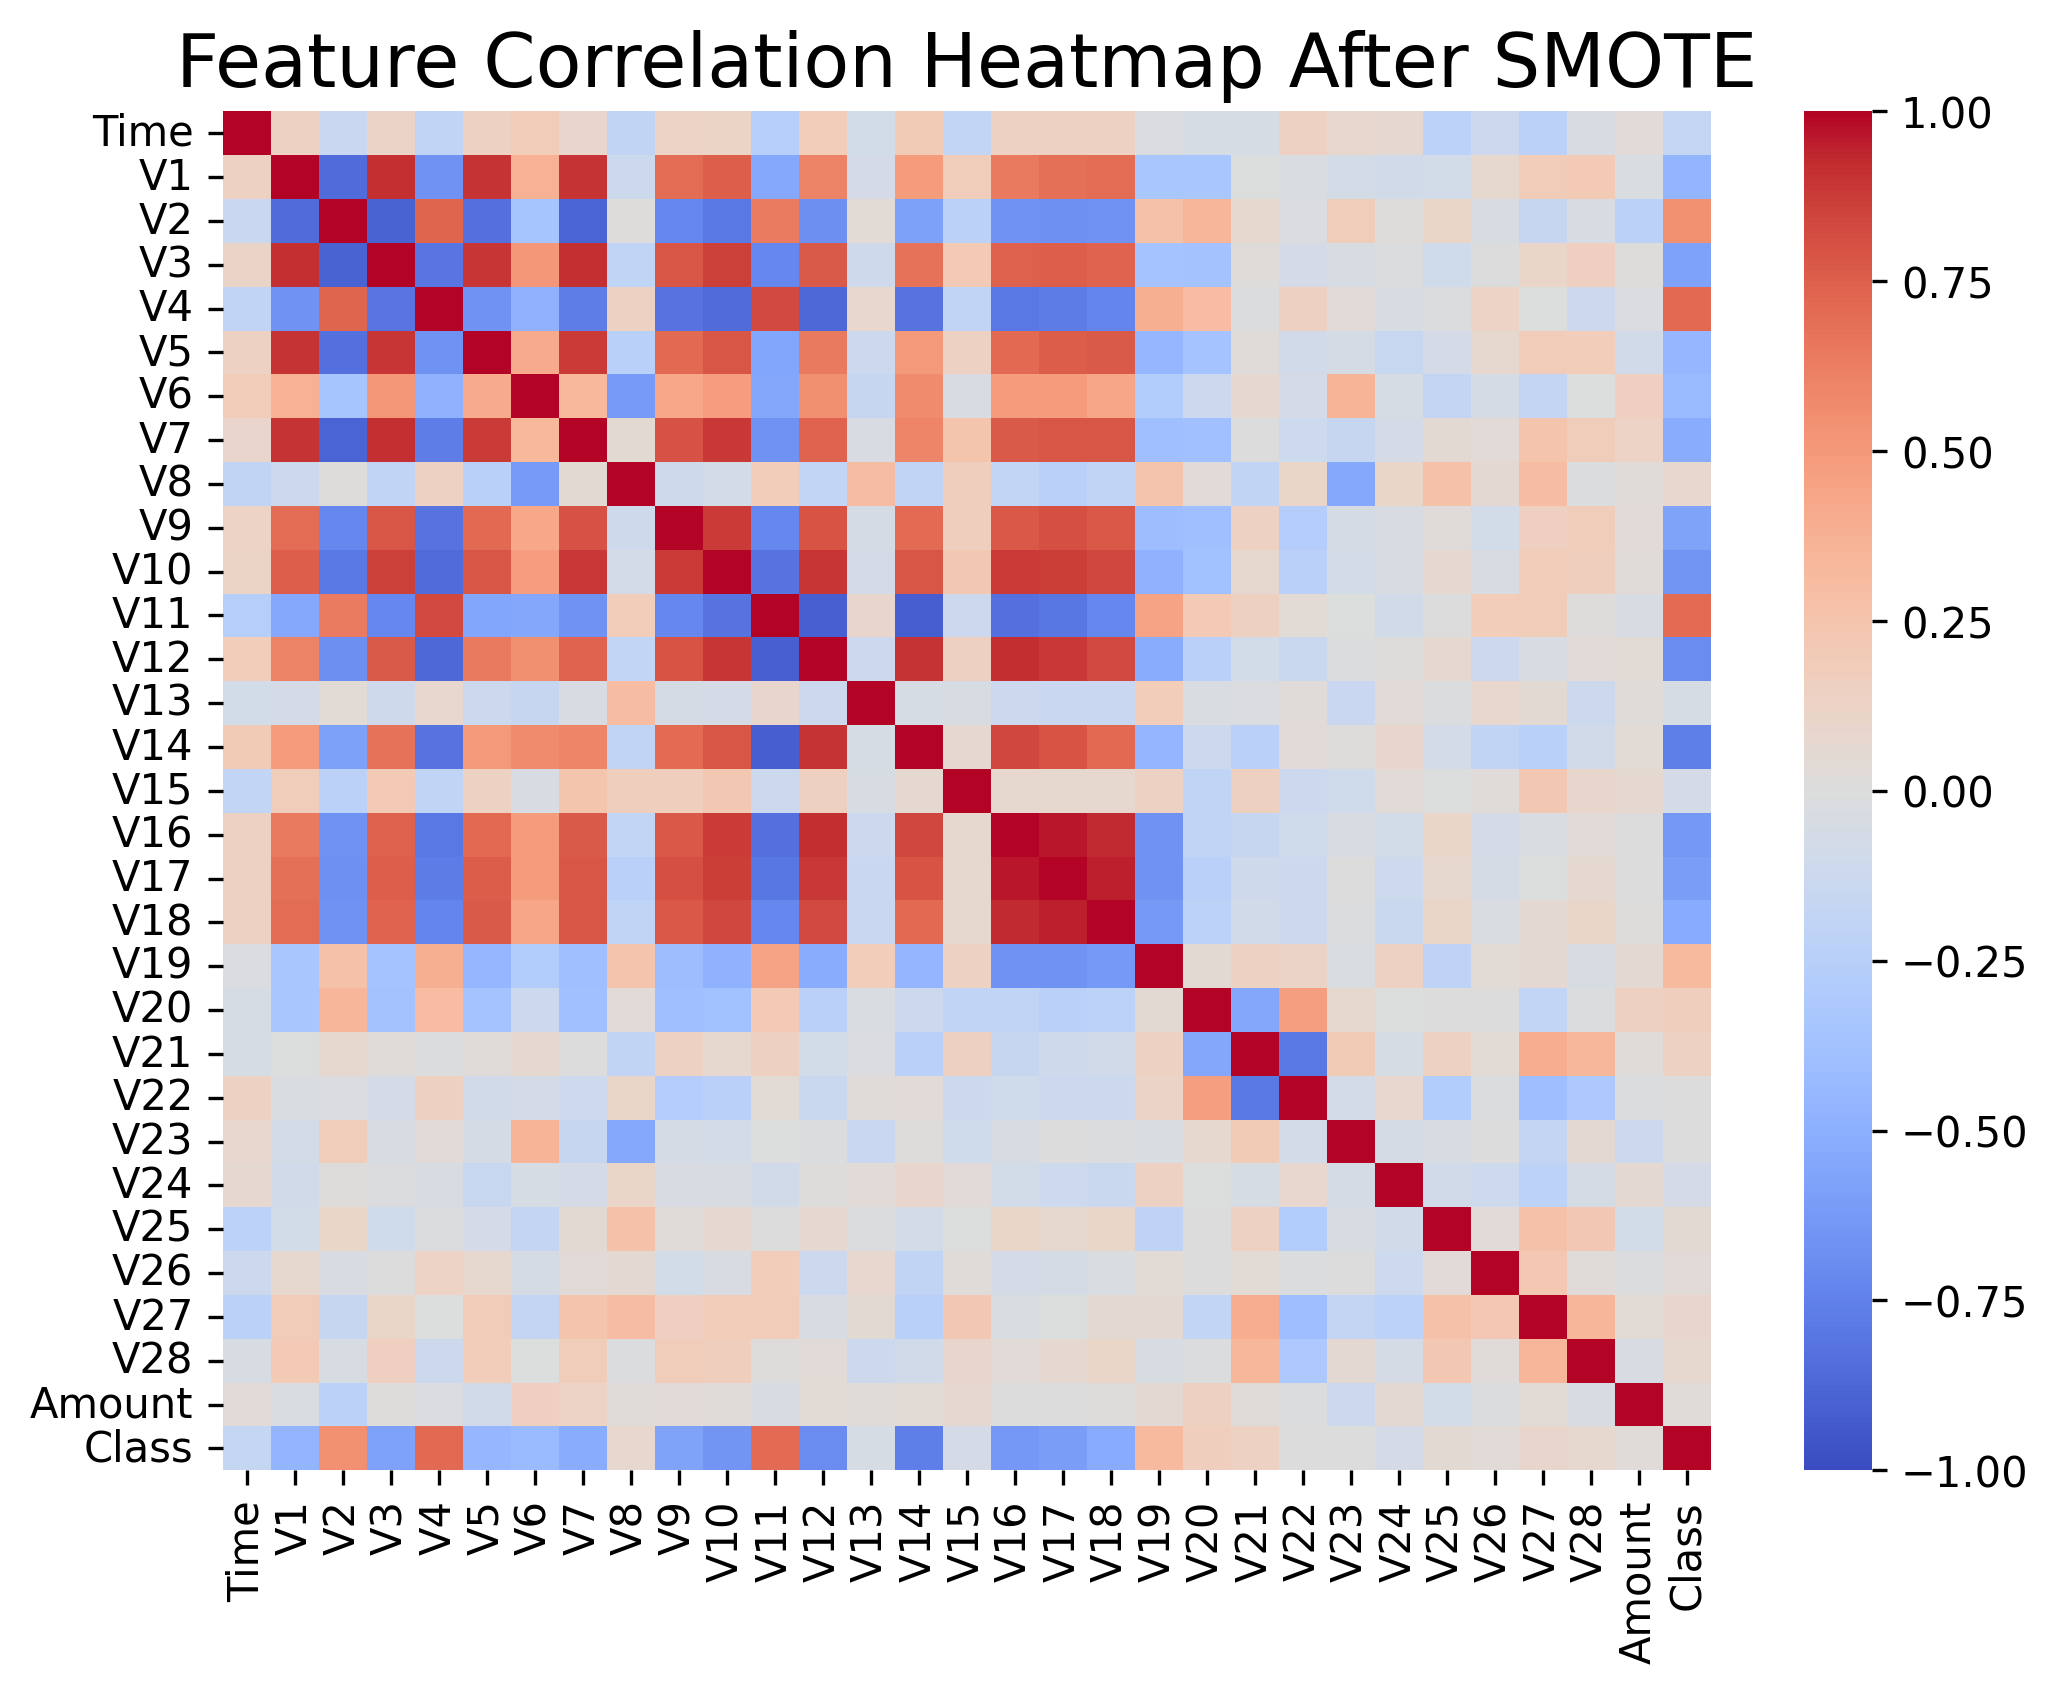
\includegraphics[width=1.0\textwidth]{images/correlation_after_smote.png}
        \caption{Correlation Heatmap After SMOTE}
        \label{fig:correlation_after}
    \end{minipage}
\end{figure}

\subsection{Data Preparation for Model Training}

After preprocessing, the data was prepared for model training. The resampled training data and the test data were converted into PyTorch tensors for deep learning models. Data loaders were created to facilitate efficient mini-batch processing during training.


\section{Methodology}

This section outlines the methodological framework employed in our study, encompassing both traditional machine learning models and advanced deep learning architectures. We begin by introducing baseline models that serve as reference points, and then progress to more sophisticated neural network structures. Additionally, we discuss the loss functions used to handle the severe class imbalance, as well as the evaluation metrics adopted for performance assessment.

\subsection{Baseline Models}

\subsubsection{Logistic Regression}

As a starting point, we employ a logistic regression model to establish a fundamental benchmark. This model is implemented using a single linear layer that maps the input features directly to a single output neuron, representing the predicted probability of fraud after applying a sigmoid activation function. Specifically, all preprocessed input features (including both the PCA-transformed variables and the standardized \textit{Time} and \textit{Amount}) are fed into a linear transformation of the form \(\mathbf{z} = \mathbf{W}\mathbf{x} + b\), where \(\mathbf{x}\) is the input vector, \(\mathbf{W}\) and \(b\) are learned parameters, and \(\mathbf{z}\) is the logit. A sigmoid function \(\sigma(z) = 1/(1 + e^{-z})\) then converts this logit into a probability between 0 and 1.

To optimize this model, we use the binary cross-entropy loss (BCELoss), which measures the discrepancy between predicted probabilities and true labels. We train the logistic regression model with the Adam optimizer at a learning rate of 0.001 for a fixed number of epochs (e.g., 30), iterating over the training data in mini-batches. This setup ensures a stable and relatively quick convergence. Although logistic regression does not inherently model complex interactions among features, it provides a clear, interpretable baseline for subsequent models.

\subsubsection{Random Forest}

As a second baseline, we utilize a random forest classifier with 100 decision trees. Each tree is trained on bootstrap samples of the balanced training data (obtained via SMOTE) and considers a random subset of features at each split. This approach helps capture non-linear relationships and interactions between features that logistic regression may miss. The model aggregates predictions from all trees through majority voting to produce the final classification. We do not rely on deep architecture or gradient-based optimization here; instead, we simply fit the random forest on the resampled training data and then obtain predictions for the test set. This baseline allows us to assess the benefits of ensemble methods and decision tree-based logic compared to linear models.

\subsection{Deep Learning Models}

\subsubsection{Multi-Layer Perceptron}

The MLP serves as a direct extension beyond linear models by stacking multiple layers and introducing non-linear activations. The architecture starts with an input layer corresponding to the dimensionality of the preprocessed features. It then includes intermediate hidden layers (one hidden layer with 128 neurons, followed by another with 64 neurons), each followed by a ReLU activation function to introduce non-linearity. To mitigate overfitting, dropout layers with a dropout rate (e.g., 0.3) are inserted after these hidden layers. Finally, the output layer consists of a single neuron with a sigmoid activation, producing a probability of fraud.

Just like logistic regression, the MLP is trained using BCELoss as the objective function and the Adam optimizer (learning rate 0.001). Training is conducted for a fixed number of epochs (e.g., 30), with mini-batches of data processed sequentially. The increased capacity of the MLP over logistic regression is expected to model more complex relationships among features, potentially improving recall and overall predictive performance.

\subsubsection{Long Short-Term Memory Network}

Although our dataset treats each transaction as an independent observation, we incorporate an LSTM model to explore the potential benefits of sequence modeling. The LSTM architecture includes multiple layers (e.g., two LSTM layers) with a hidden dimension of 64. Each transaction vector is processed as a single time step, effectively treating our input as sequences of length one. While this does not fully exploit temporal patterns (as we are not grouping multiple transactions into longer sequences), the LSTM architecture still demonstrates how recurrent layers can be integrated.

Within the LSTM, memory cells and gating mechanisms regulate the flow of information. After passing through the recurrent layers, the last hidden state is fed into a fully connected layer, followed by a sigmoid activation, to produce the fraud probability. We optimize this model similarly to the MLP, using BCELoss and the Adam optimizer at a 0.001 learning rate. Even though the benefit of LSTMs may be limited by the lack of extended sequential context in the current setup, this model still provides insight into how recurrent architectures behave in this domain.

\subsubsection{Transformer-Based Model}

While LSTMs rely on sequential processing, the Transformer-based model employs a self-attention mechanism to capture relationships between features without strictly following a temporal order. We first project the input feature vector into a higher-dimensional representation (e.g., embedding dimension of 256) through a linear embedding layer, followed by dropout (e.g., 0.3) for regularization. The core of the Transformer model is a stack of encoder layers, each consisting of multi-head self-attention and position-wise feed-forward networks. In our implementation, we employ two encoder layers with four attention heads.

\begin{figure}[H]
    \centering
    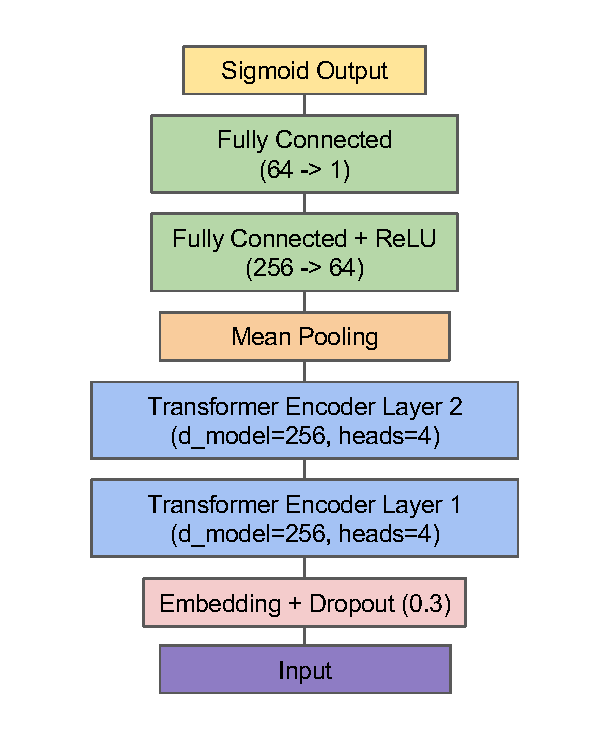
\includegraphics[width=0.5\textwidth]{images/transformer_architecture.pdf}
    \caption{An overview of the Transformer-based model architecture for fraud detection}
    \label{fig:transformer_arch}
\end{figure}

The self-attention mechanism computes attention weights between all positions in the input. If the input consists of a single vector (a single “time step”), this reduces the complexity of attention calculations, but the architecture can readily handle sequences if the data were organized as such. When sequences are longer, the Transformer captures long-range dependencies by allowing any position to attend to any other, rather than being constrained by recurrence as in LSTMs.

Following the encoder layers, we aggregate the transformed representations via a simple mean pooling over the sequence dimension. This pooled representation is then fed into a small fully connected network with a hidden dimension (e.g., 64) and a ReLU activation before producing a final fraud probability through a sigmoid layer. The model is trained using BCELoss or, in some configurations, a Focal Loss to tackle class imbalance more effectively.

For optimization, we use the AdamW optimizer with a learning rate of 0.001 and a weight decay for regularization. A learning rate scheduler (e.g., ReduceLROnPlateau) monitors the training loss and reduces the learning rate if progress stalls. The Transformer architecture, by design, can handle more complex and potentially longer patterns if provided with sequential data. Although our current setup treats each transaction independently, this architecture provides a flexible and scalable framework that can be adapted if temporal or sequential structuring of transactions becomes relevant.

\subsection{Loss Functions}

\subsubsection{Binary Cross-Entropy (BCE) Loss}

Binary Cross-Entropy loss is a standard objective for binary classification tasks. For a single instance with a true label \( y \in \{0,1\} \) and predicted probability \( p \), the BCE loss is defined as:

\[
L_{\text{BCE}}(p, y) = -\bigl[\,y \log(p) + (1 - y)\log(1 - p)\bigr]
\]

BCE loss treats both classes equally and does not inherently address class imbalance. In highly skewed datasets, this may lead the model to be biased towards the majority class since misclassifying rare positive examples does not sufficiently increase the overall loss.

\subsubsection{Focal Loss}

Focal Loss is designed to tackle imbalanced classification problems by modifying the standard BCE loss. It introduces a focusing parameter \(\gamma \geq 0\) that places more emphasis on hard-to-classify examples. Additionally, an \(\alpha \in [0,1]\) parameter is included to balance the relative importance of positive and negative classes. For a single instance, the Focal Loss can be written as:

\[
L_{\text{focal}}(p, y) = - \bigl[\alpha y(1 - p)^\gamma \log(p) + (1 - \alpha) (1 - y) p^\gamma \log(1 - p)\bigr]
\]

Here:
\begin{itemize}
    \item \(\alpha\) controls the class weighting. Setting \(\alpha = 0.5\) assigns equal weight to both classes.
    \item \(\gamma\) modulates the relative importance of correctly classified vs. misclassified samples. Larger \(\gamma\) values increase the emphasis on hard (misclassified) examples.
\end{itemize}

It is noteworthy that when \(\alpha = 0.5\) and \(\gamma = 0\), the Focal Loss reduces to a scaled version of BCE Loss:

\[
L_{\text{focal}}(p,y) \xrightarrow[\alpha=0.5,\gamma=0]{} -0.5 \bigl[y \log(p) + (1 - y)\log(1 - p)\bigr].
\]

\subsection{Evaluation Metrics}

To assess model performance, we employ \textbf{Recall} and the \textbf{ROC AUC Score}. Recall measures the proportion of actual fraud cases correctly identified, which is crucial in minimizing missed fraud. The ROC AUC Score evaluates the model’s ability to rank positive instances higher than negative ones across varying classification thresholds, providing a holistic measure of the model's discriminative power.

By relying on these metrics, we ensure that our evaluation criteria reflect the real-world priority of identifying as many fraudulent transactions as possible without overly inflating performance due to the majority of non-fraudulent examples.

\subsection{Summary}
Here is the summary of the models employed in our study. Key aspects such as the architectures and training parameters are presented in Tables \ref{table:model_params_arch} and \ref{table:model_params_train} respectively for a clear comparison.

\begin{table}[H]
\centering
\caption{Models and Their Architectures}
\label{table:model_params_arch}
\begin{tabular}{lcp{3.85cm}c}
\hline
\textbf{Model} & \textbf{Architecture} & \textbf{Key Layers} \\ \hline
\textbf{Logistic Regression} & Single linear layer + sigmoid & Input dim $\rightarrow$ 1 \\[4pt]
\textbf{Random Forest} & Ensemble of 100 trees & n\_estimators = 100 \\[4pt]
\textbf{MLP} & Fully connected network & fc1: 128; fc2: 64 \\[4pt]
\textbf{LSTM} & 2-layer LSTM + linear output & hidden\_dim: 64; \newline num\_layers: 2 \\[4pt]
\textbf{Transformer} & 2-layer encoder; multi-head attention & d\_model: 256; heads: 4 \\ \hline
\end{tabular}
\end{table}

\begin{table}[H]
\centering
\caption{Models' Training Parameters}
\label{table:model_params_train}
\begin{tabular}{lcccc}
\hline
\textbf{Model} & \textbf{Loss} & \textbf{Optimizer} & \textbf{Learning Rate} & \textbf{Epochs} \\ \hline
\textbf{Logistic Regression} & BCE & Adam & 0.001 & 30 \\[4pt]
\textbf{Random Forest} & N/A & N/A & N/A & N/A \\[4pt]
\textbf{MLP} & BCE & Adam & 0.001 & 30 \\[4pt]
\textbf{LSTM} & BCE or Focal & Adam & 0.001 & 30 \\[4pt]
\textbf{Transformer} & BCE or Focal & AdamW & 0.001 & 30 \\ \hline
\end{tabular}
\end{table}


\section{Experiments and Results}

This section presents a comprehensive evaluation of our models under various experimental settings. We first examine the impact of SMOTE on a baseline Logistic Regression model. We then compare the performance of different models trained with BCELoss, followed by an investigation into the effect of Focal Loss with varying \(\gamma\) values. Finally, we discuss why the performance of the Transformer model is comparable to that of Logistic Regression, despite the former's complexity.

\subsection{Effect of SMOTE on Logistic Regression}

To demonstrate the necessity of addressing class imbalance, we begin with a Logistic Regression model, evaluating its performance both with and without SMOTE. Without SMOTE, the dataset remains highly imbalanced, resulting in a model that, while achieving near-perfect accuracy, fails to adequately capture the minority class. After applying SMOTE to the training set, the class distribution is balanced, encouraging the model to focus more on the minority class.

Table~\ref{tab:lr_smote} summarizes the performance of Logistic Regression before and after SMOTE. We report \textbf{Recall} and \textbf{ROC AUC Score}, as these metrics are more informative than accuracy for highly imbalanced problems. Figures~\ref{fig:confusion_matrix_lr_without_smote} and \ref{fig:confusion_matrix_lr_with_smote} illustrate the confusion matrices for the Logistic Regression model before and after SMOTE, respectively.

\begin{table}[H]
\centering
\caption{Performance of Logistic Regression With and Without SMOTE}
\label{tab:lr_smote}
\begin{tabular}{lcccc}
\hline
 & Accuracy & Recall (Fraud) & ROC AUC Score\\
\hline
Without SMOTE & 1.00 & 0.60 & 0.80 \\
With SMOTE    & 0.97 & 0.90 & 0.93 \\
\hline
\end{tabular}
\end{table}

Before SMOTE, the model easily identifies the majority class (non-fraud) but struggles with the minority class. Although accuracy is deceptively high, the recall for fraud cases is limited, underscoring the importance of metrics beyond accuracy. After applying SMOTE, the recall and ROC AUC Score improve notably, indicating a heightened sensitivity to fraudulent transactions at the expense of some false positives among the non-fraudulent cases. This trade-off is acceptable in fraud detection scenarios, where identifying rare positive cases is paramount.

The confusion matrices (as shown in the Figures~\ref{fig:confusion_matrix_lr_without_smote} and \ref{fig:confusion_matrix_lr_with_smote}) further confirm that after SMOTE, the model recognizes more fraudulent instances, albeit at the cost of classifying some legitimate transactions as fraud.

\begin{figure}[H]
    \centering
    \begin{minipage}{0.49\textwidth}
        \centering
        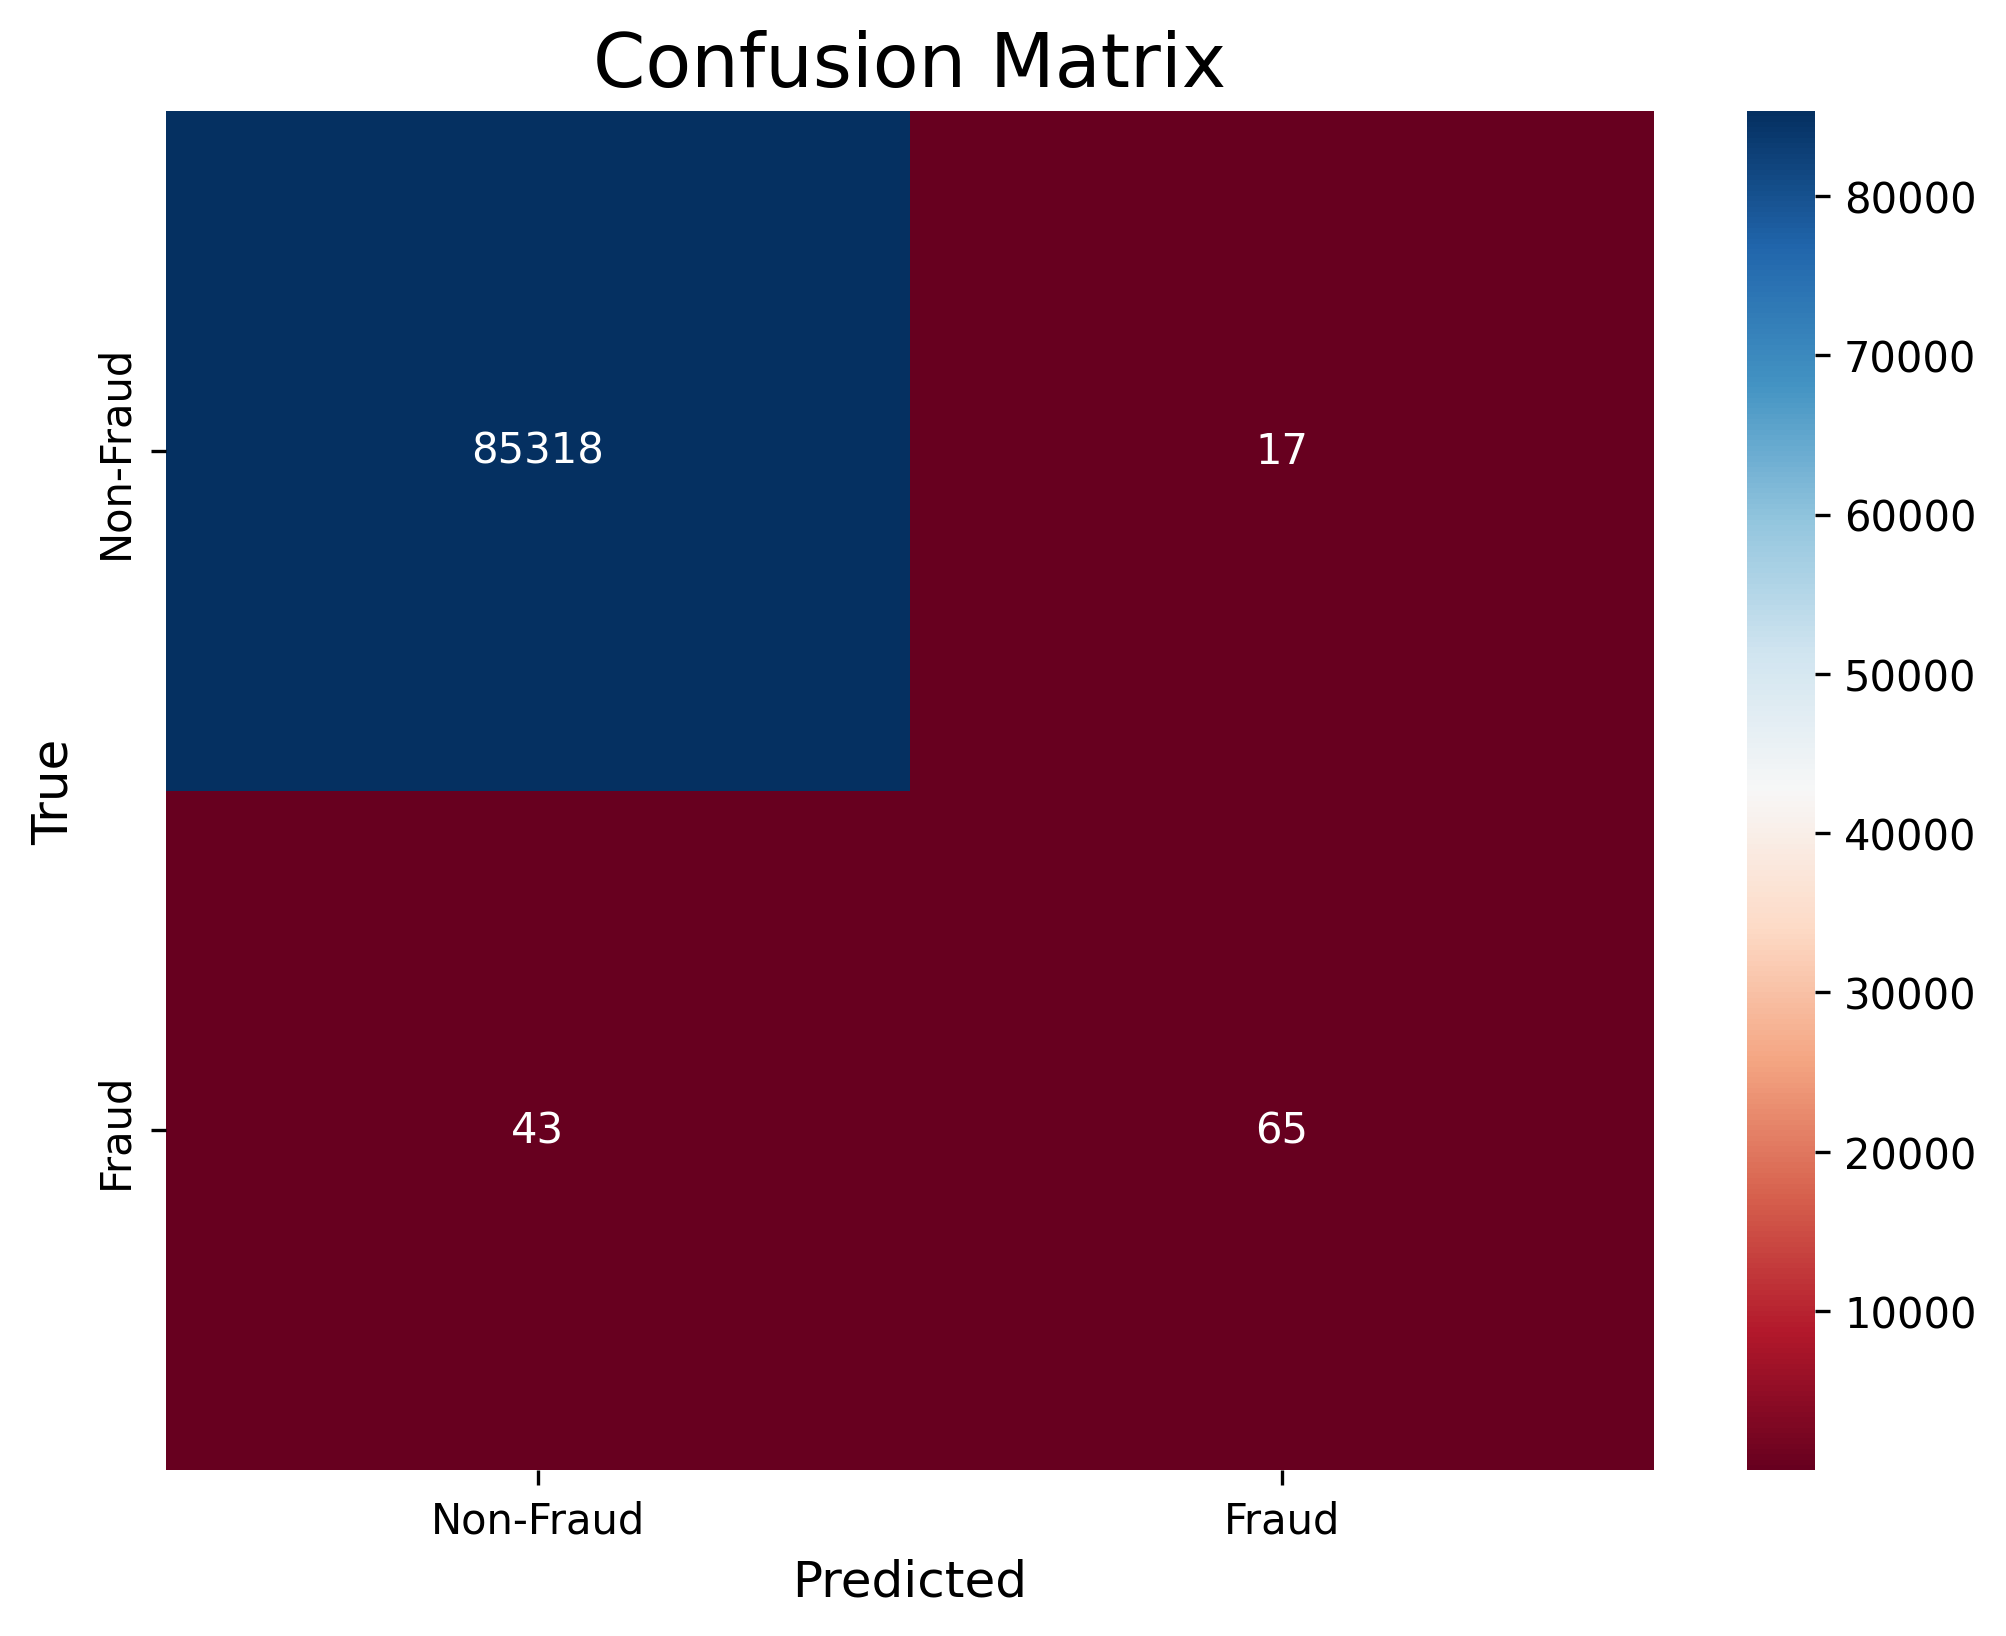
\includegraphics[width=1.0\textwidth]{images/confusion_matrix_logit_without_smote.png}
        \caption{Confusion Matrix for Logistic Regression Without SMOTE}
        \label{fig:confusion_matrix_lr_without_smote}
    \end{minipage}\hfill
    \begin{minipage}{0.49\textwidth}
        \centering
        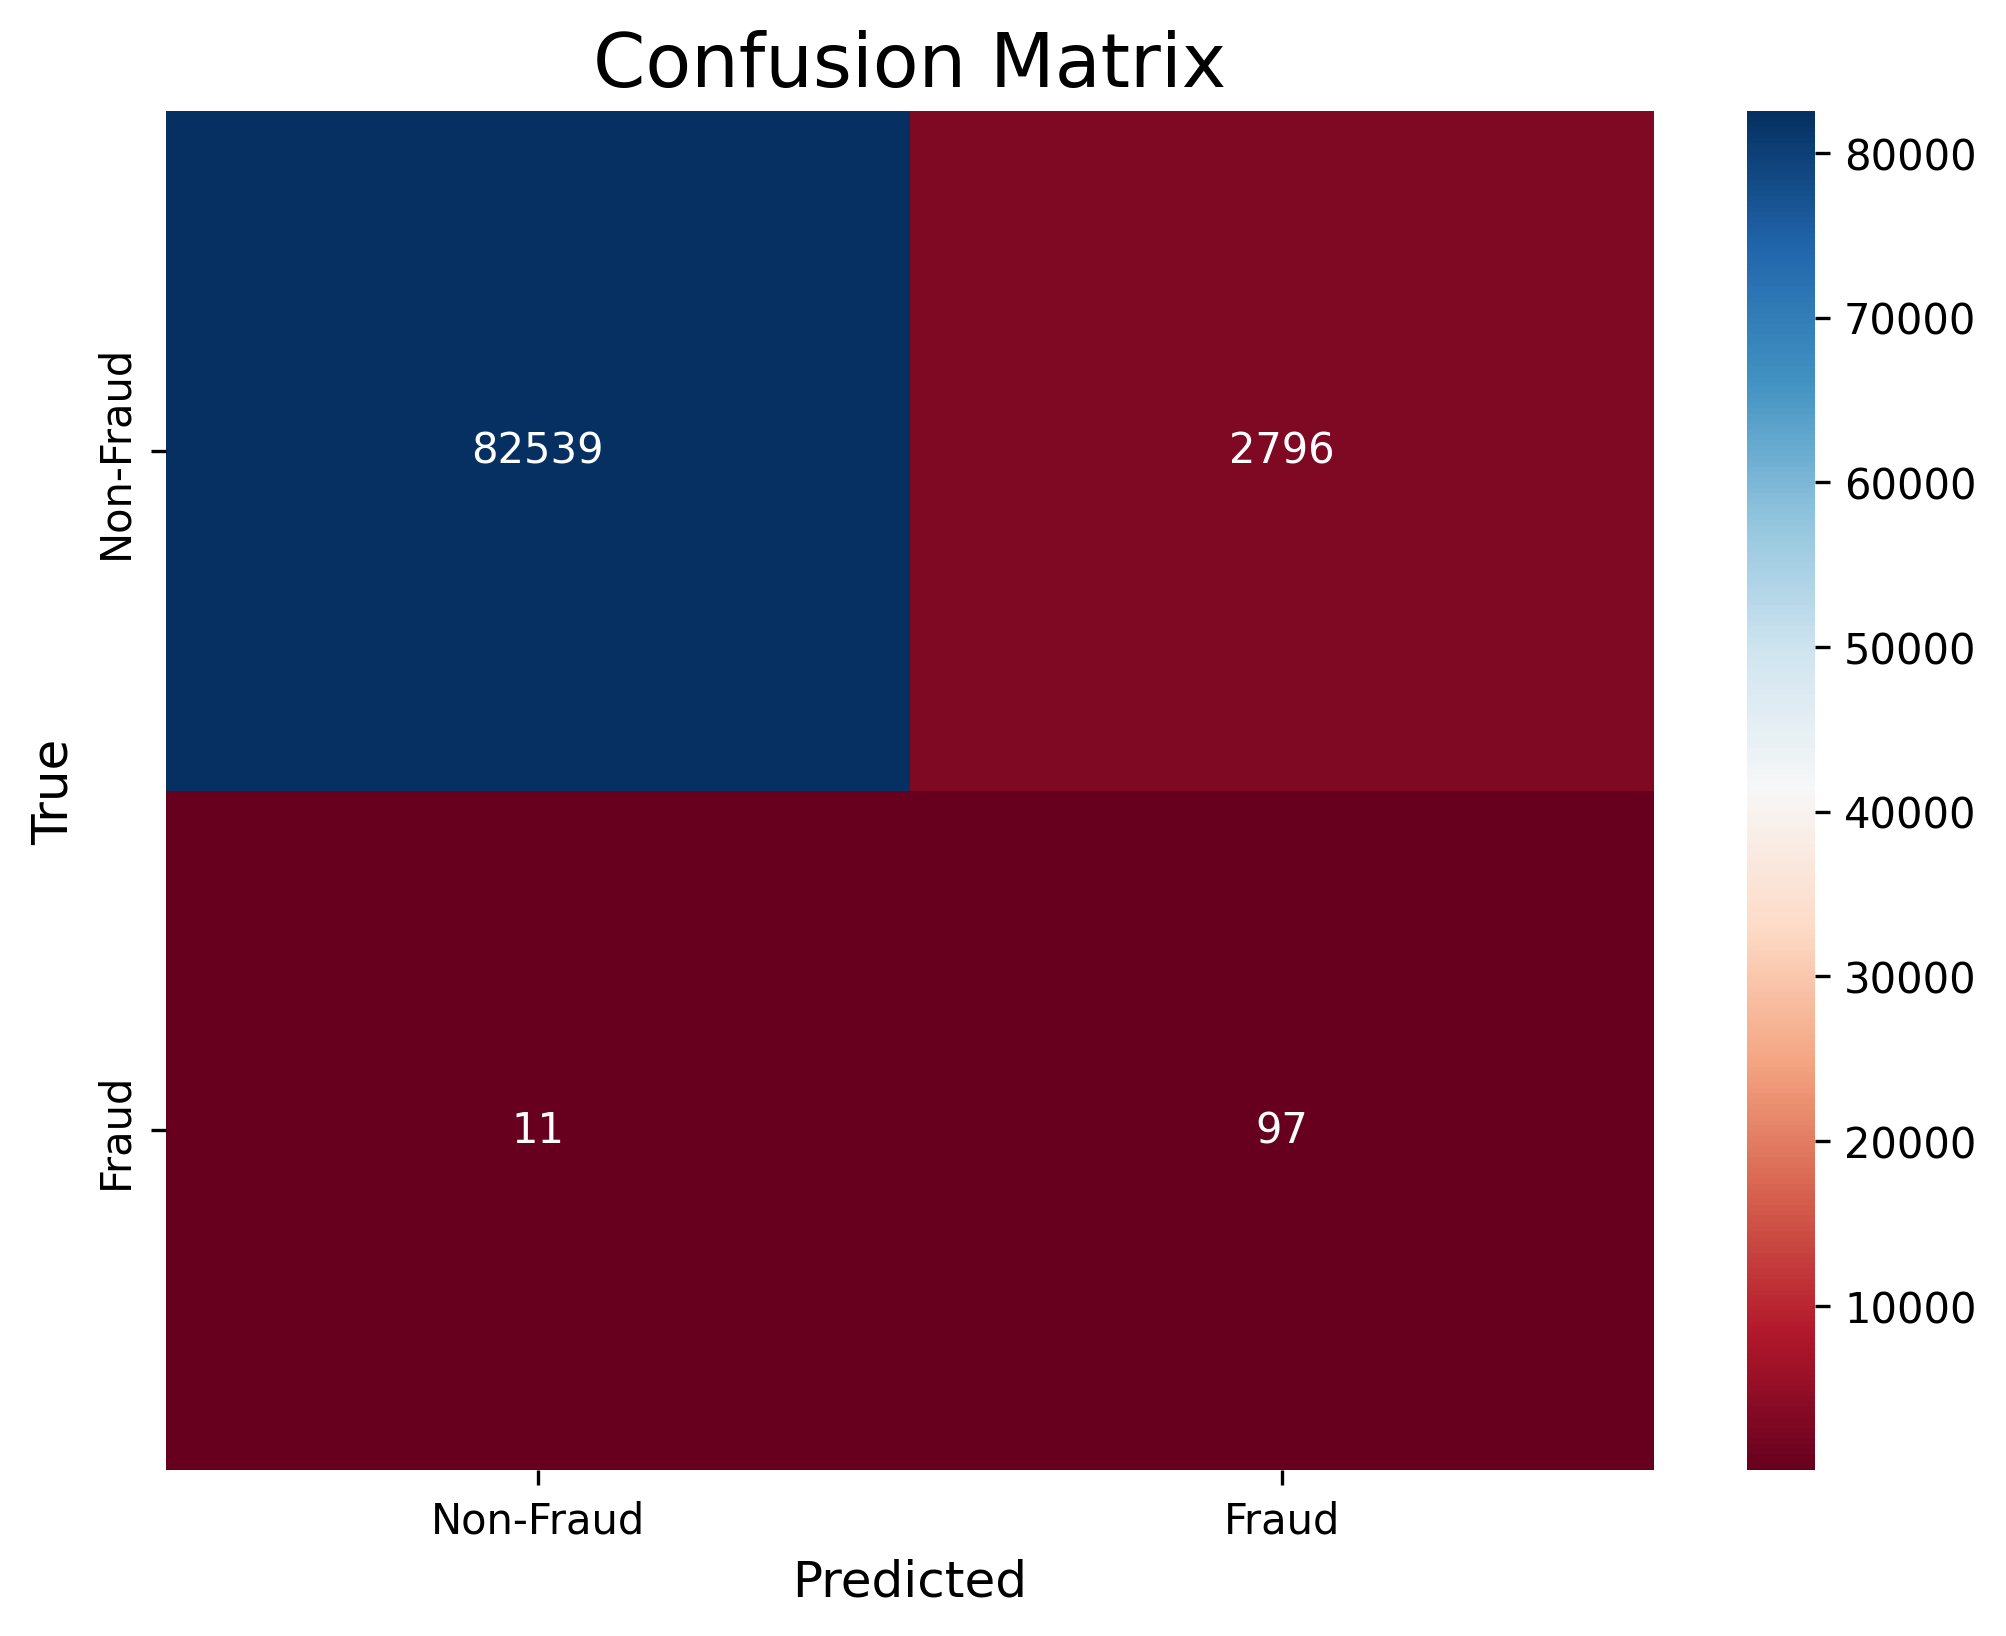
\includegraphics[width=1.0\textwidth]{images/confusion_matrix_logit.png}
        \caption{Confusion Matrix for Logistic Regression After SMOTE}
        \label{fig:confusion_matrix_lr_with_smote}
    \end{minipage}
\end{figure}


\subsection{Model Performance Comparison}

After establishing the importance of SMOTE, we train and evaluate Random Forest, LSTM, MLP, and Transformer models, all using BCELoss on the SMOTE-balanced training set. Each model’s configuration (as previously described in the Methodology) aims to capture different types of patterns—ranging from simple linear decision boundaries (Logistic Regression) to complex non-linear interactions (Random Forest, MLP) and temporal or sequence-like structures (LSTM, Transformer).

To visualize the results, we present a summary of their performance metrics in Table~\ref{tab:model_performance_bce}. For a more in-depth understanding, we provide individual confusion matrices for each model as separate figures (Figure~\ref{fig:confusion_matrix_lr_with_smote} for Logistic Regression, Figure~\ref{fig:confusion_matrix_rf} for Random Forest, Figure~\ref{fig:confusion_matrix_mlp} for Multi-Layer Perceptron, Figure~\ref{fig:confusion_matrix_lstm} for LSTM, and Figure~\ref{fig:confusion_matrix_transformer} for Transformer), enabling a closer inspection of how each model handles fraudulent vs. non-fraudulent transactions.

\begin{table}[H]
\centering
\caption{Performance of Various Models (Trained with BCELoss and SMOTE)}
\label{tab:model_performance_bce}
\begin{tabular}{lccc}
\hline
Model & Recall (Fraud) & Recall (Non-Fraud) & ROC AUC Score \\
\hline
Logistic Regression & 0.90 & 0.97 & 0.93 \\
Random Forest       & 0.76 & 1.00 & 0.88 \\
MLP                 & 0.79 & 1.00 & 0.89 \\
LSTM                & 0.77 & 1.00 & 0.88 \\
Transformer         & 0.89 & 0.94 & 0.91 \\
\hline
\end{tabular}
\end{table}

\begin{figure}[H]
    \centering
    \begin{minipage}{0.49\textwidth}
        \centering
        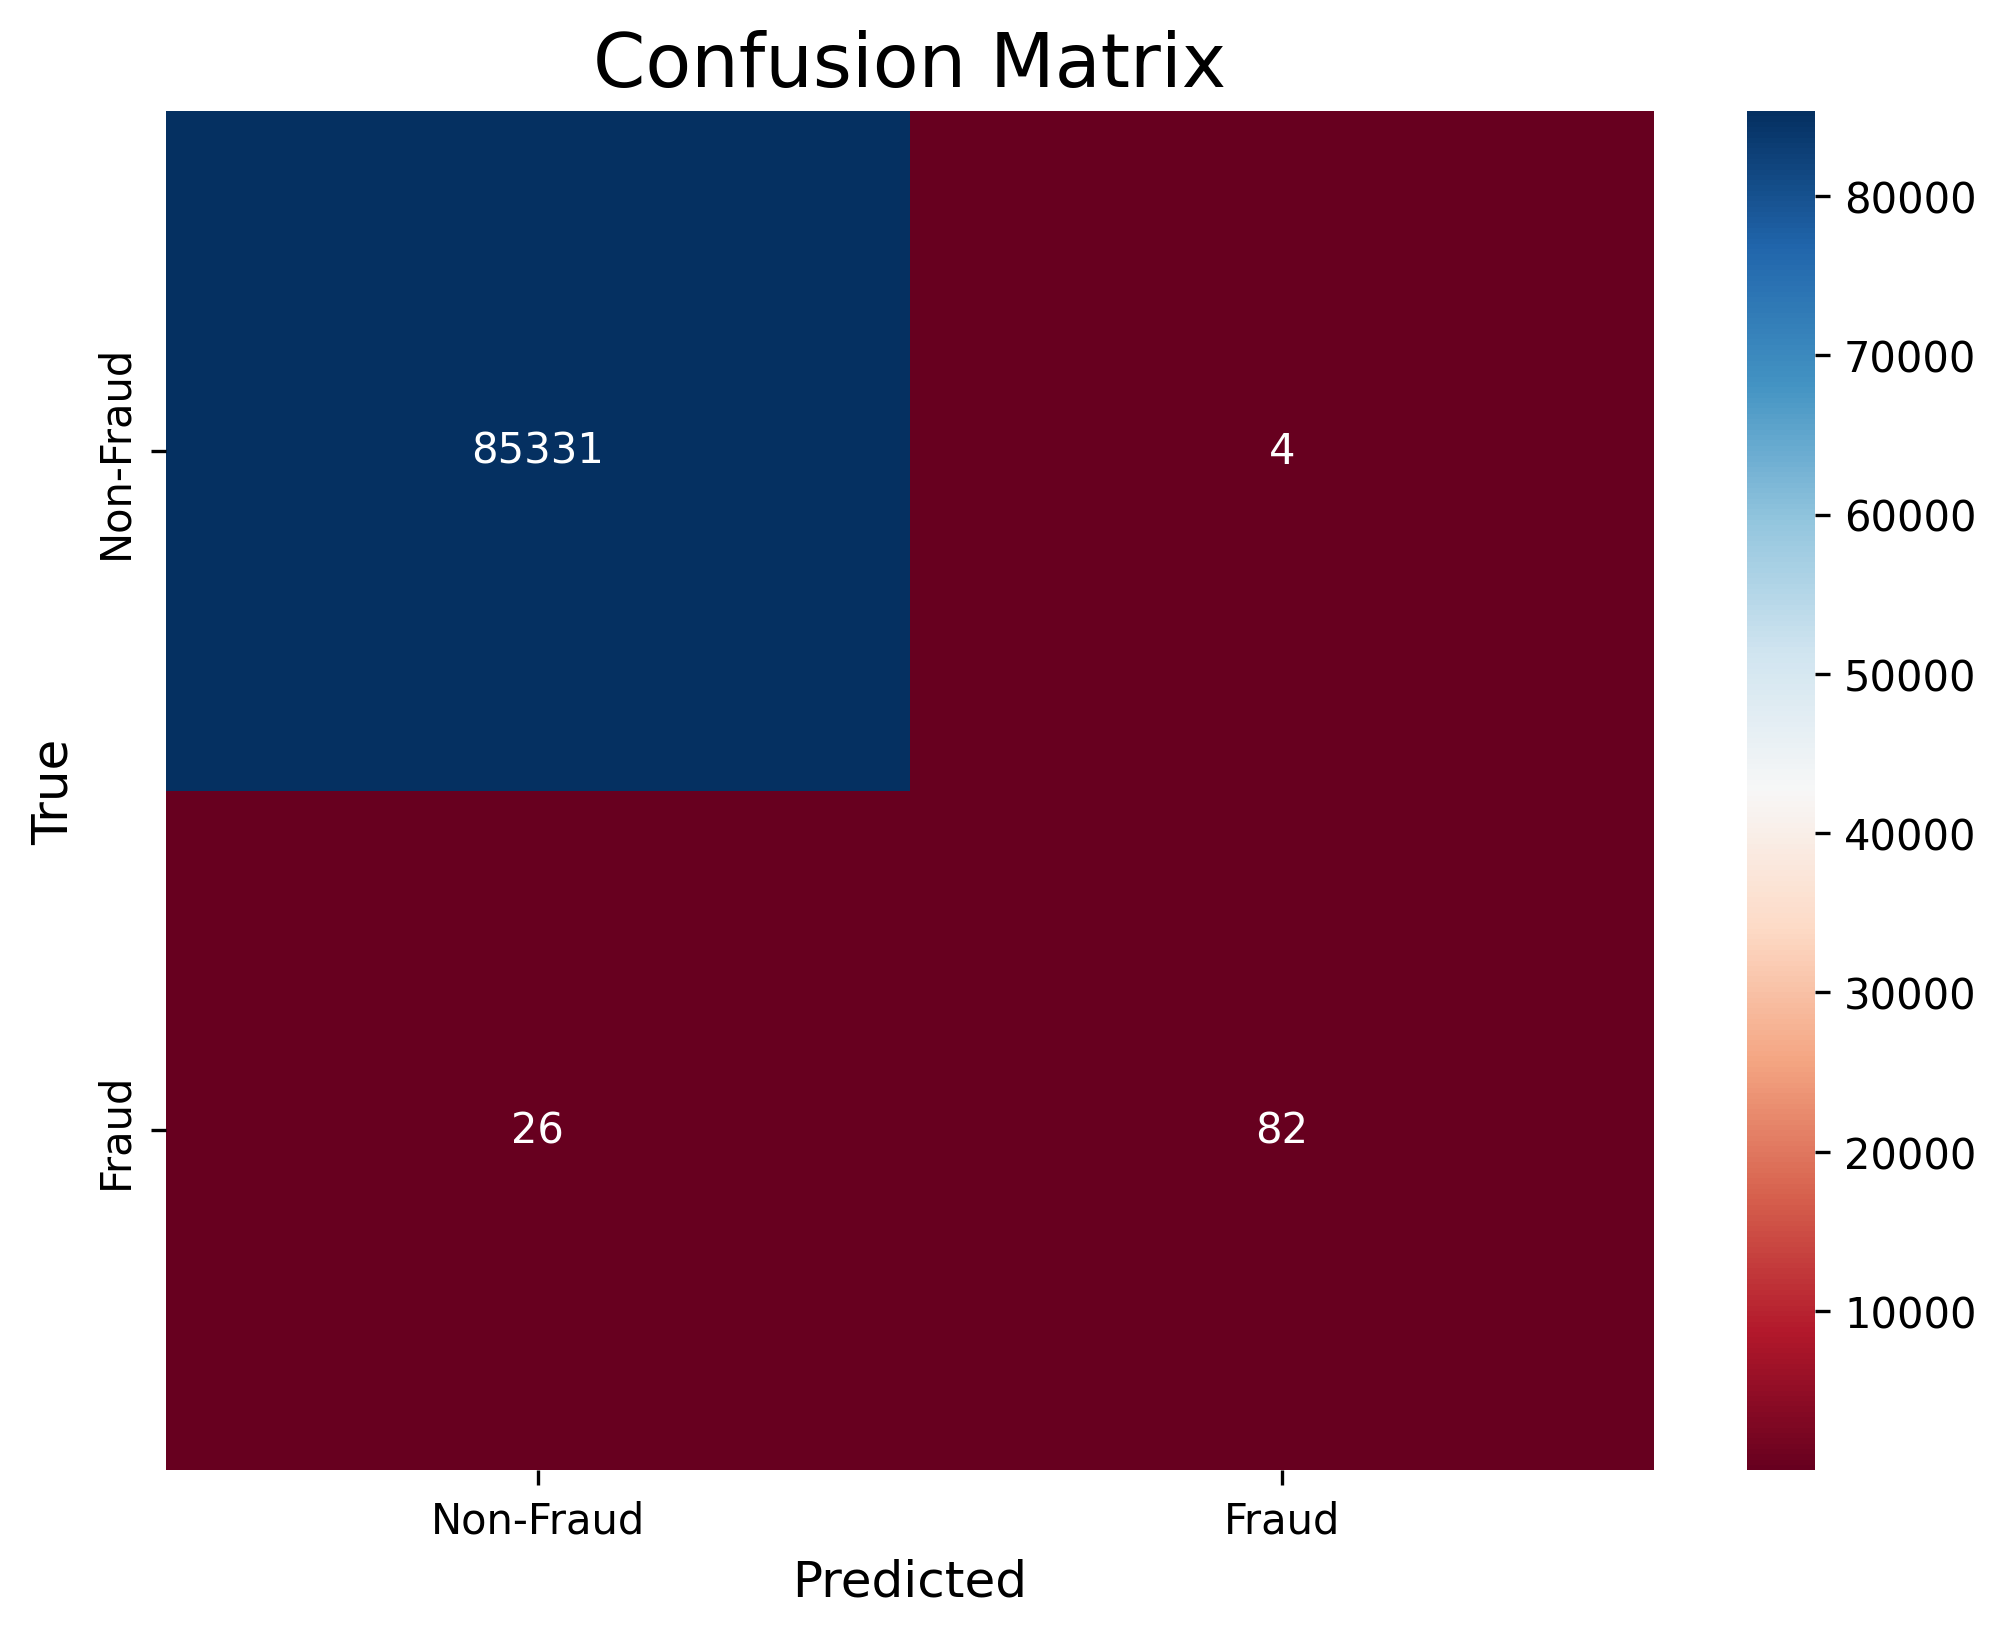
\includegraphics[width=1.0\textwidth]{images/confusion_matrix_randomforest.png}
        \caption{Confusion Matrix for Random Forest}
        \label{fig:confusion_matrix_rf}
    \end{minipage}\hfill
    \begin{minipage}{0.49\textwidth}
        \centering
        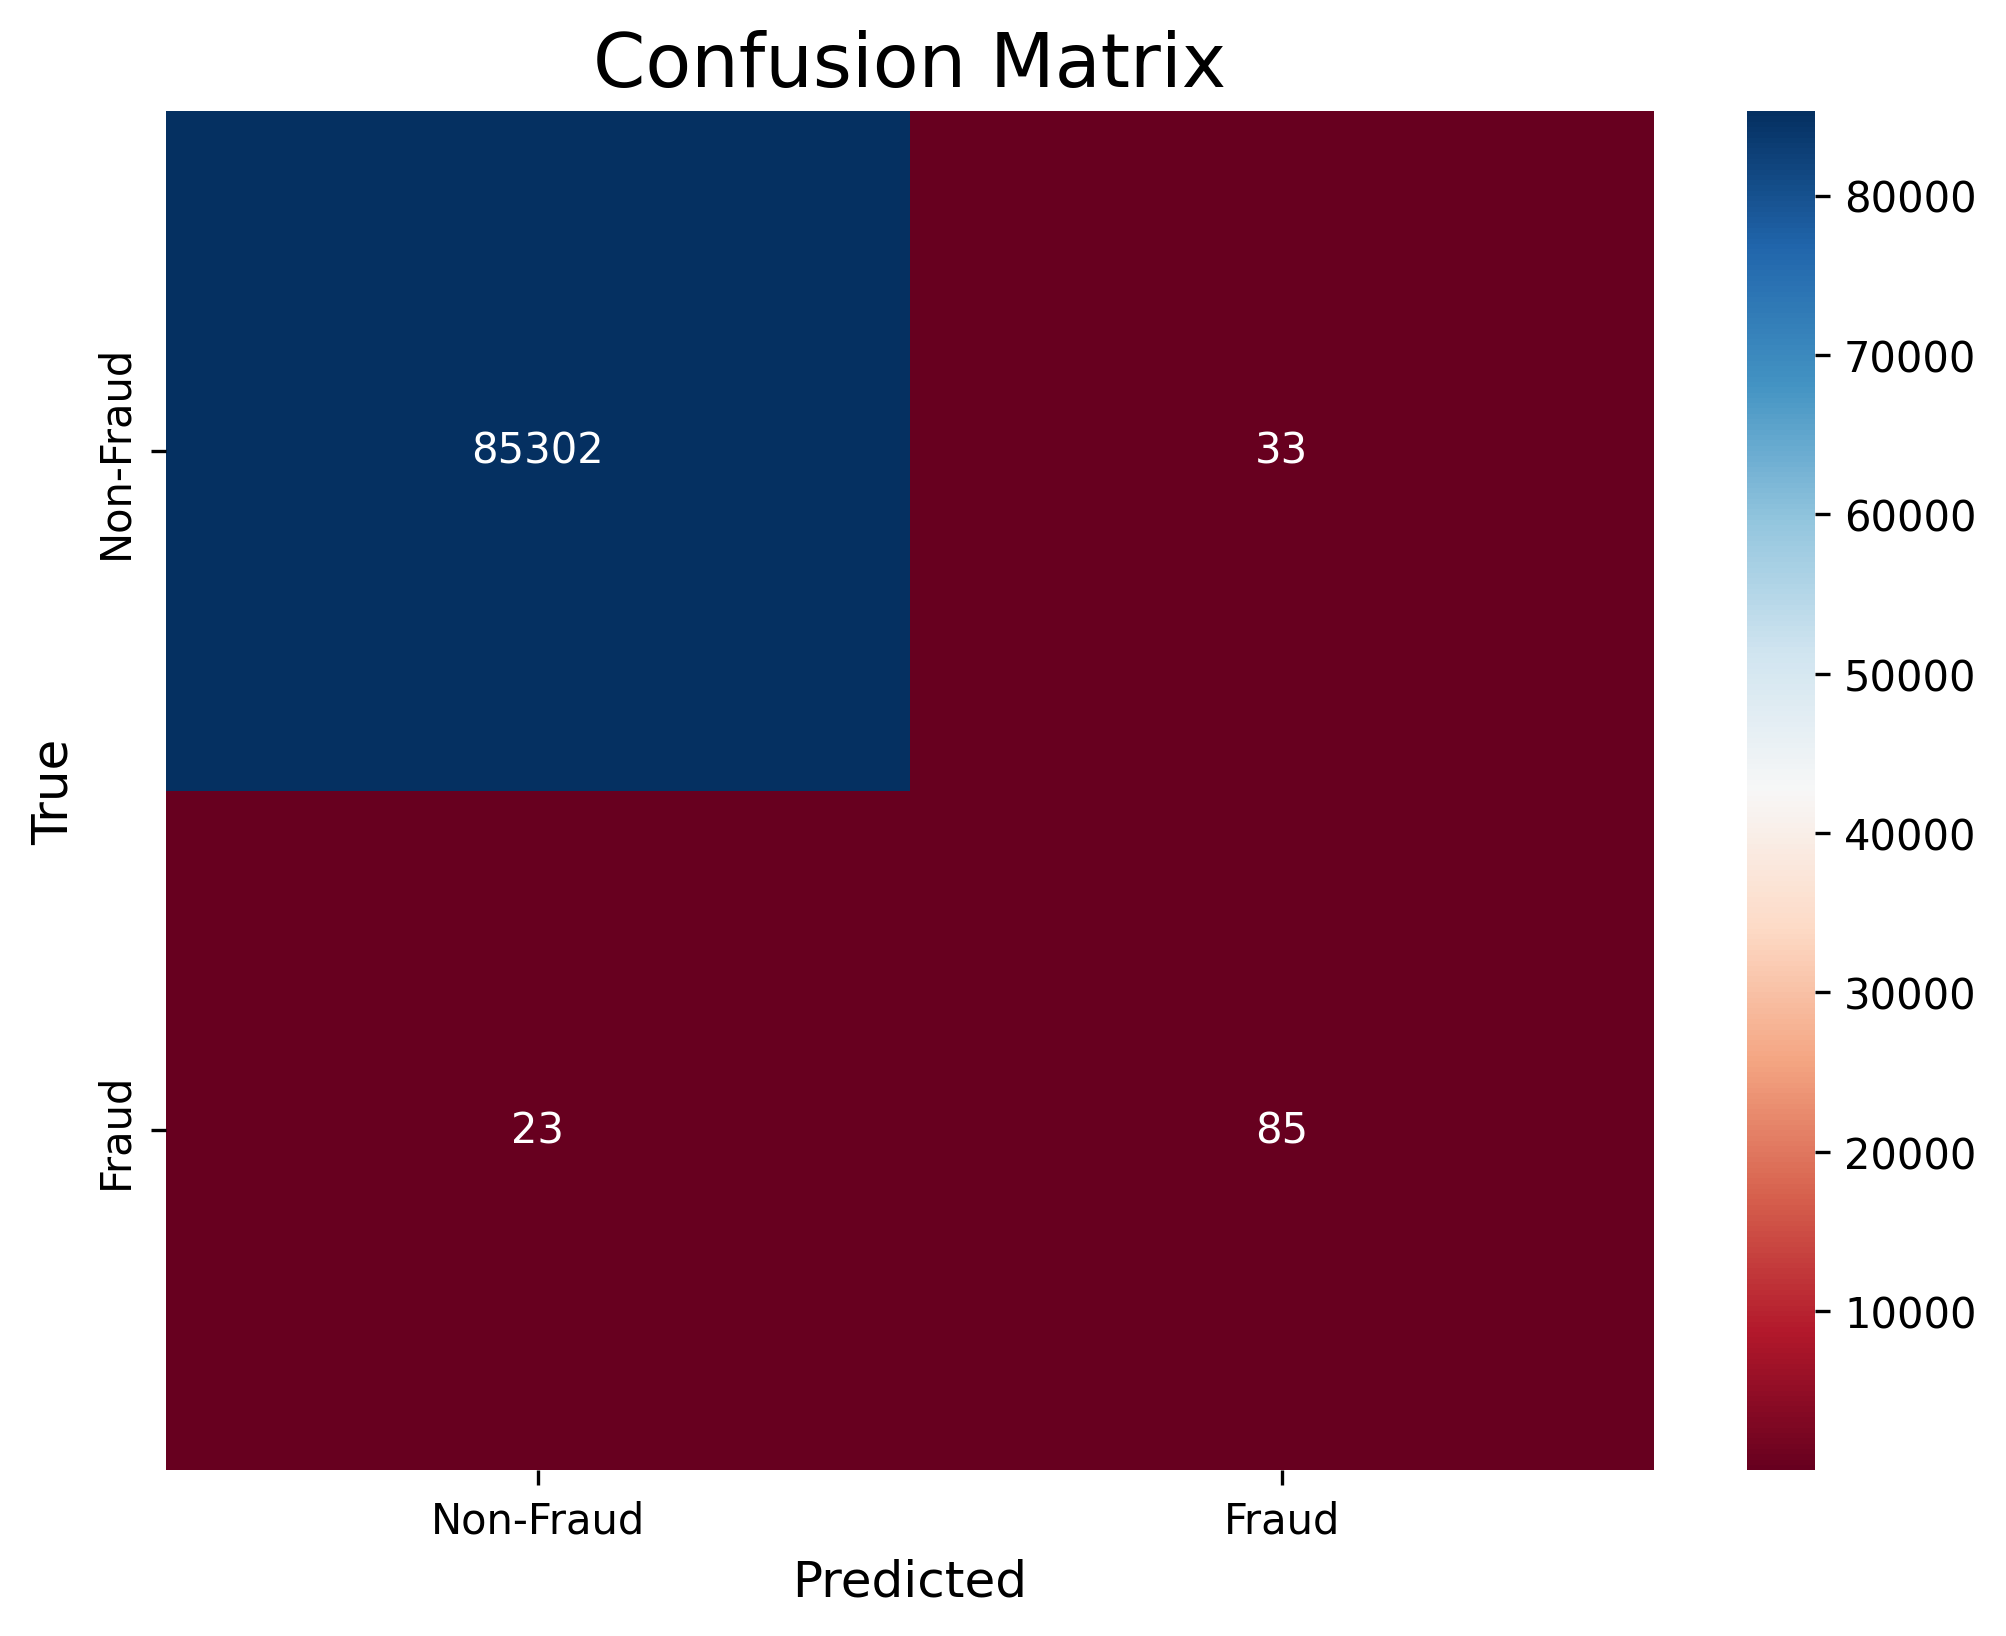
\includegraphics[width=1.0\textwidth]{images/confusion_matrix_mlp.png}
        \caption{Confusion Matrix for Multi-Layer Perceptron}
        \label{fig:confusion_matrix_mlp}
    \end{minipage}
\end{figure}

\begin{figure}[H]
    \centering
    \begin{minipage}{0.49\textwidth}
        \centering
        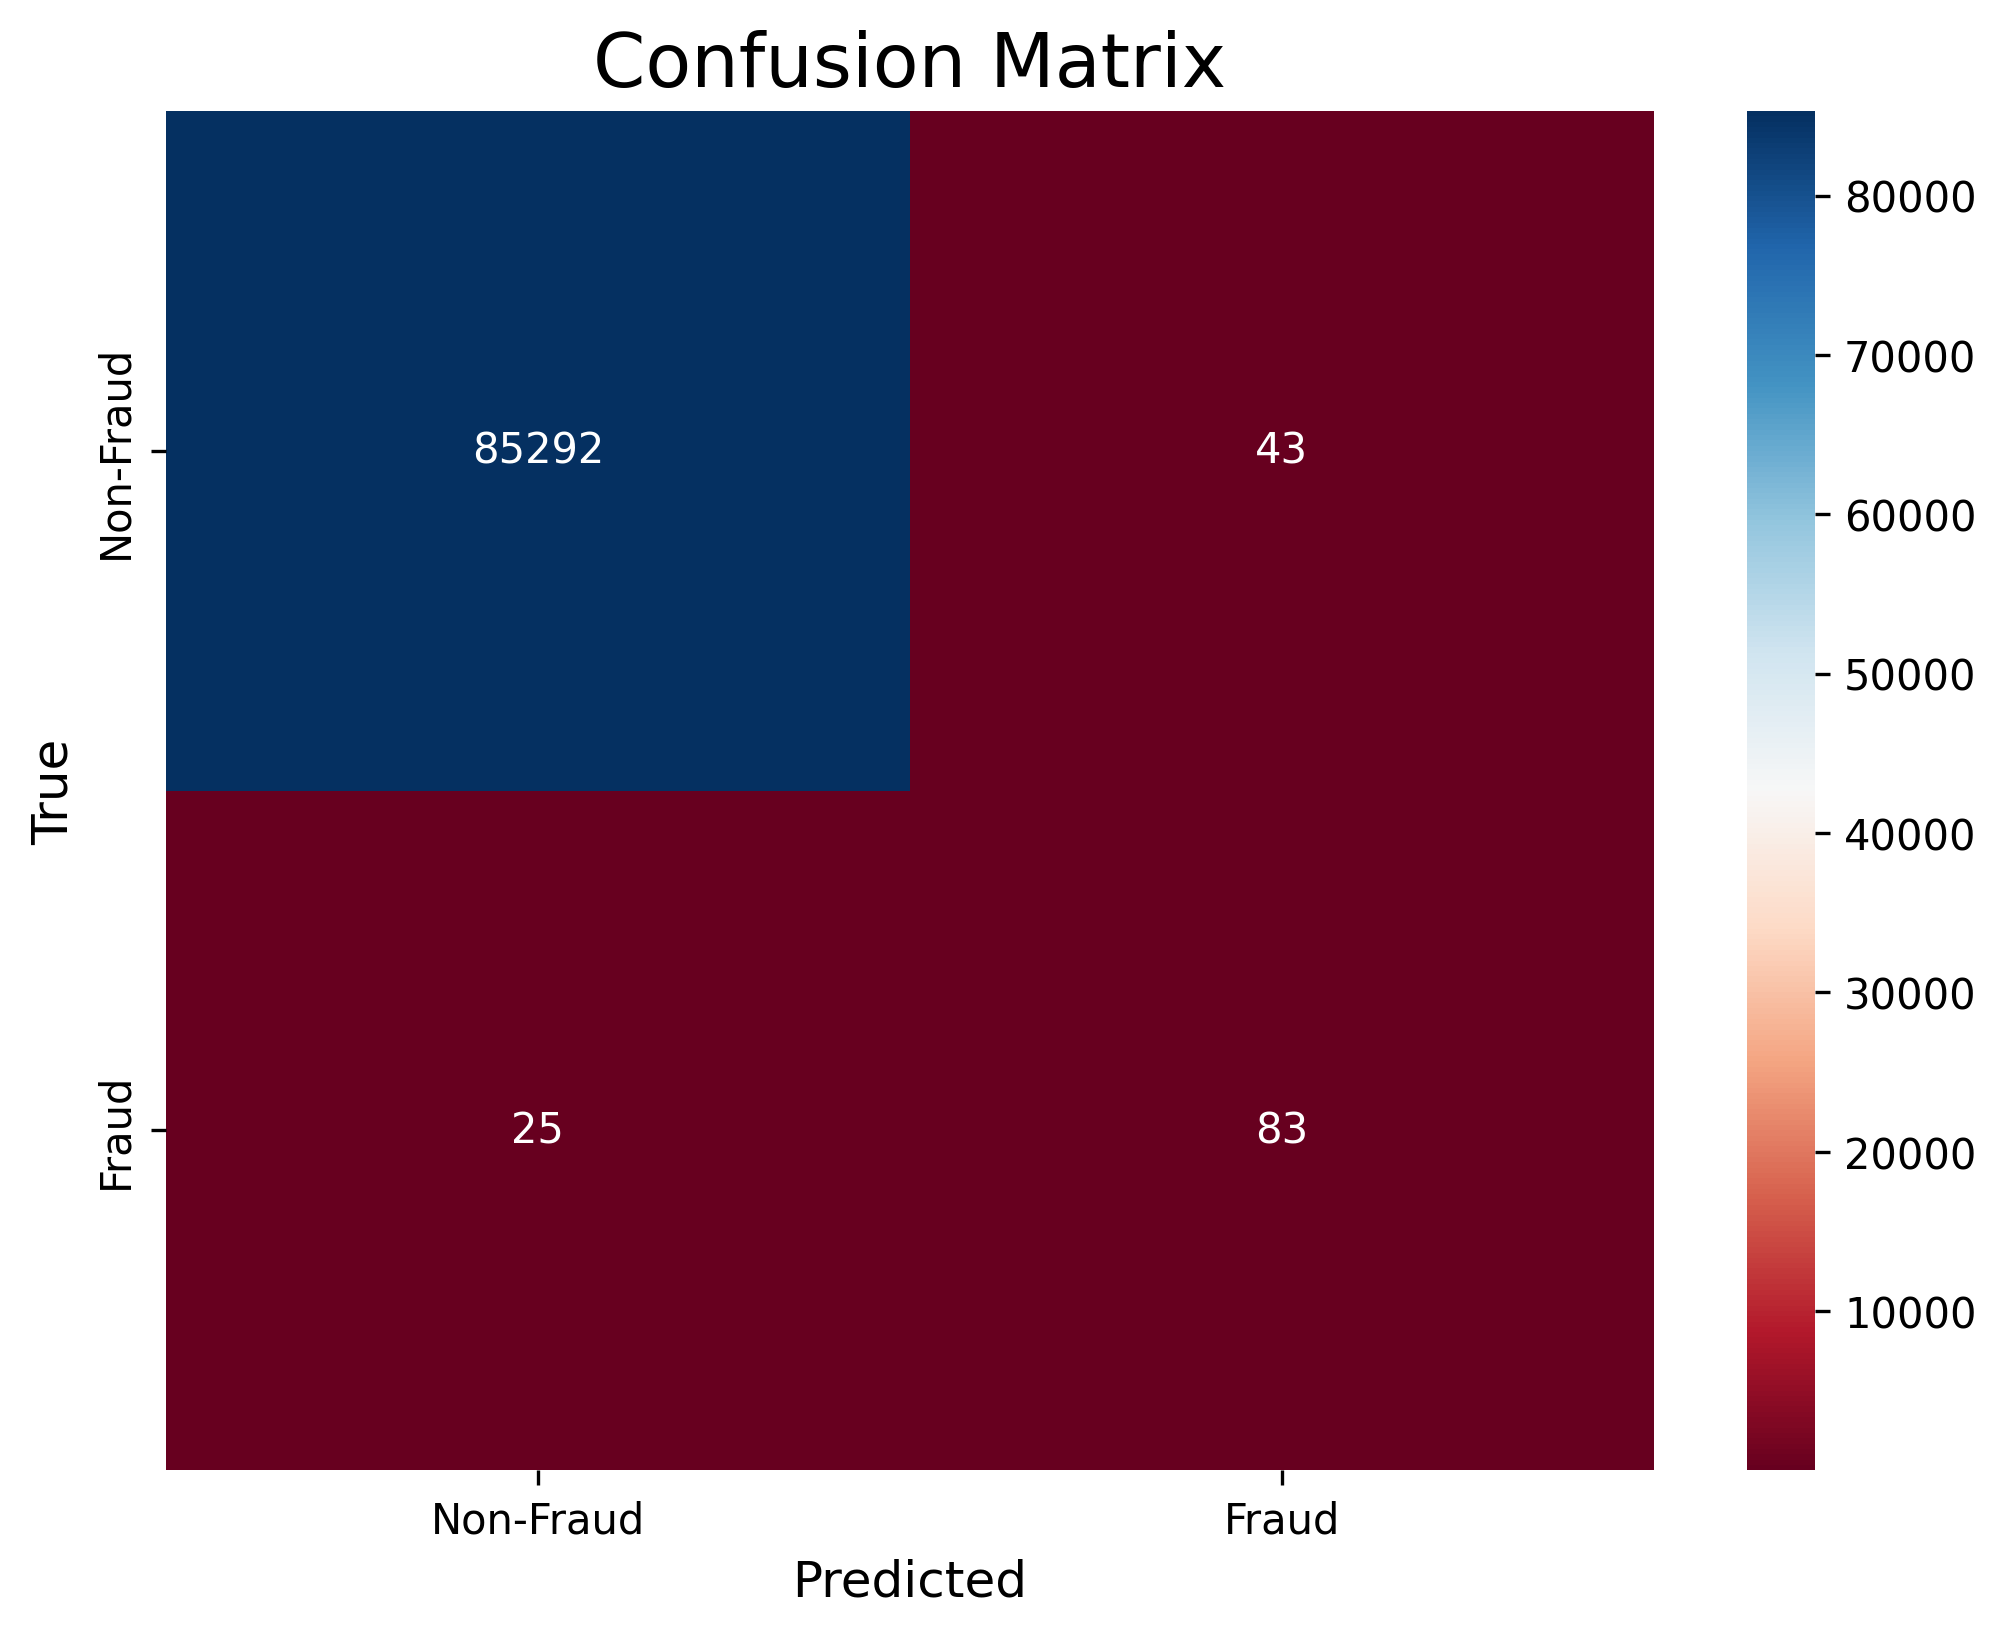
\includegraphics[width=1.0\textwidth]{images/confusion_matrix_lstm.png}
        \caption{Confusion Matrix for LSTM}
        \label{fig:confusion_matrix_lstm}
    \end{minipage}\hfill
    \begin{minipage}{0.49\textwidth}
        \centering
        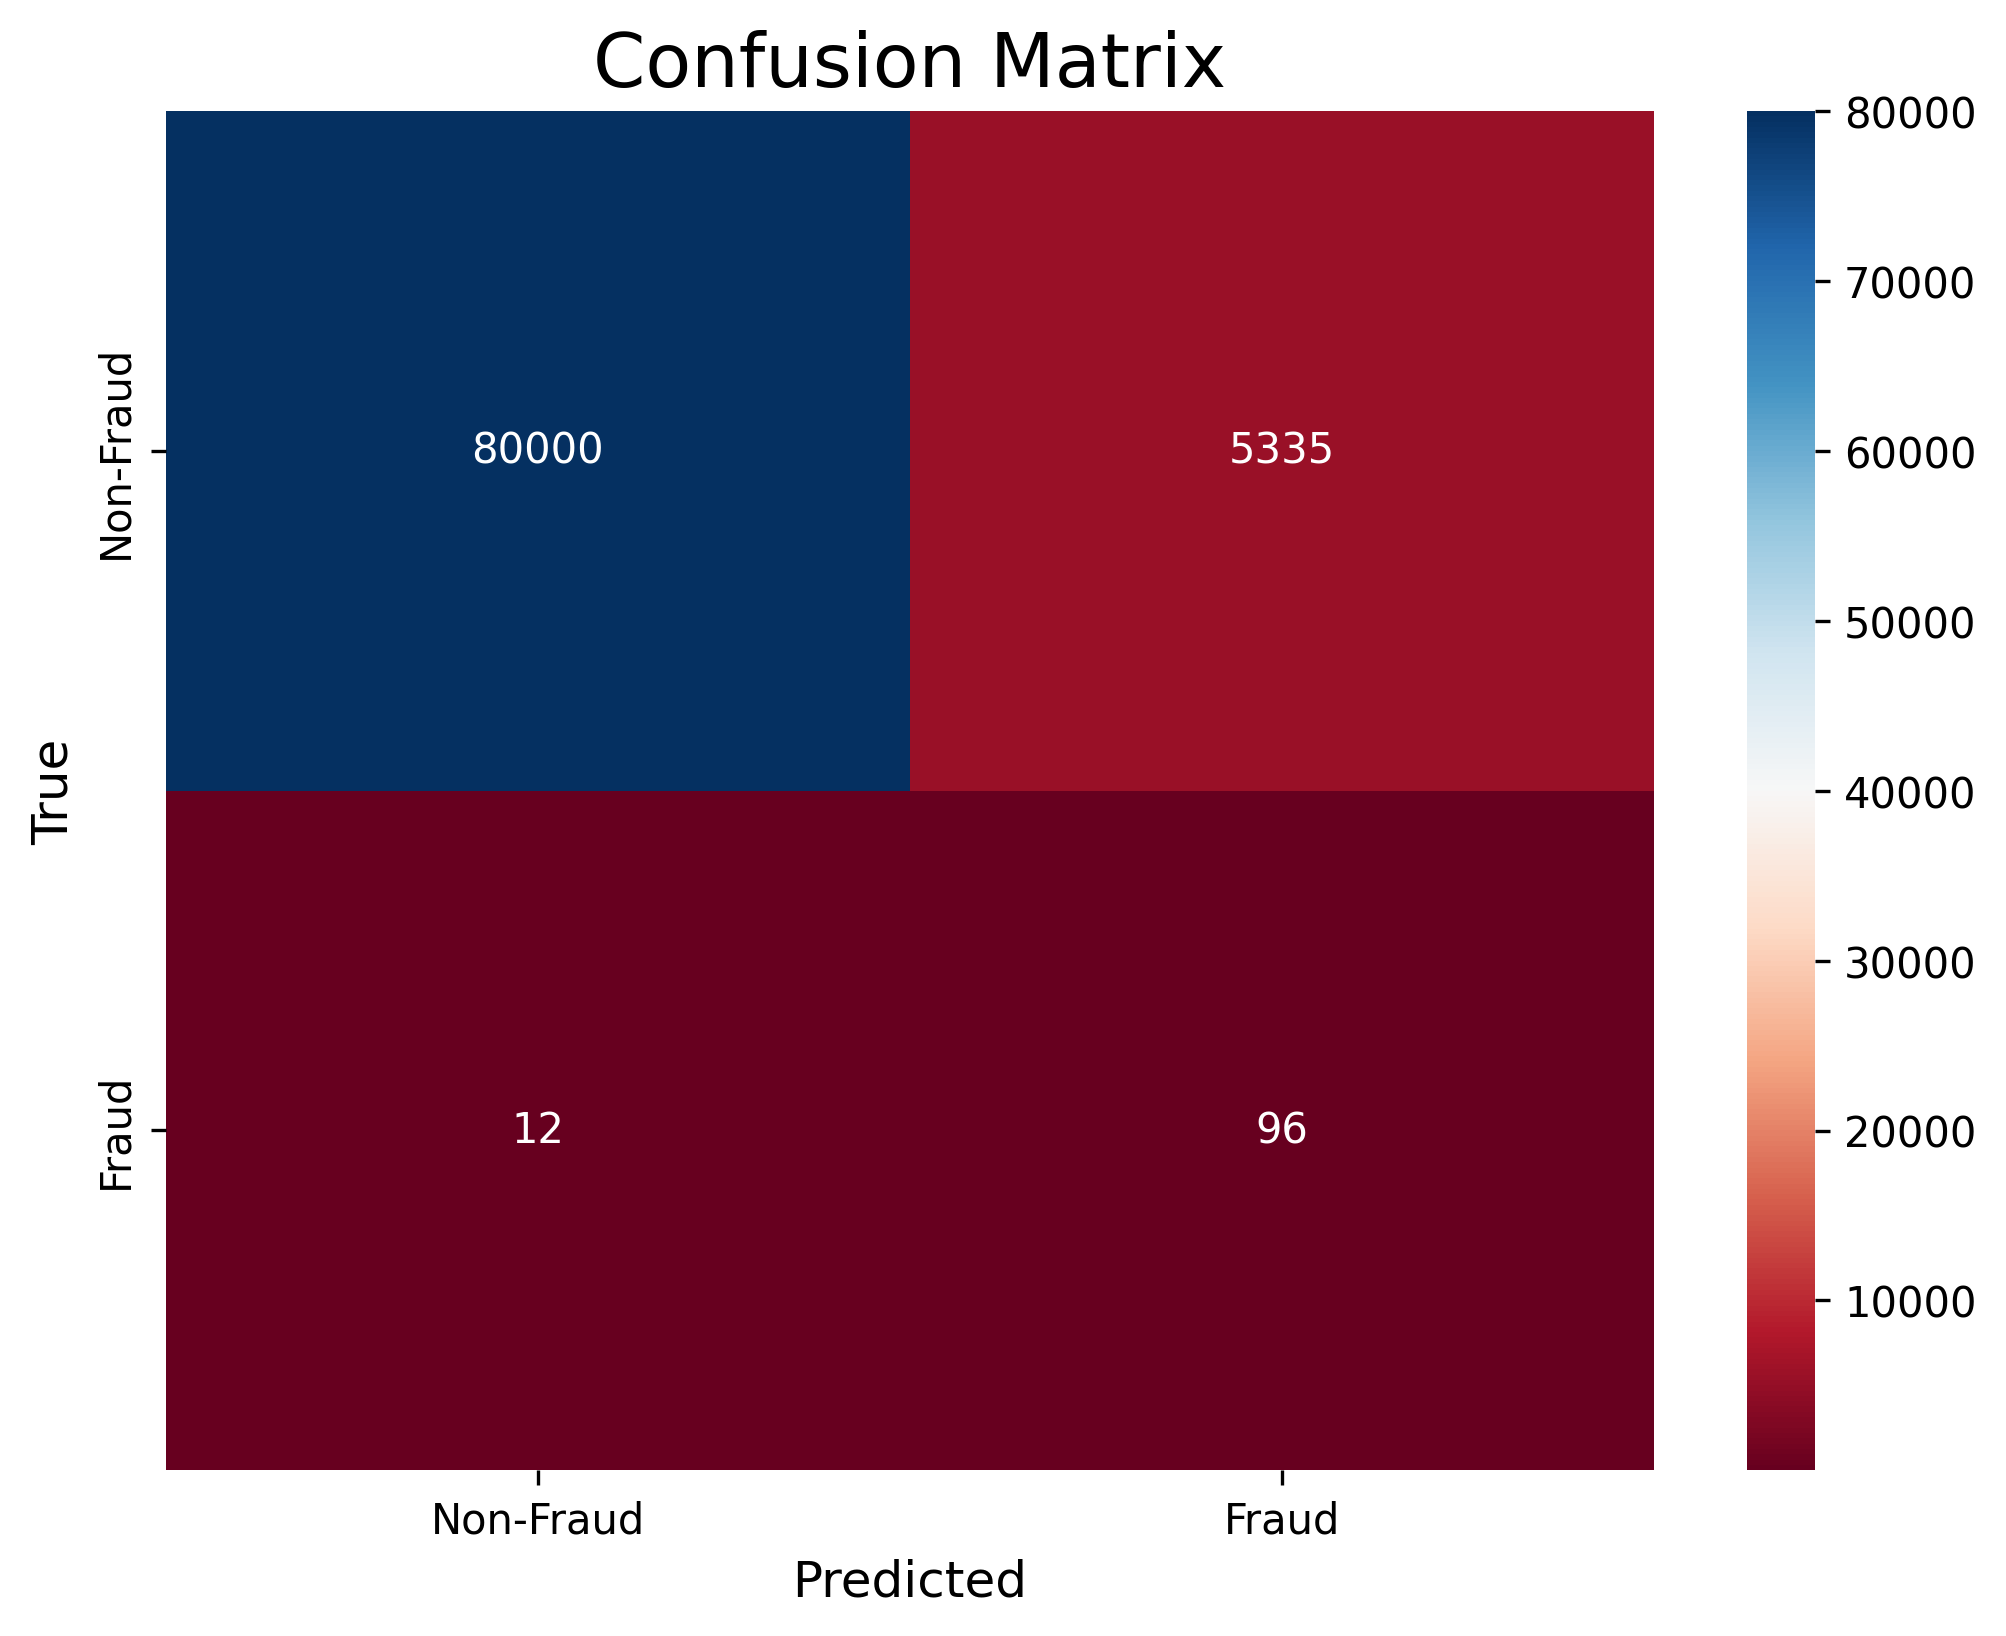
\includegraphics[width=1.0\textwidth]{images/confusion_matrix_transformer.png}
        \caption{Confusion Matrix for Transformer}
        \label{fig:confusion_matrix_transformer}
    \end{minipage}
\end{figure}

As seen in Table~\ref{tab:model_performance_bce}, the Transformer model achieves a fraud-class recall (0.89) that closely approaches that of Logistic Regression (0.90), and surpasses the other models (Random Forest, MLP, LSTM) in capturing the minority class. This suggests that the Transformer’s self-attention mechanism is effective at identifying subtle patterns indicative of fraud. However, its non-fraud recall (0.94) is slightly lower than that of the models relying on simpler decision boundaries or ensemble/tree-based methods, which all achieve near-perfect recall on non-fraud cases.

This disparity may indicate that the Transformer, in striving to improve detection of the minority class, makes trade-offs that reduce its ability to consistently classify the majority class. Put another way, the Transformer might be more willing to flag borderline cases as potentially fraudulent, thereby catching more actual frauds but occasionally misclassifying some legitimate transactions. Such a balance, while potentially beneficial from a risk management perspective, may still be optimized further.

\subsection{Impact of Focal Loss and Varying \(\gamma\)}

To delve deeper into refining the Transformer's performance—particularly to better handle imbalanced data and further improve its minority-class recall without substantially harming its majority-class performance—we next explore the application of Focal Loss with varying \(\gamma\) values (0.5, 1, 2, 3, 4, 5). By adjusting \(\gamma\), we aim to shift the model’s focus more intelligently onto hard-to-classify fraud cases, potentially unlocking a better balance between correctly identifying rare instances of fraud and maintaining robust performance on non-fraud transactions.

As shown in Table~\ref{tab:focal_gamma} and the corresponding confusion matrices, varying \(\gamma\) in the Focal Loss significantly influences the Transformer's performance trade-offs between fraud and non-fraud recall. Lower \(\gamma\) values (e.g., 0.5) lead the Transformer to focus more aggressively on the hardest positive cases, improving fraud recall at the cost of a notable decline in non-fraud recall. Conversely, certain higher \(\gamma\) values (e.g., 1 or 3) can restore stronger performance on the majority class but slightly reduce fraud-class sensitivity. 

\begin{table}[h]
\centering
\caption{Transformer Performance Under Focal Loss with Varying \(\gamma\)}
\label{tab:focal_gamma}
\begin{tabular}{lccc}
\hline
\(\gamma\) & Recall (Non-Fraud) & Recall (Fraud) & ROC AUC Score \\
\hline
0.5 & 0.851 & 0.935 & 0.893 \\
1   & 0.951 & 0.880 & 0.915 \\
2   & 0.931 & 0.917 & 0.924 \\
3   & 0.971 & 0.880 & 0.925 \\
4   & 0.950 & 0.889 & 0.920 \\
5   & 0.898 & 0.926 & 0.912 \\
\hline
\end{tabular}
\end{table}

\begin{figure}[H]
    \centering
    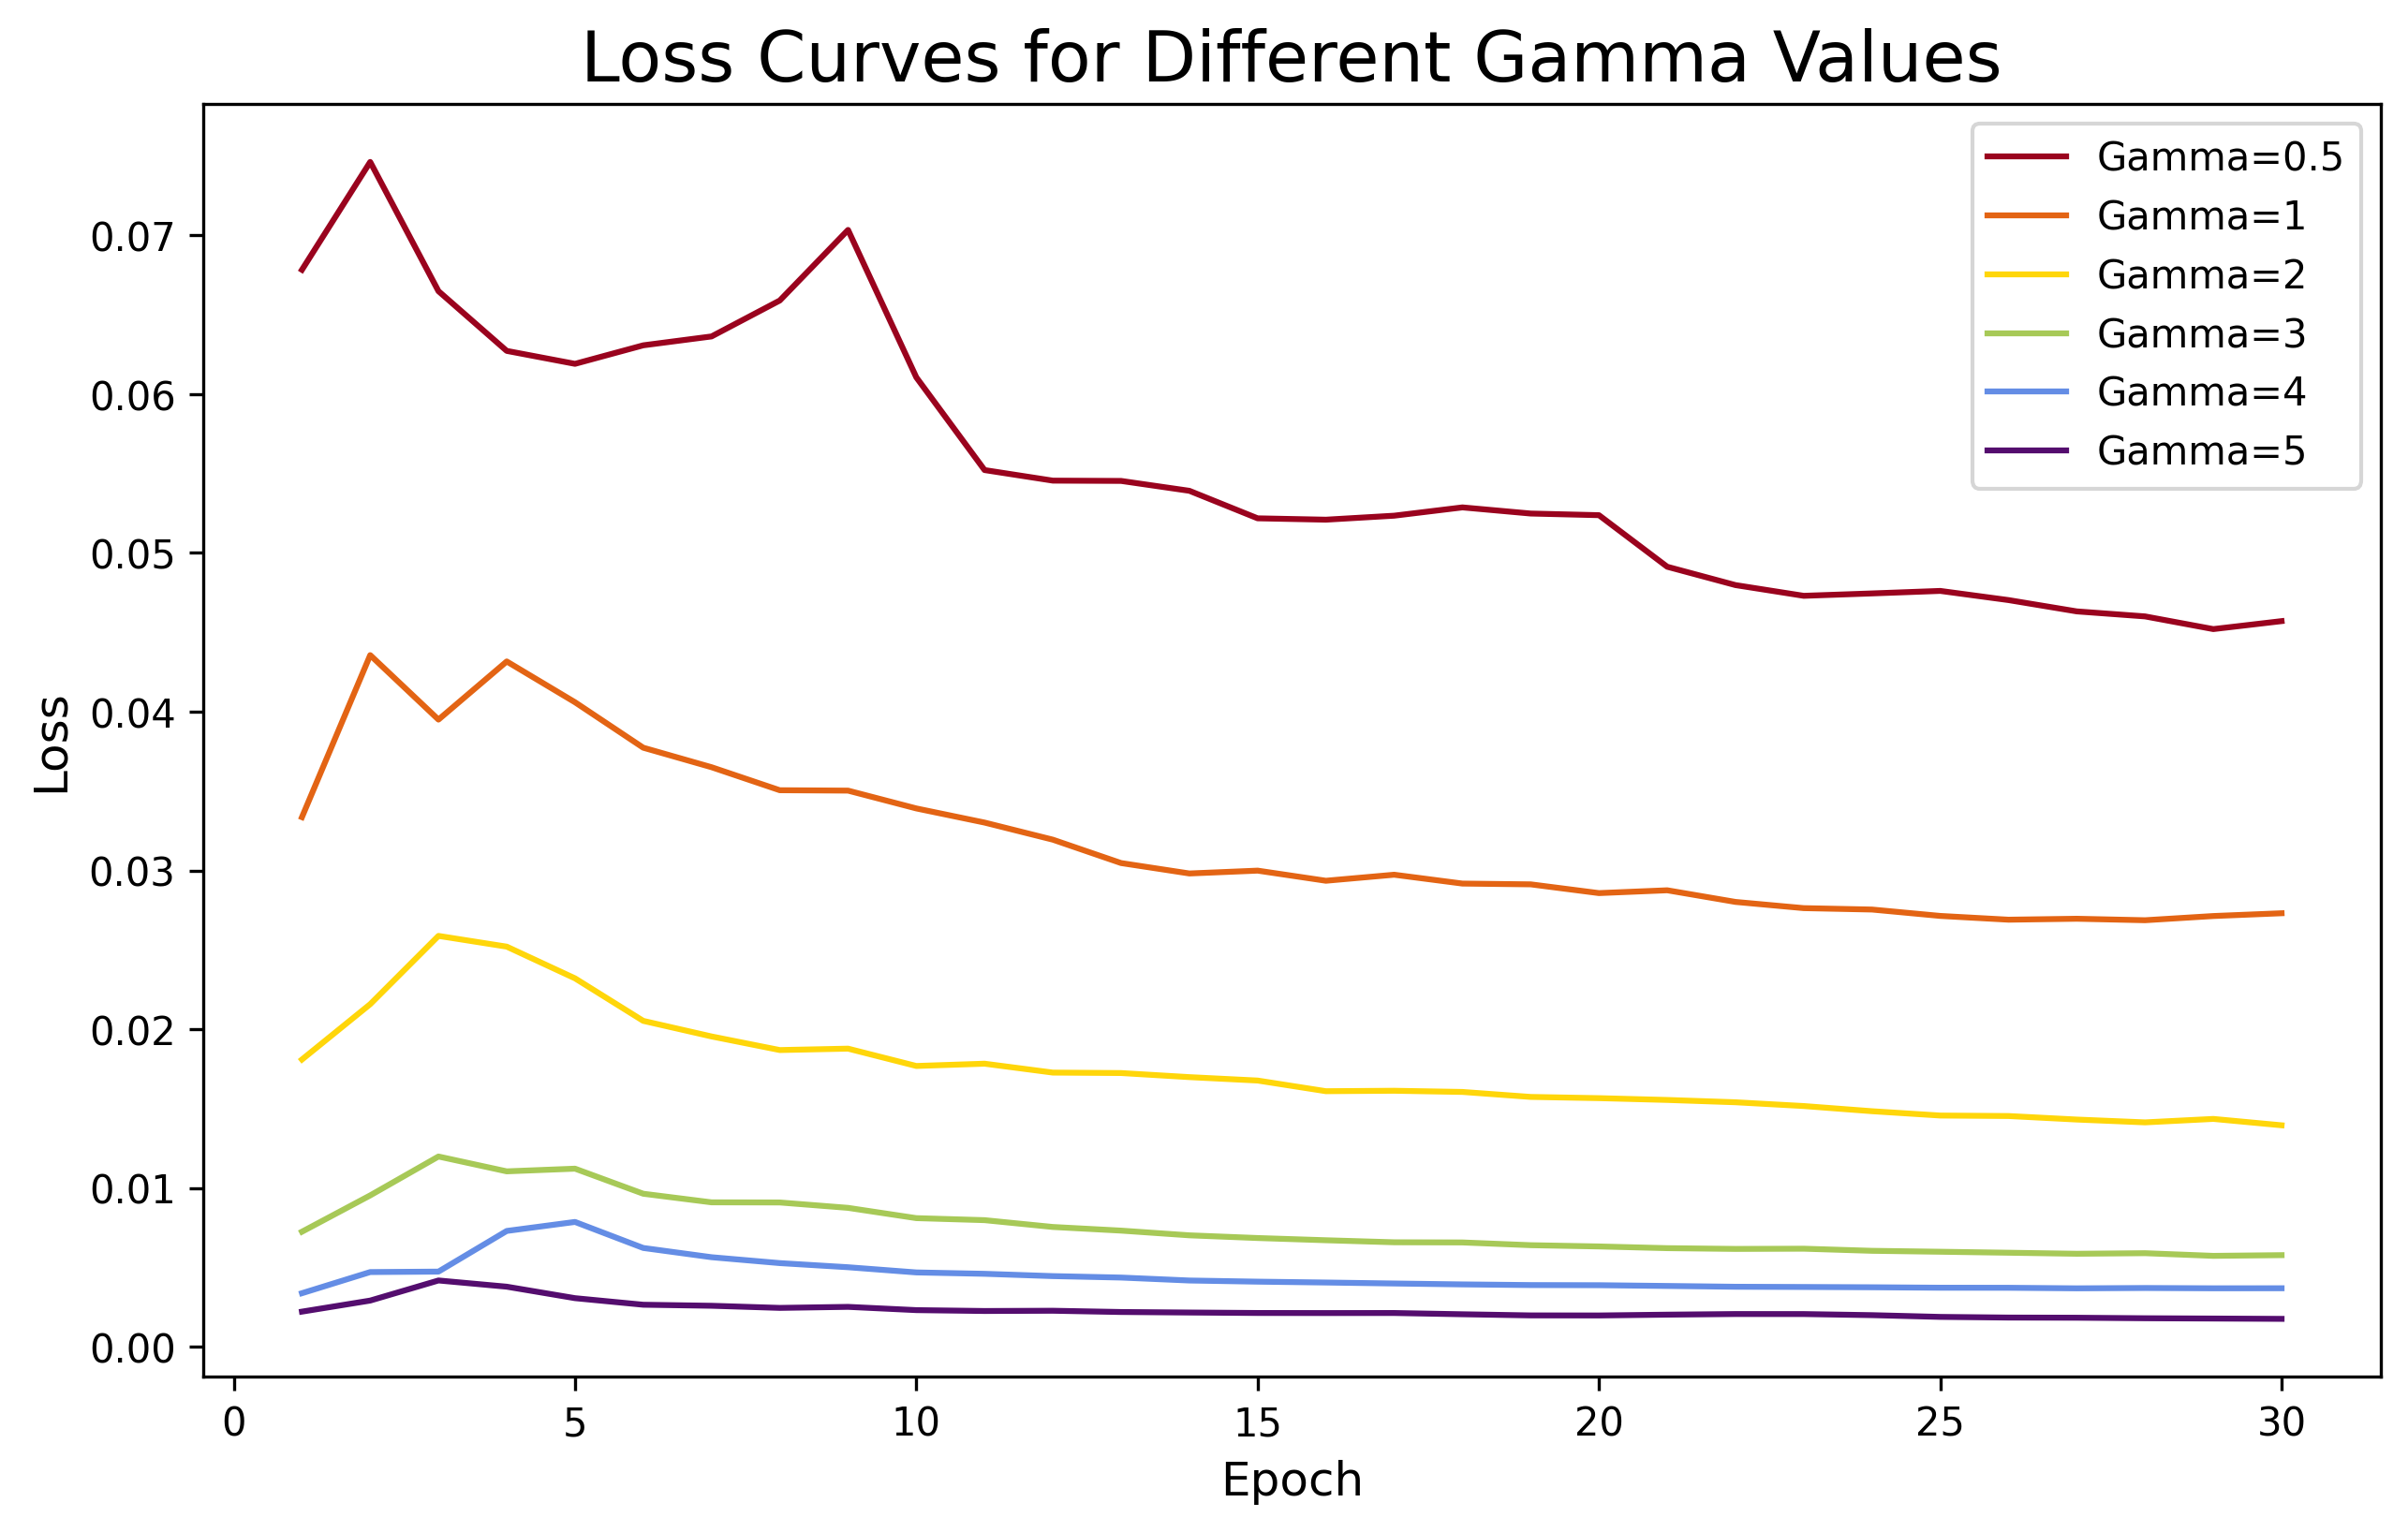
\includegraphics[width=0.65\textwidth]{images/loss_curves_transformer.png}
    \caption{Loss Curves of Transformer For Different Gammas}
    \label{fig:loss_curves_transformer}
\end{figure}

Figures~\ref{fig:confusion_matrix_transformer_0.5} through \ref{fig:confusion_matrix_transformer_5} present the corresponding confusion matrices for each \(\gamma\) value. Among these configurations, \(\gamma = 2\) stands out as particularly promising. This value is higher than its performance at other values, with the sole exception of the case when \(\gamma = 0.5\). Moreover, it outperforms the fraud recall of Logistic Regression. At the same time, its non-fraud recall (0.931) remains relatively high, indicating that the model has not overly sacrificed performance on the majority class. The ROC AUC score (0.924) further confirms the balanced improvements achieved by \(\gamma = 2\).

\begin{figure}[H]
    \centering
    \begin{minipage}{0.49\textwidth}
        \centering
        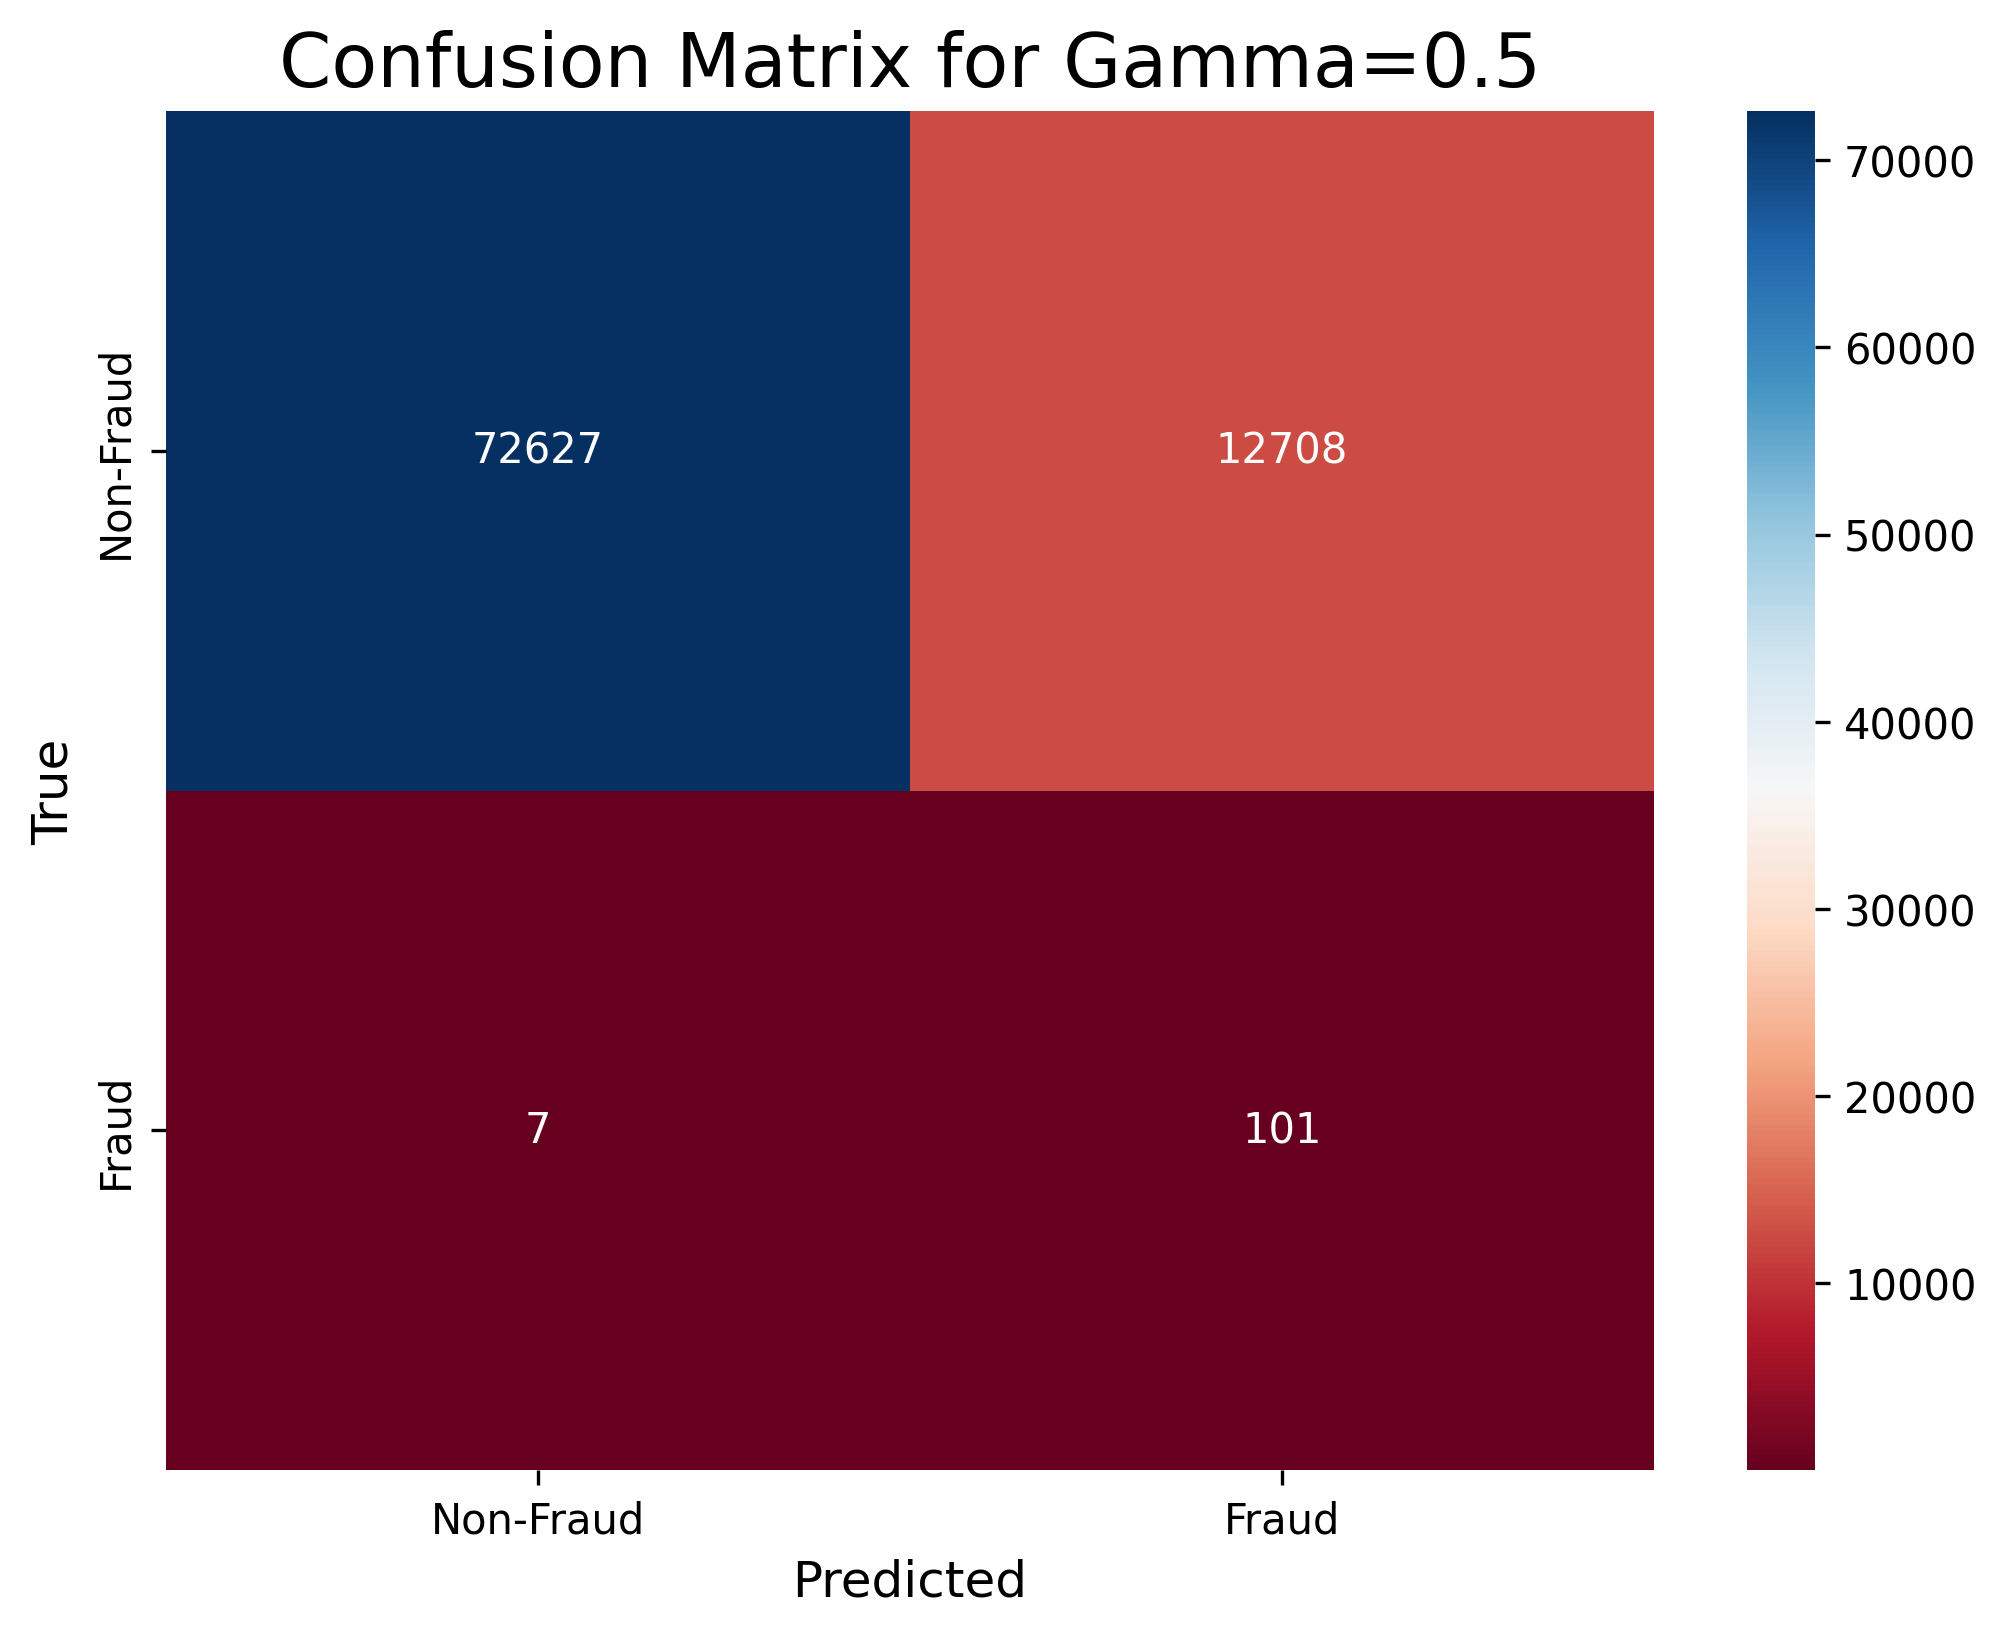
\includegraphics[width=1.0\textwidth]{images/confusion_matrix_transformer_0.5.png}
        \caption{Confusion Matrix for Transformer With Gamma = 0.5}
        \label{fig:confusion_matrix_transformer_0.5}
    \end{minipage}\hfill
    \begin{minipage}{0.49\textwidth}
        \centering
        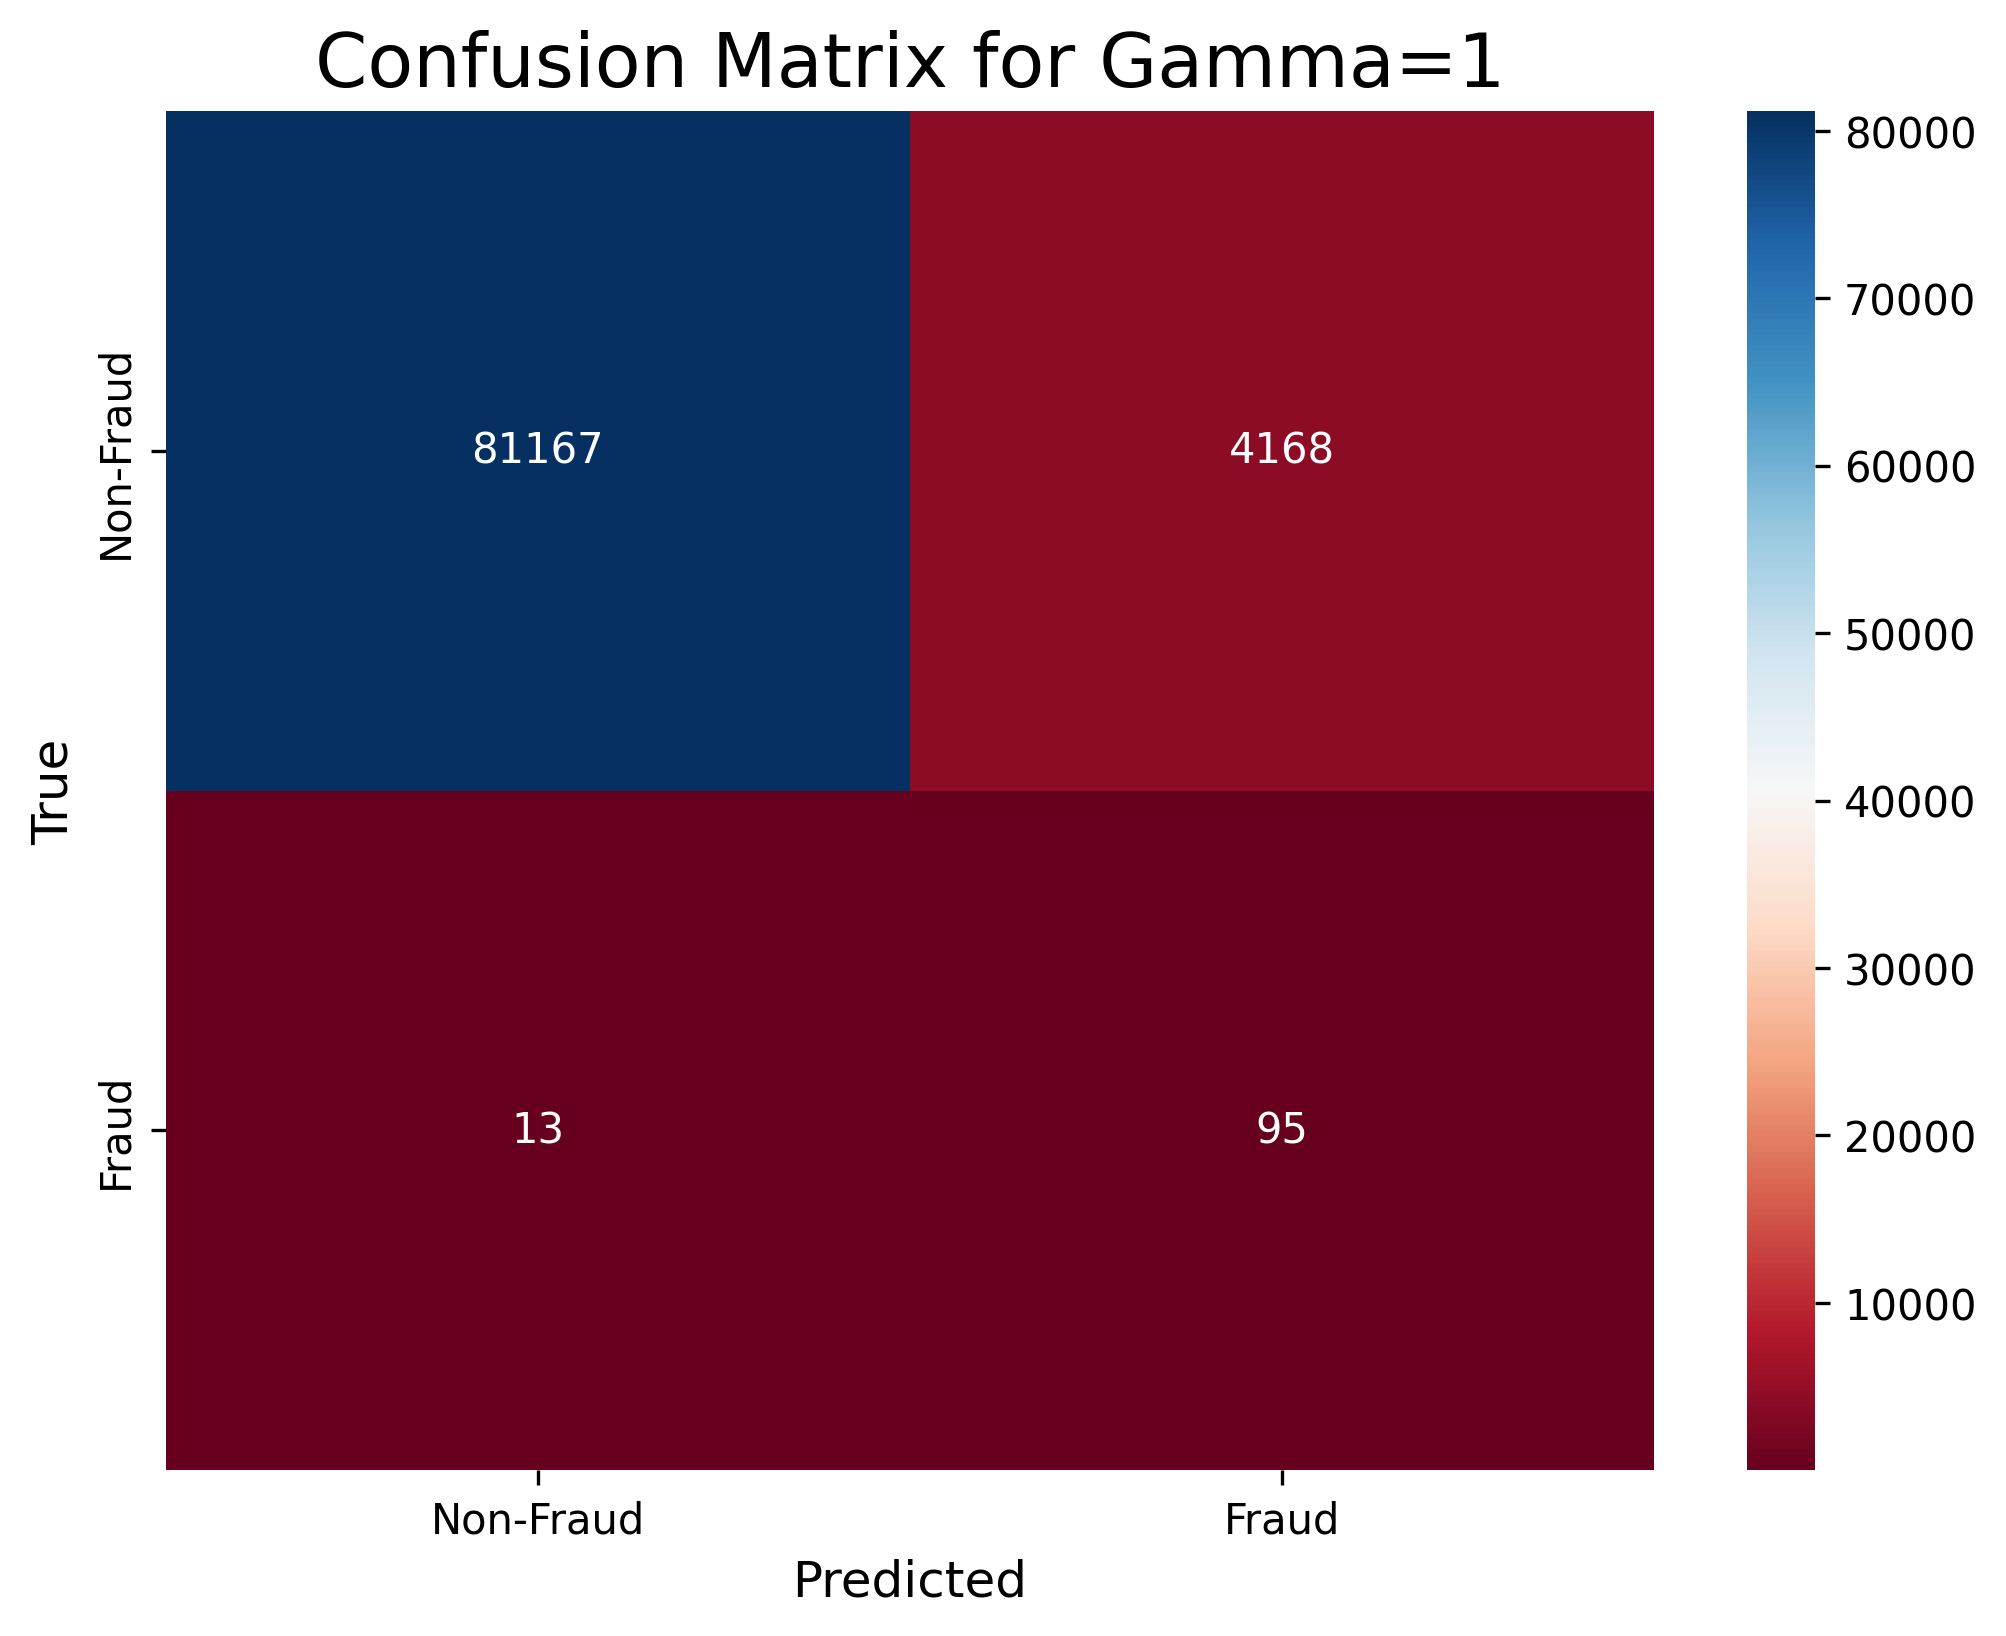
\includegraphics[width=1.0\textwidth]{images/confusion_matrix_transformer_1.png}
        \caption{Confusion Matrix for Transformer With Gamma = 1}
        \label{fig:confusion_matrix_transformer_1}
    \end{minipage}
\end{figure}

\begin{figure}[H]
    \centering
    \begin{minipage}{0.49\textwidth}
        \centering
        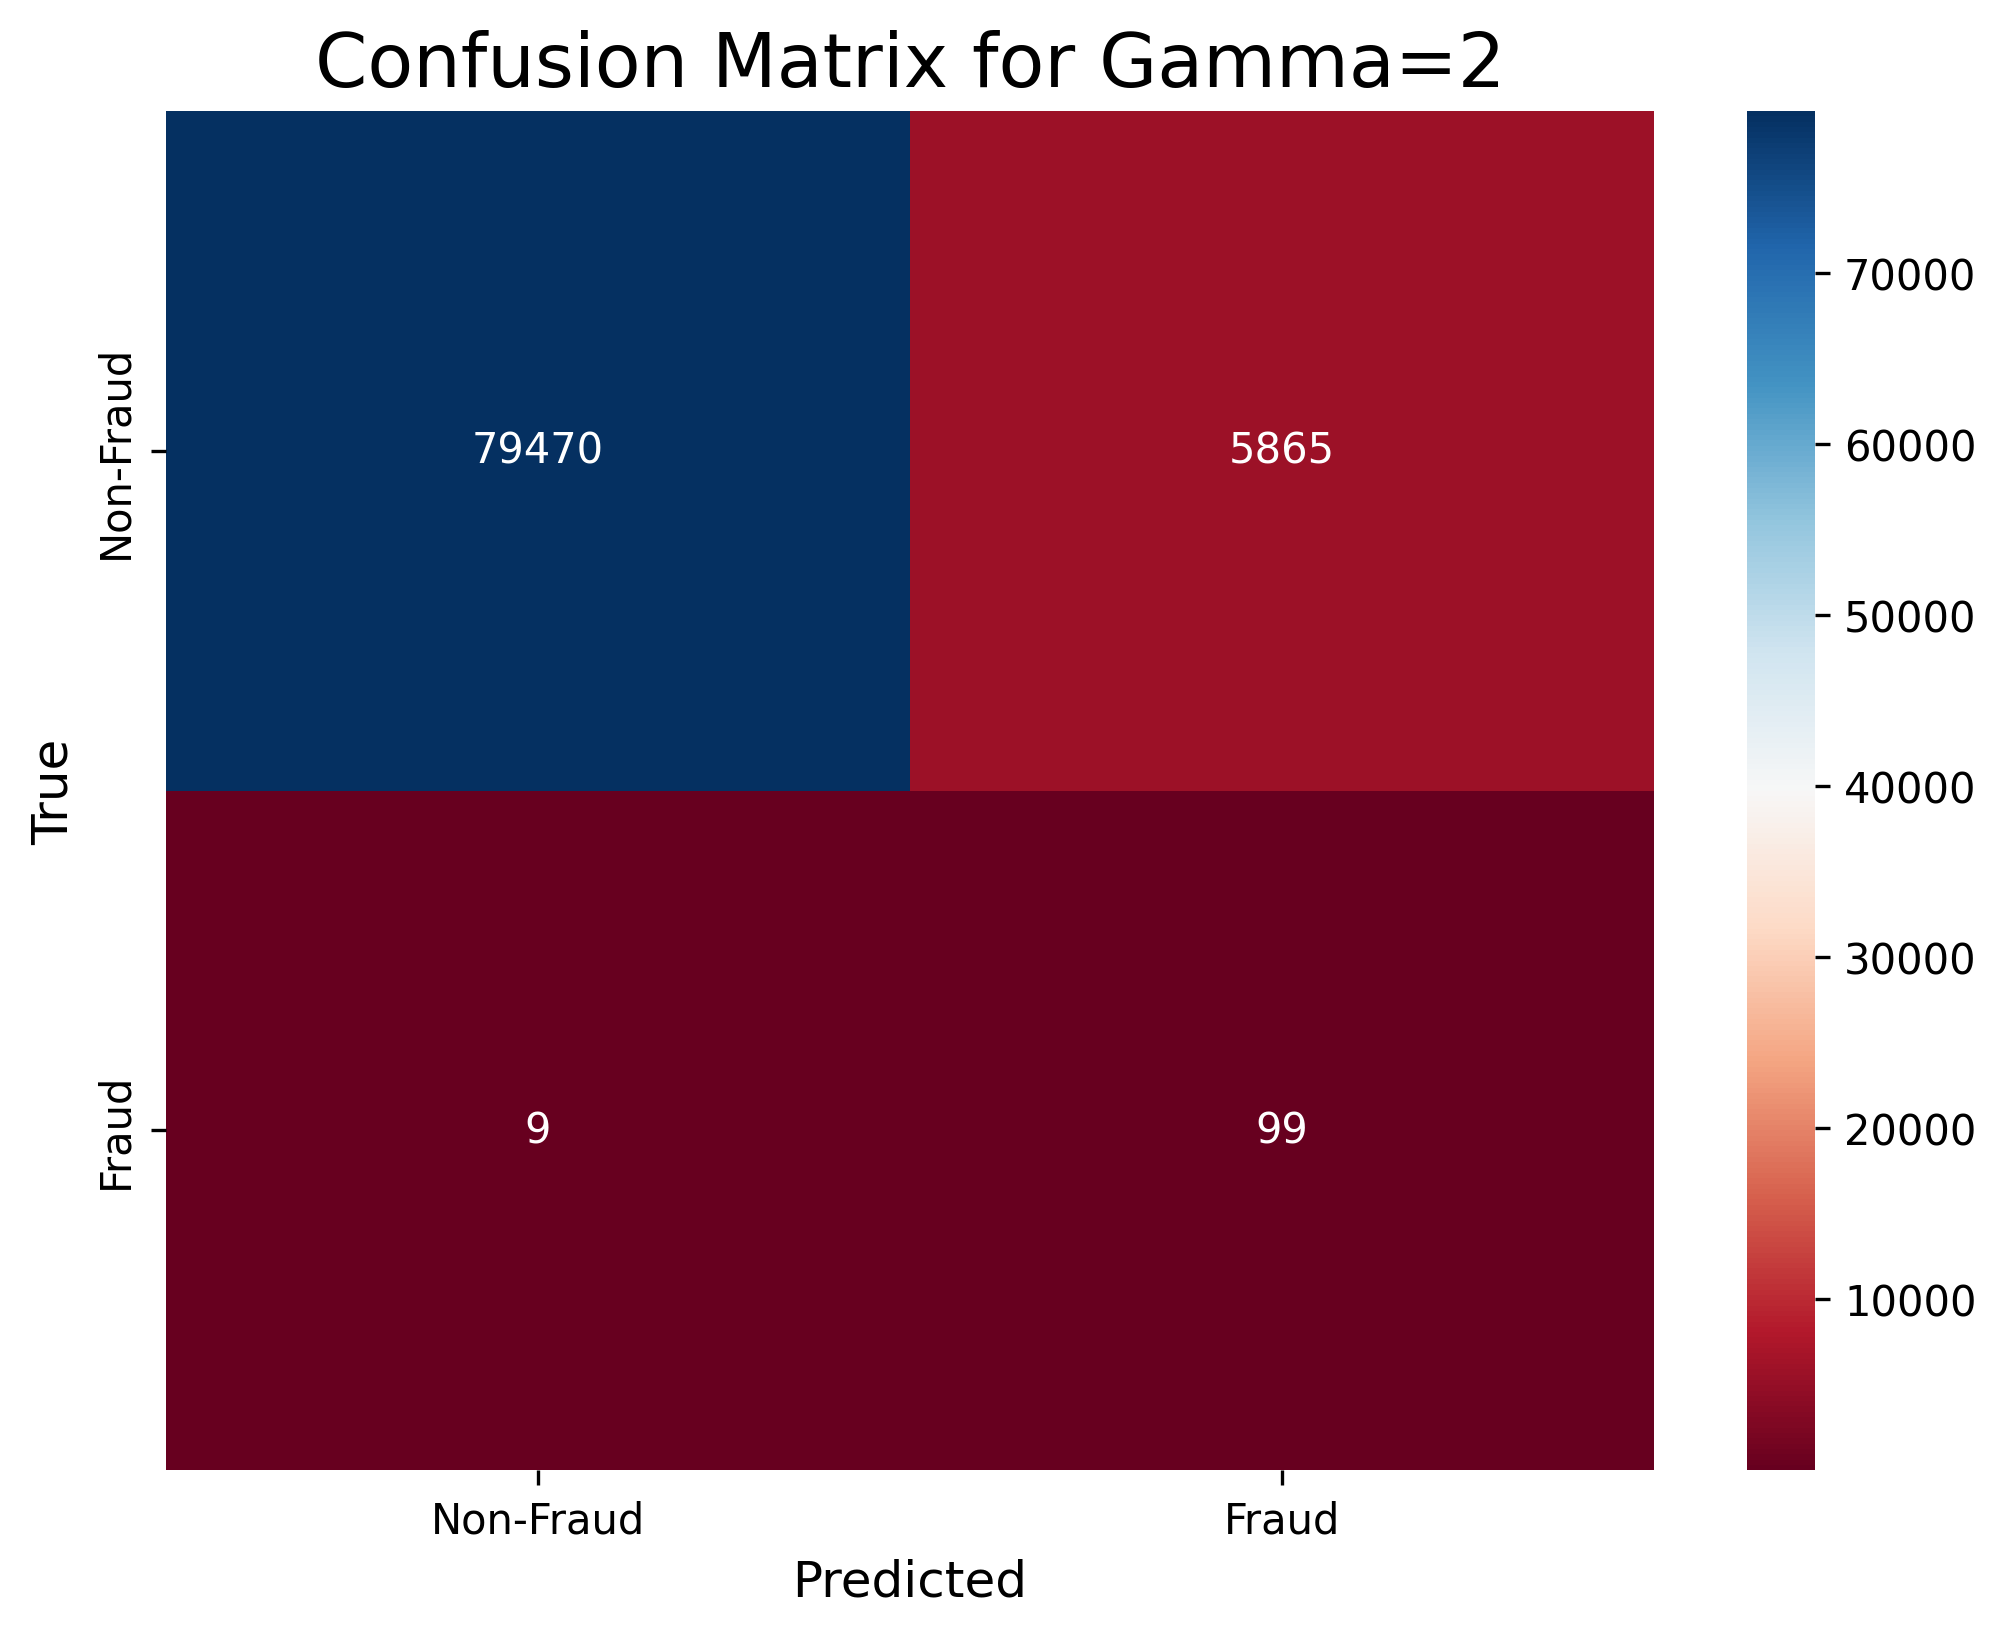
\includegraphics[width=1.0\textwidth]{images/confusion_matrix_transformer_2.png}
        \caption{Confusion Matrix for Transformer With Gamma = 2}
        \label{fig:confusion_matrix_transformer_2}
    \end{minipage}\hfill
    \begin{minipage}{0.49\textwidth}
        \centering
        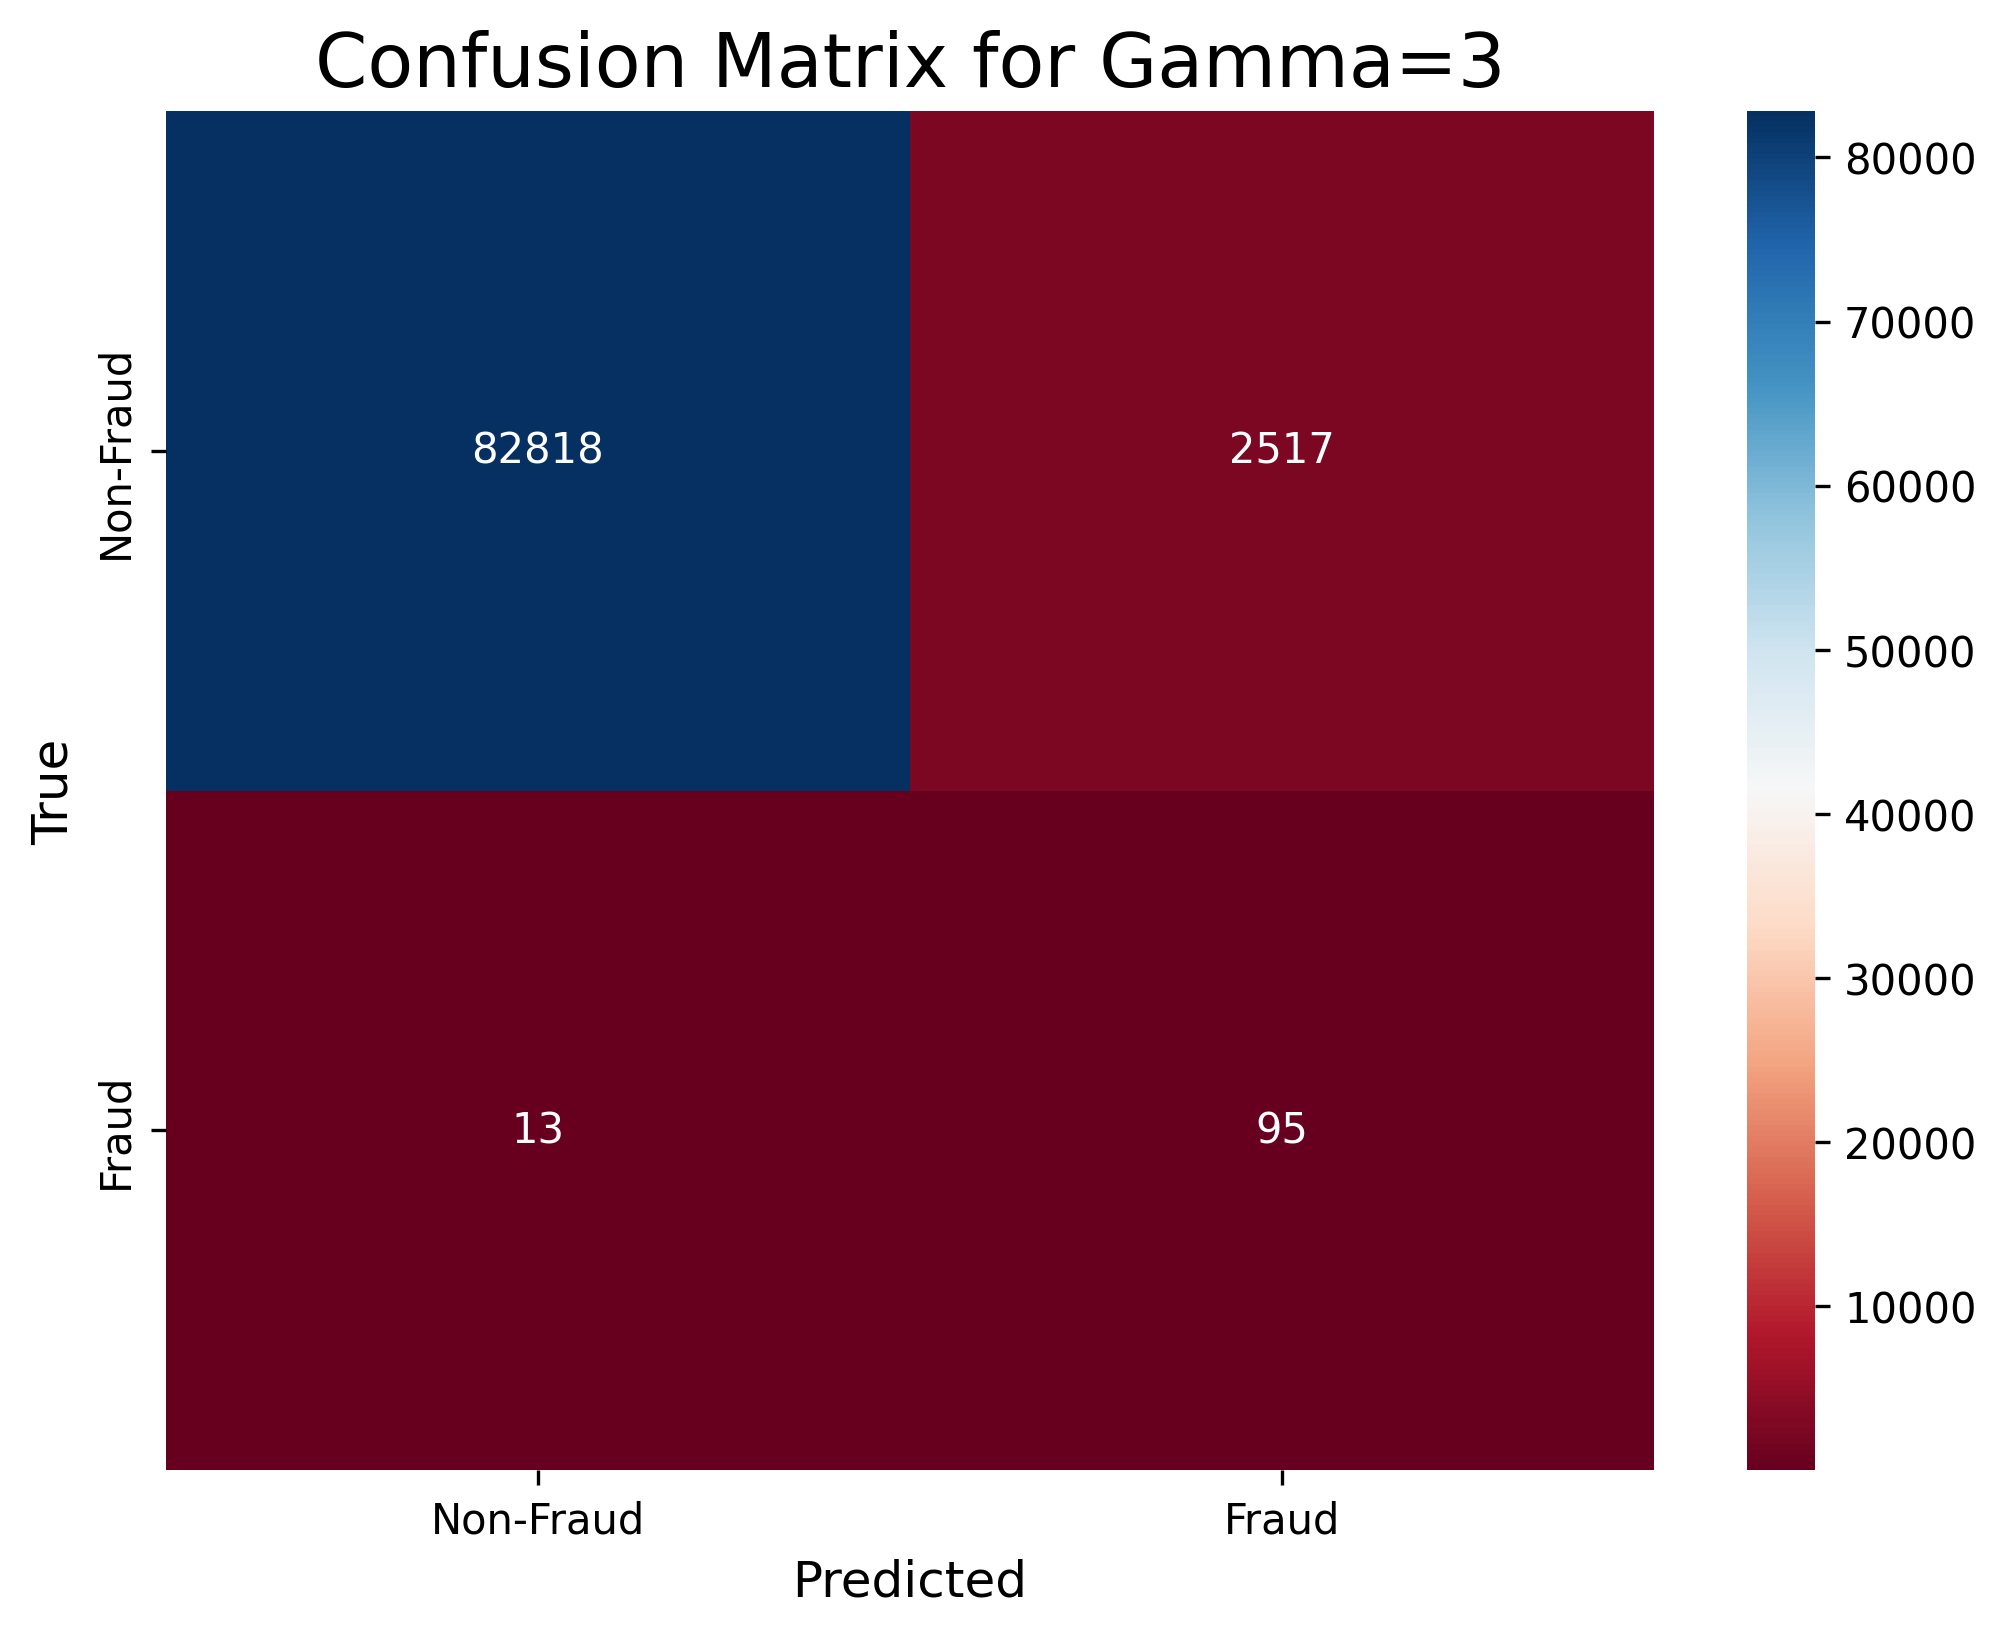
\includegraphics[width=1.0\textwidth]{images/confusion_matrix_transformer_3.png}
        \caption{Confusion Matrix for Transformer With Gamma = 3}
        \label{fig:confusion_matrix_transformer_3}
    \end{minipage}
\end{figure}

\begin{figure}[H]
    \centering
    \begin{minipage}{0.49\textwidth}
        \centering
        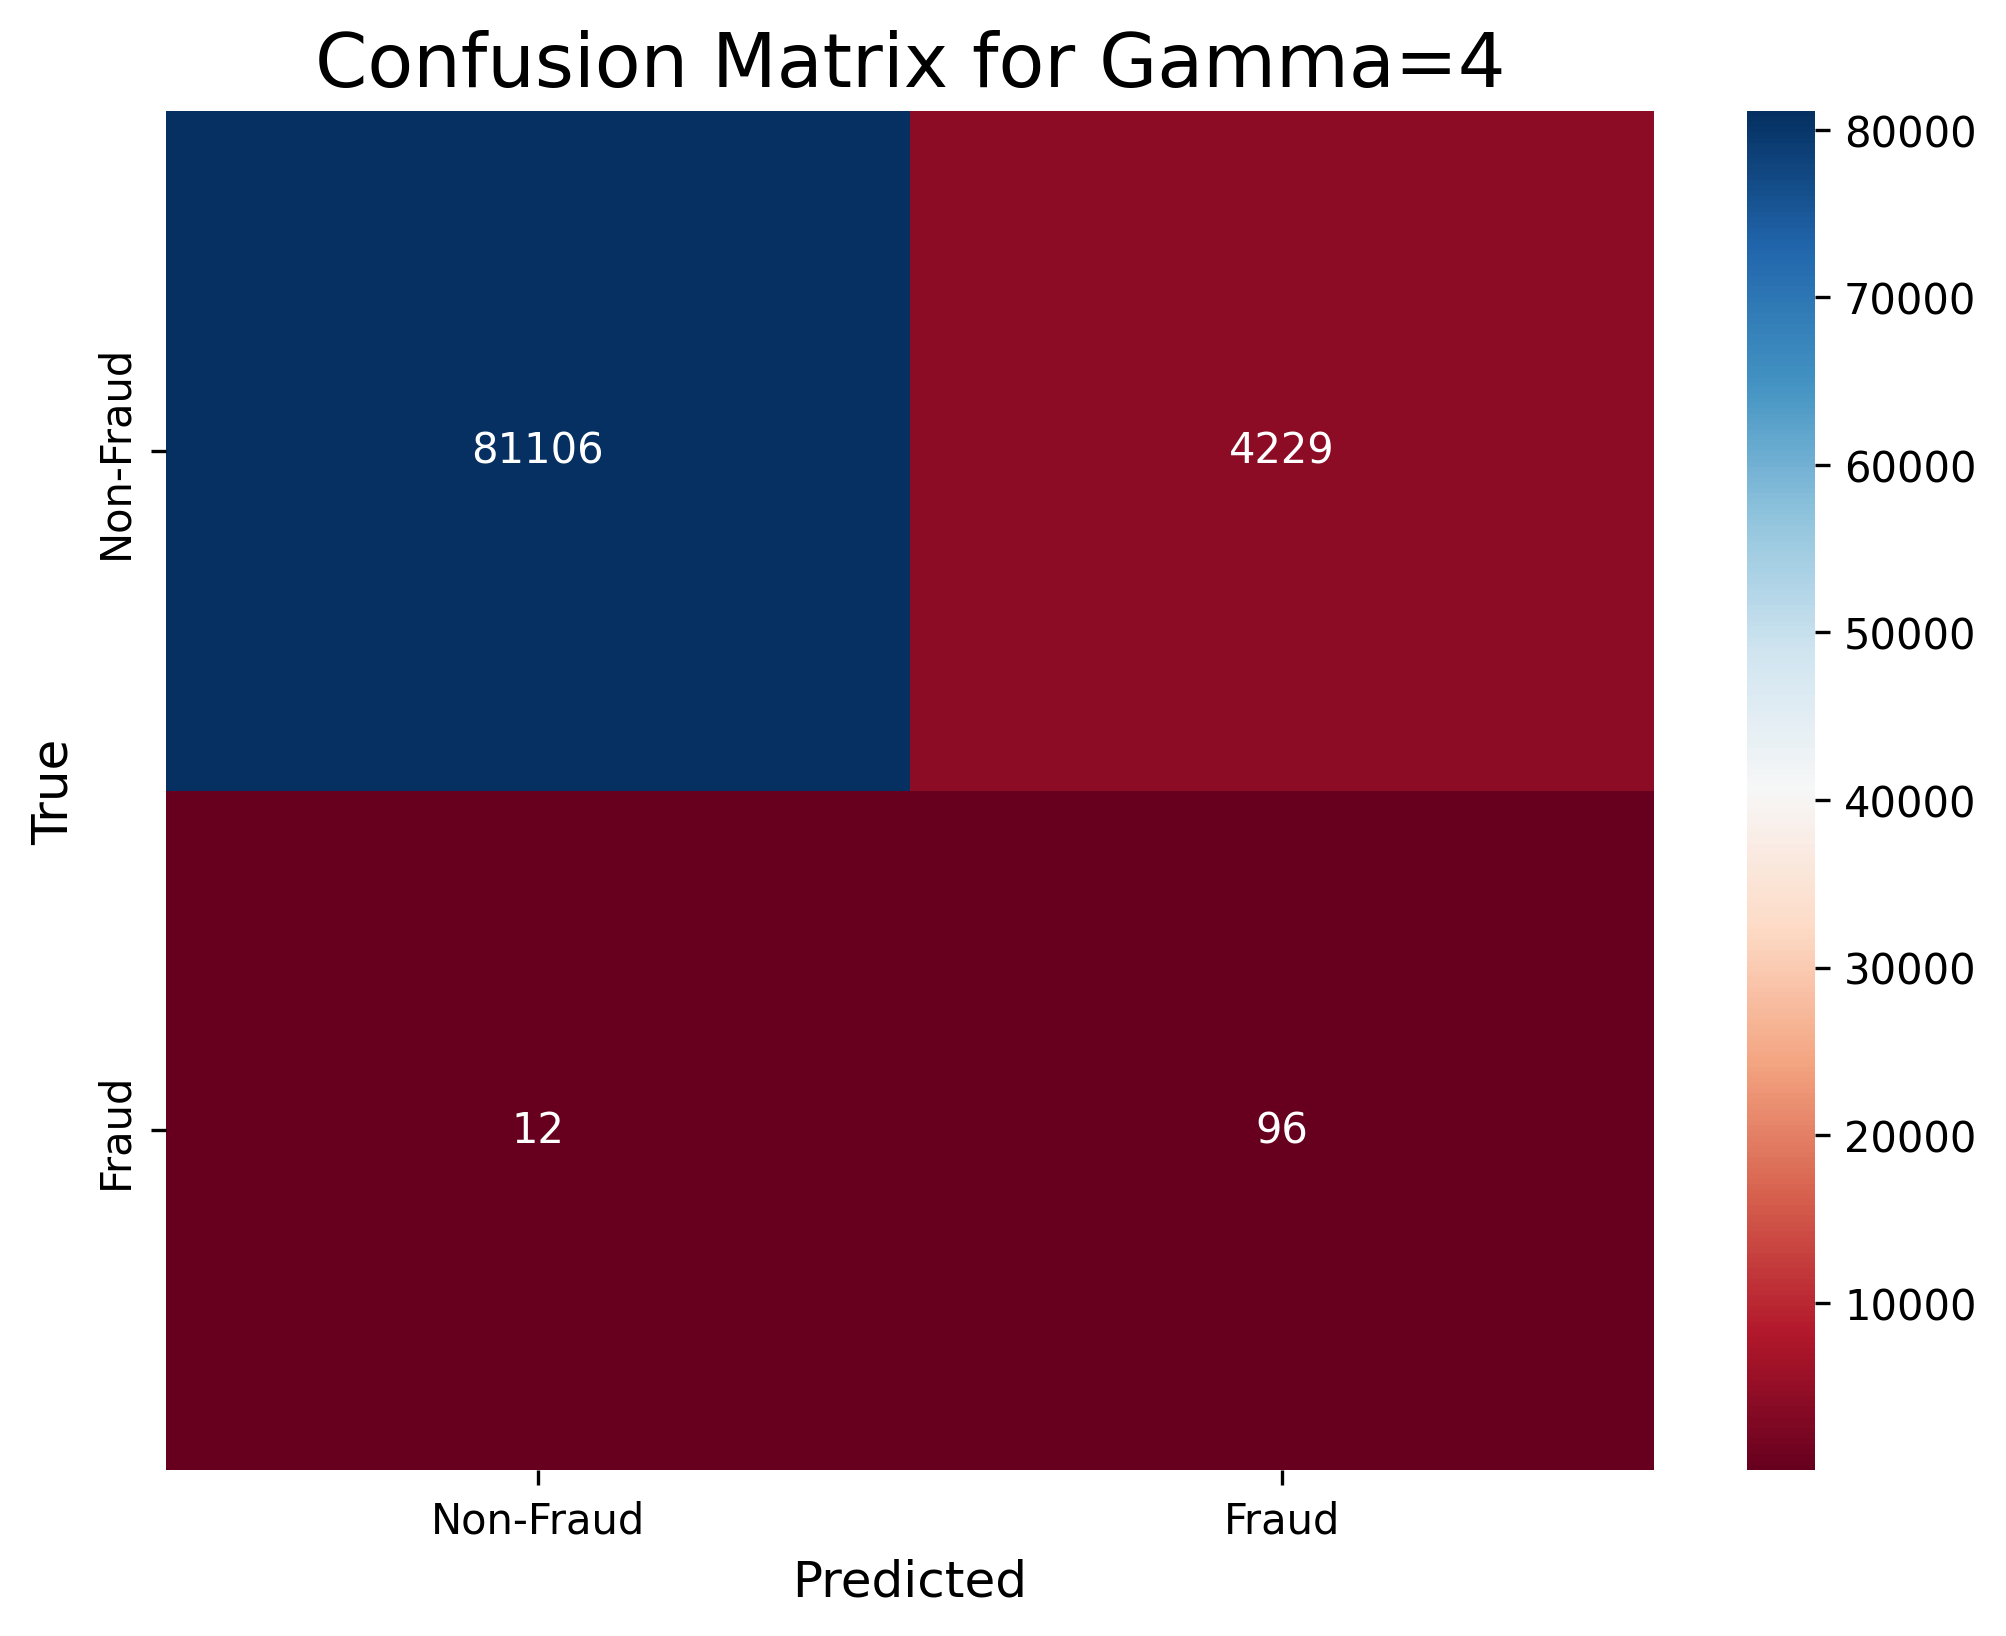
\includegraphics[width=1.0\textwidth]{images/confusion_matrix_transformer_4.png}
        \caption{Confusion Matrix for Transformer With Gamma = 4}
        \label{fig:confusion_matrix_transformer_4}
    \end{minipage}\hfill
    \begin{minipage}{0.49\textwidth}
        \centering
        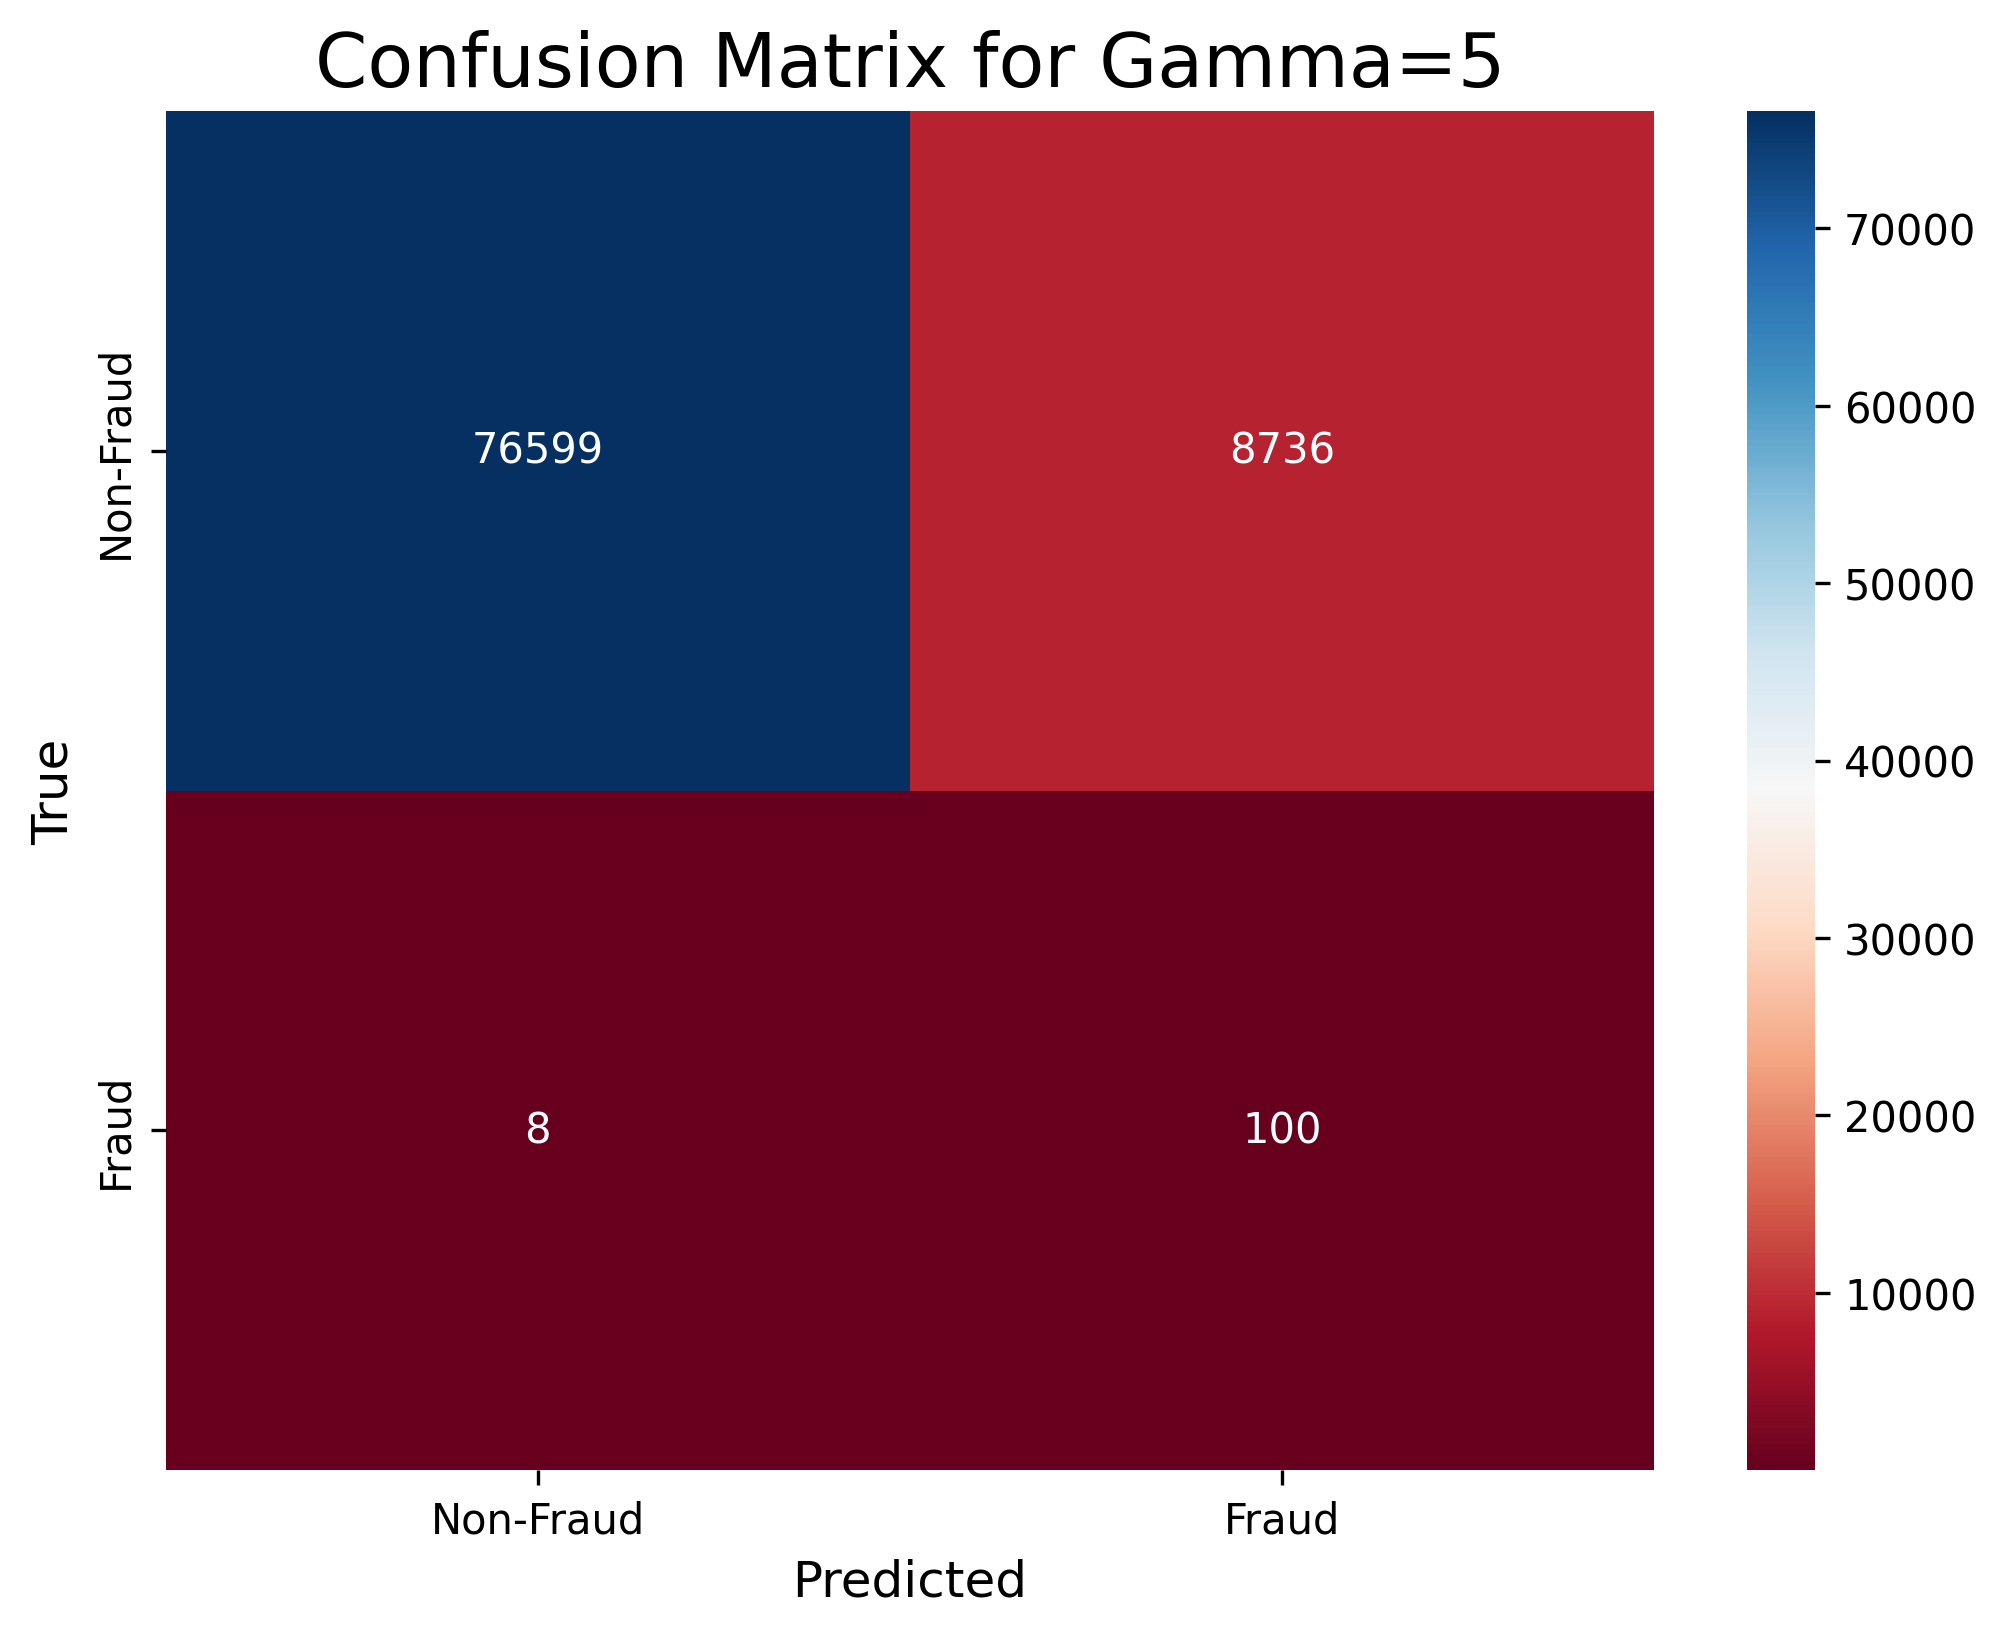
\includegraphics[width=1.0\textwidth]{images/confusion_matrix_transformer_5.png}
        \caption{Confusion Matrix for Transformer With Gamma = 5}
        \label{fig:confusion_matrix_transformer_5}
    \end{minipage}
\end{figure}

To gauge the significance of these results, we also trained an LSTM model using Focal Loss with \(\gamma = 2\). Despite the LSTM’s capacity for modeling sequential patterns, it did not match the Transformer's performance. Specifically, the LSTM achieved a fraud recall of 0.75 and an ROC AUC of approximately 0.875 under the same conditions, as indicated by its confusion matrix and classification report. This contrast suggests that the Transformer's attention mechanism and its flexible capacity to reweight features may better capitalize on the adjustments introduced by Focal Loss.

\begin{figure}[H]
    \centering
    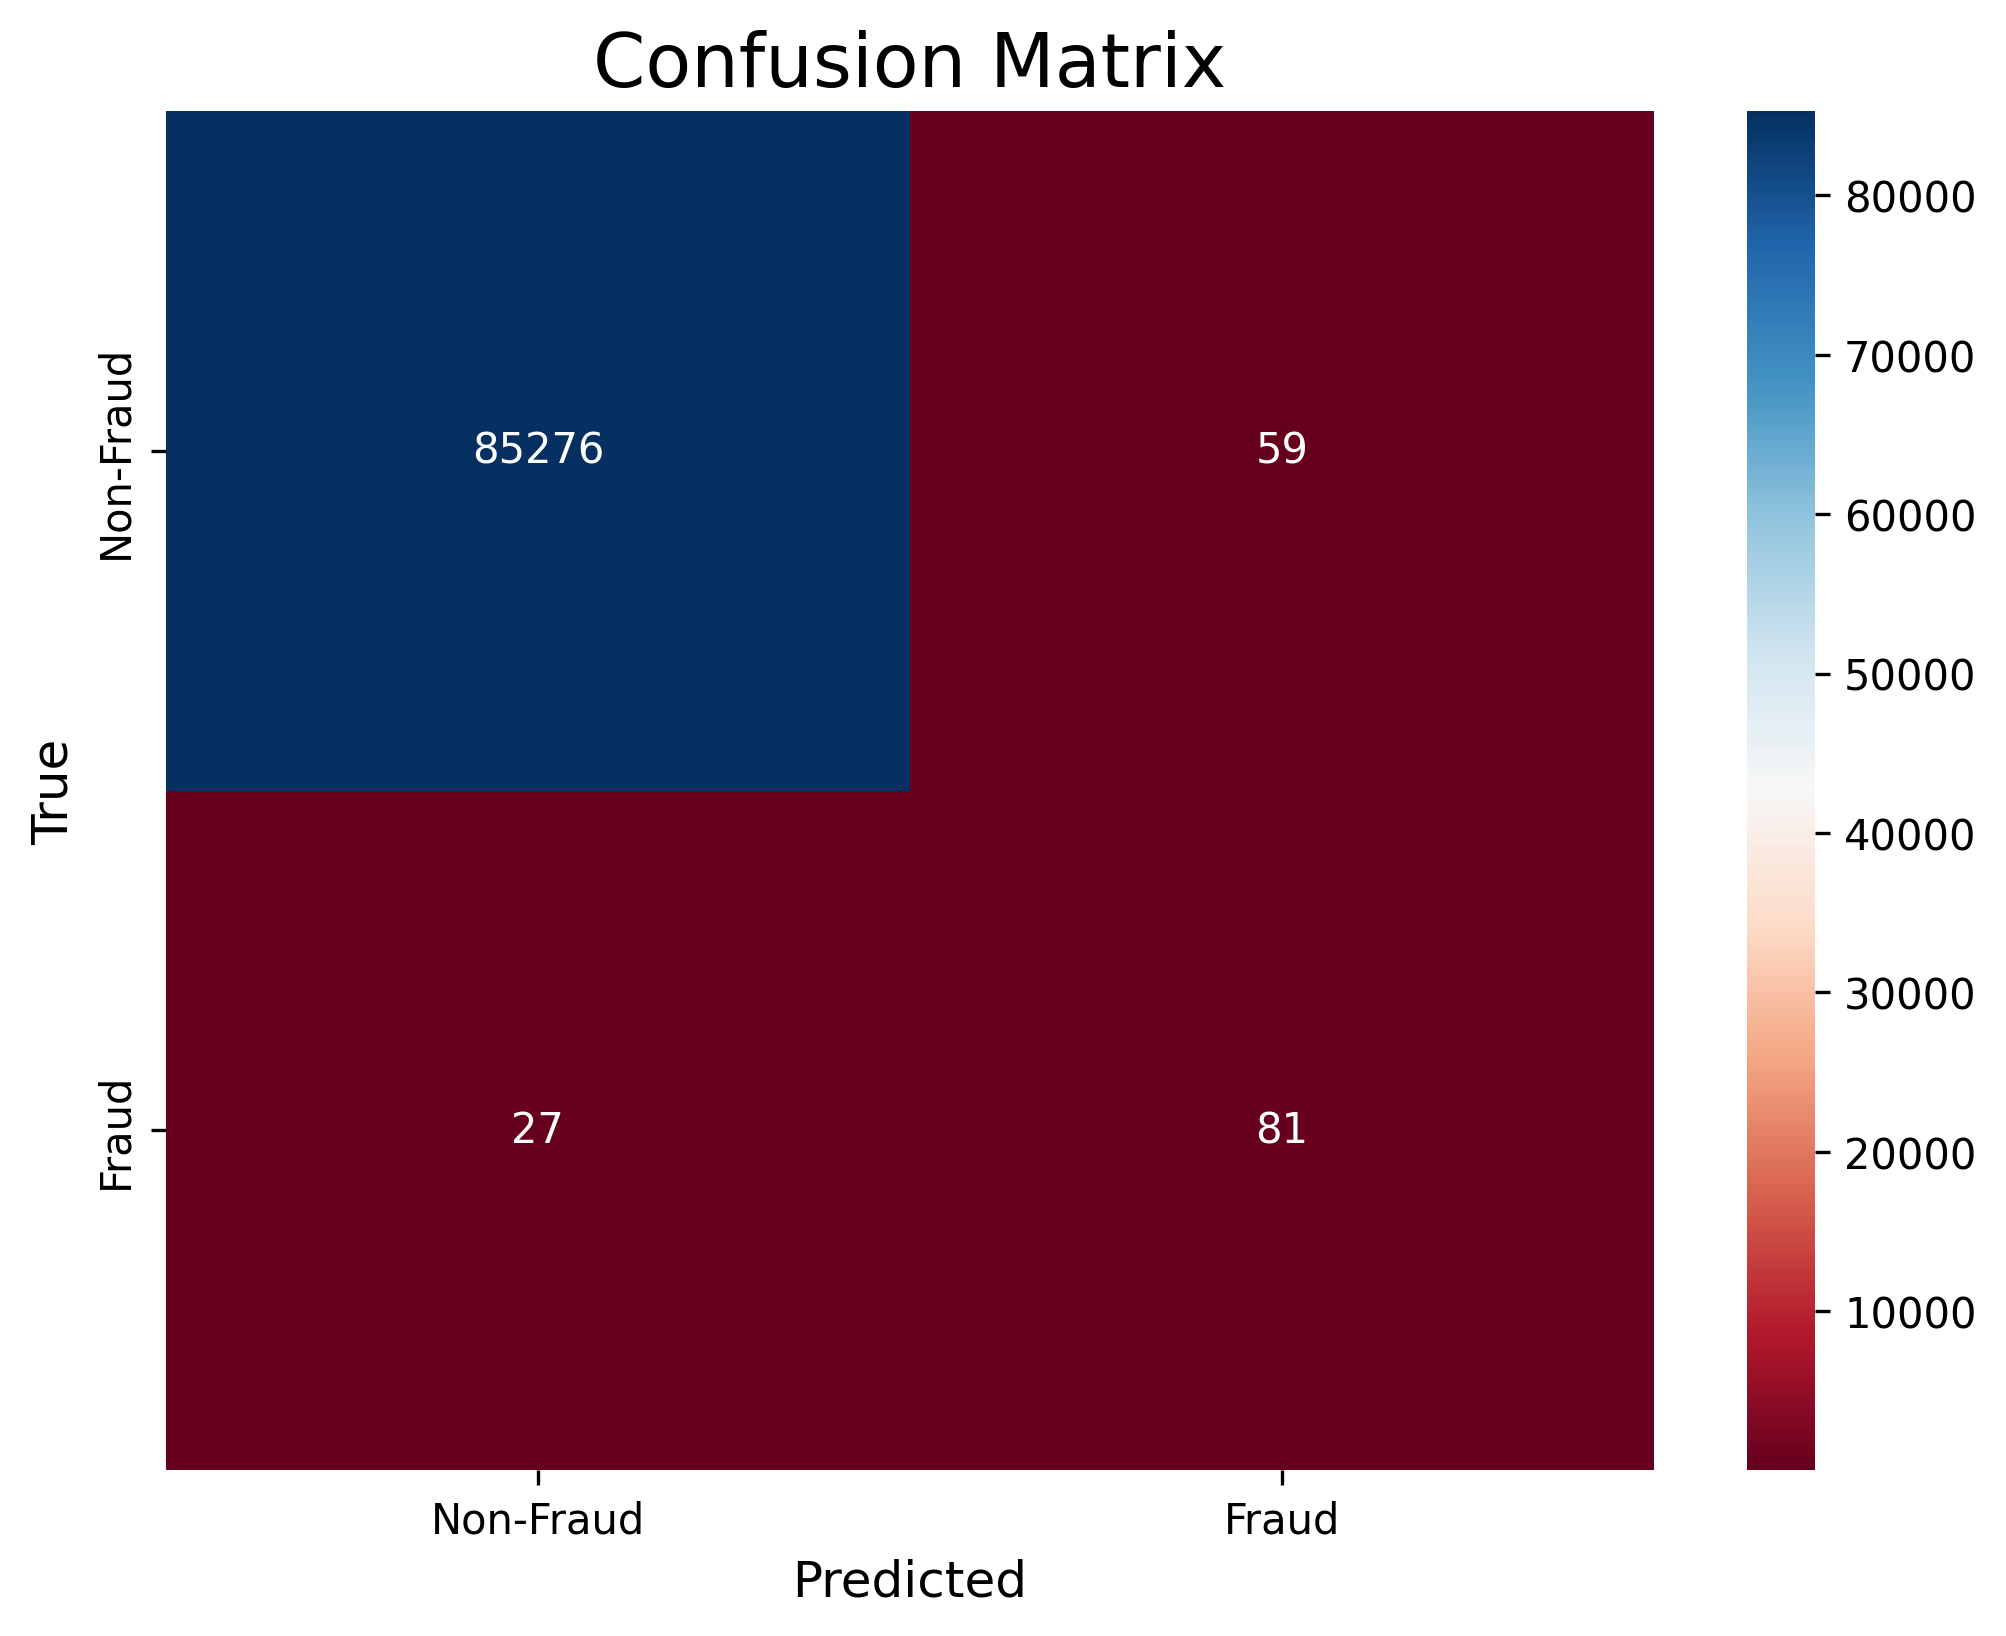
\includegraphics[width=0.65\textwidth]{images/confusion_matrix_lstm_2.png}
    \caption{Confusion Matrix for LSTM With Gamma = 2}
    \label{fig:confusion_matrix_lstm_2}
\end{figure}

\subsection{Comparison with Logistic Regression}

It is noteworthy that, prior to fine-tuning the Transformer with Focal Loss, Logistic Regression performed surprisingly well after SMOTE balancing. Achieving a fraud recall of 0.90, Logistic Regression set a high baseline for more complex models. Only when carefully tuning parameters—such as applying Focal Loss with \(\gamma = 2\)—was the Transformer able to surpass Logistic Regression’s minority-class recall.

Several factors can contribute to this outcome:

1. \textbf{Data Linearity:} The PCA-transformed features may not require a complex decision boundary. If the minority class becomes more separable after SMOTE, a linear model like Logistic Regression can perform exceedingly well.

2. \textbf{Regularization and Tuning:} More complex models, such as the Transformer, are prone to overfitting if not carefully tuned. Identifying the right \(\gamma\) value for Focal Loss is an example of how parameter adjustments can elevate the Transformer's performance beyond simpler methods.

3. \textbf{Model Complexity vs. Practical Gains:} While complex architectures offer more representational power, they do not guarantee superiority. Empirical evidence—like the results we see here—should guide model selection. The Transformer needed a deliberate combination of class rebalancing (SMOTE) and Focal Loss tuning (\(\gamma = 2\)) to surpass the initial successes of Logistic Regression in identifying fraud.

In summary, the Transformer’s performance, aided by carefully chosen Focal Loss parameters, underscores the importance of targeted fine-tuning. By experimenting with different \(\gamma\) values, we identified a configuration that outperforms Logistic Regression on the minority class, demonstrating that sophisticated architectures can indeed surpass simpler models when optimally calibrated. However, these results also emphasize that complex solutions may require more experimentation and tuning to realize their full potential in fraud detection tasks.


\section{Conclusion and Future Work}

This study demonstrates that a Transformer-based model, combined with SMOTE and an appropriately tuned Focal Loss, can enhance fraud detection in severely imbalanced credit card transaction data. Our experiments reveal that while Logistic Regression, once balanced with SMOTE, sets a surprisingly high standard for minority-class recall, the Transformer can ultimately surpass it by carefully adjusting the focusing parameter \(\gamma\). The results confirm that more complex architectures do not inherently guarantee better performance; rather, thoughtful model selection, data preprocessing, and hyperparameter tuning are critical to achieving superior results.

The absence of a separate validation set in this project was a deliberate choice, made to maximize the utilization of the limited minority-class examples. Nevertheless, this approach may risk overfitting and limit our ability to robustly assess model generalization. In future work, we intend to explore time series cross-validation techniques to better evaluate model performance and enhance generalization under realistic temporal conditions. Additionally, while we focused on model performance, future research could consider incorporating interpretability methods to provide actionable insights for fraud analysts. Experimenting with more sophisticated architectures or integrating external data sources may also further improve fraud detection rates.

By continuing to refine these techniques, we aim to develop more reliable and generalizable fraud detection solutions that can adapt to evolving patterns and constraints in financial transaction data.

\newpage
\bibliographystyle{unsrt}
\bibliography{references}



\end{document}